%---------------------------------------------------------------------------%
%-                                                                         -%
%-                           LaTeX Template                                -%
%-                                                                         -%
%---------------------------------------------------------------------------%
%- Copyright (C) Huangrui Mo <huangrui.mo@gmail.com>
%- This is free software: you can redistribute it and/or modify it
%- under the terms of the GNU General Public License as published by
%- the Free Software Foundation, either version 3 of the License, or
%- (at your option) any later version.
%---------------------------------------------------------------------------%
%->> Document class declaration
%---------------------------------------------------------------------------%
\documentclass[doublesided]{Style/ucasthesis}%
%- Multiple optional arguments:
%- [<singlesided|doublesided|printcopy>]% set one or two sided eprint or print
%- [fontset=<adobe|...>]% specify font set to replace automatic detection
%- [plain]% thesis writing of international students
%- [draftversion]% show draft version information
%- [standard options for ctex book class: draft|paper size|font size|...]%
%---------------------------------------------------------------------------%
%->> Document settings
%---------------------------------------------------------------------------%
\usepackage[authoryear,myhdr,list]{Style/artratex}% document settings
%- usage: \usepackage[option1,option2,...,optionN]{artratex}
%- Multiple optional arguments:
%- [bibtex|biber]% set bibliography processor and package
%- [<numbers|super|authoryear|alpha>]% set citation and reference style
%- <numbers>: textual: Jones [1]; parenthetical: [1]
%- <super>: textual: Jones superscript [1]; parenthetical: superscript [1]
%- <authoryear>: textual: Jones (1995); parenthetical: (Jones, 1995)
%- <alpha>: textual: not available; parenthetical: [Jon95]
%- [geometry]% reconfigure page layout via geometry package
%- [lscape]% provide landscape layout environment
%- [myhdr]% enable header and footer via fancyhdr package
%- [color]% provide color support via xcolor package
%- [background]% enable page background
%- [tikz]% provide complex diagrams via tikz package
%- [table]% provide complex tables via ctable package
%- [list]% provide enhanced list environments for algorithm and coding
%- [math]% enable some extra math packages
\usepackage{Style/artracom}% user defined commands
%---------------------------------------------------------------------------%
\newcommand \hi  {H{\small I}\ }
\newcommand \hii {H{\small II}\ }
\newcommand \nh  {N$_{\rm H}$\ }
\newcommand \co  {$^{13}$CO \ }
\newcommand \kms {km s$^{-1} \ $}
\newcommand \as  {$^{\prime\prime}~$}
\newcommand \am  {$^{\prime}~$}
\newcommand{\aap}{A\&A}
\newcommand{\aaps}{A\&AS}
\newcommand{\mnras}{MARAS}
\newcommand{\apj}{ApJ}
\newcommand{\apjl}{ApJL} % need to check
\newcommand{\apjs}{ApJS}
\newcommand{\pasj}{PASJ}
\newcommand{\aj}{AJ}
\newcommand \raa  {RAA}
\newcommand \jkas {JKAS}
%---------------------------------------------------------------------------%
%\includeonly{Tex/Chap_1,...,Tex/Chap_N}% selected files compilation
%---------------------------------------------------------------------------%
%->> Document content
%---------------------------------------------------------------------------%
\begin{document}
%-
%-> Frontmatter: title page, abstract, content list, symbol list, preface
%-
\frontmatter% initialize the environment
%---------------------------------------------------------------------------%
%->> 封面信息及生成
%---------------------------------------------------------------------------%
%-
%-> 中文封面信息
%-
\confidential{}% 密级:只有涉密论文才填写
\schoollogo{scale=0.095}{ucas_logo}% 校徽
\title{复杂星周环境中超新星遗迹的磁流体模拟}% 论文中文题目
\author{张孟飞}% 论文作者
\advisor{田文武~研究员~张海燕~研究员}% 指导教师:姓名 专业技术职务 工作单位
\advisors{中国科学院国家天文台}
\degree{博士}% 学位:学士、硕士、博士
\degreetype{理学}% 学位类别:理学、工学、工程、医学等
\major{天体物理}% 二级学科专业名称
\institute{中国科学院国家天文台}% 院系名称
\date{2019~年~6~月}% 毕业日期:夏季为6月、冬季为12月
%-
%-> 英文封面信息
%-
\TITLE{Magnetohydrodynamics Simulation for Supernova\\Remnants in
Complex Circumstellar Environment}% 论文英文题目
\AUTHOR{Zhang Mengfei}% 论文作者
\ADVISOR{Supervisor: Profs. TIAN Wenwu \& ZHANG Haiyan}% 指导教师
\DEGREE{Doctor}% 学位:Bachelor, Master, Doctor。封面格式将根据英文学位名称自动切换,请确保拼写准确无误
\DEGREETYPE{Philosophy}% 学位类别:Philosophy, Natural Science, Engineering, Economics, Agriculture 等
\THESISTYPE{Dissertation}% 论文类型:thesis, dissertation
\MAJOR{Astrophysics}% 二级学科专业名称
\INSTITUTE{National Astronomical Observatories of China\\Chinese Academy of Sciences}% 院系名称
\DATE{June, 2019}% 毕业日期:夏季为June、冬季为December
%-
%-> 生成封面
%-
\maketitle% 生成中文封面
\MAKETITLE% 生成英文封面
%-
%-> 作者声明
%-
\makedeclaration% 生成声明页
%-
%-> 中文摘要
%-
\chapter*{摘\quad 要}\chaptermark{摘\quad 要}% 摘要标题
\setcounter{page}{1}% 开始页码
\pagenumbering{Roman}% 页码符号

超新星遗迹(SNR)是超新星爆发后与周围星际介质相互作用的产物,其产生过程涉及天体物理、粒子物理、
分子化学等多个领域,是目前天文研究中的前沿课题之一。通过观测SNR并分析其中元素丰度、动力学特性,我们
可以估算其前身星类型,为超新星爆发模型提供参考;同时基于其多波段能谱(SED),我们可以剖析其中粒子加速
机制,为宇宙线的起源找到更加合理的解释;而对其分子谱线的观测研究,也让我们能进一步理解星际介质和
星系中分子生成与破坏的过程。这些过程都与超新星遗迹的演化密不可分。 最近几十年以来,对SNR演化过程及对
周边物质影响的研究有了更深入的了解,但没解决的难点问题依然很多,尤其对SNR在不同环境里的演化细节和
物理机制知道得还很不充分。对SNR更多新的观测和深入的理论探讨依然是非常必要的。

研究超新星遗迹演化主要的困难在于众多SNR所处物理环境很不一样,单一的解析模型无法解释很多遗迹的观测结果。
因此,我们需要一个基于简洁明了的理论,能梳理清楚复杂情况的方法来研究超新星遗迹的演化,而磁流体
模拟正是最佳选择。磁流体模拟的重点在于对初始条件的选取,可因为初始条件实质上就是过去发生的事,
所以理论上我们永远无法得知一个遗迹的准确初始条件。实际上,有一些爆发时就观测到的
历史超新星遗迹可以得到较为可靠的爆发能量及抛射质量,尤其是SN 1987A,可以说是研究超新星遗迹演化的
范本。但是这些遗迹数量很少,不具有普适性,对于银河系中已经观测到的300多个遗迹,绝大部分前身星
的性质并不清楚。此外,超新星遗迹的演化受到星周介质的巨大影响,而通常星周介质初始的
密度、磁场等性质更难得到。于是,很多对超新星遗迹的模拟都假设均匀、线性或者幂律的星周介质分布,
这与实际复杂的介质分布相差甚远,所以也很难解释有不同表象的观测结果。

本文尝试寻找更好的方法解决这两方面的困难,主要的工作有:
\begin{itemize}
  \item 基于对SNR的X射线观测得到的元素丰度、电子密度估计,结合射电波段对超新星遗迹的HI测距,估算较为可靠前身星
  爆发能量、抛射物质量,结合磁流体模拟,互相验证参数估计。
  我们选择观测研究较多的SNR W51C为例,以方便检验模拟结果。
  前人已经粗略估算出其前身星质量和爆发能量,可是我们经过初步模拟发现,这样的参数无法模拟这颗遗迹,
  同时也违背了最近通过观测得到的超新星爆发质量-能量的经验模型。
  通过检验,我们发现前人估算爆发能量使用的距离并不合理,最终我们建议使用更合理的距离4.3 kpc和爆发能量
  1.3 $\times$ 10$^{51}$ ergs s$^{-1}$。

  \item 为了得到SNR W51C的单边厚壳层,我们采取了普遍使用的设置磁场梯度的方法,偶然发现了SNR W51C
  应该存在一个新的壳层。
  超新星爆发时如果星周介质存在一个磁场梯度,那么最终演化结果可能会是一个单壳层的超新星遗迹。
  而SNR W51C一直被认为是一个单壳层的遗迹,而我们的模拟结果显示其存在一个可能暗弱但仍然能够被观测
  到的壳层。
  通过查看射电图像我们判断,这一新壳层很可能已被观测到,但因为与周围电离氢区在视线方向重合,所以一
  直没有被分离出来,而后来对该SNR射电偏振图像的分析证实了我们的猜测。

  \item SNR W51C同时也是一个少见的TeV伽马射线源,被认为与分子云(MC)相互作用。
  我们模拟了其沿视线方向与分子云相互作用,结果显示这种相互作用可能导致局部磁场放大,射电流量增强,
  从而可能在遗迹的中心区域观测到射电辐射。
  而对临近SNR W51C中心区域的射电偏振、非热辐射及羟基(OH)谱线图的分析,证实了这种相互作用方式的
  存在。

  \item 我们认为一个大质量恒星晚期的星风对其爆发为超新星时的星周介质有很大影响。
  通过模拟星风,并以星风模拟结果作为星周介质的初始条件,我们很好地模拟了超新星遗迹演化,以此为
  基础我们能够解释很多之前无法解释的遗迹形态,比如八字形和大弧度单边遗迹。

  \item 以考虑星风的超新星遗迹模拟为基础,我们认为前身星星风可以大大影响遗迹局部的磁场及介质分布。
  前人曾经通过观测超新星遗迹的磁场来估算银河系大尺度的磁场分布,而我们的这一工作表明,这种估算磁场
  的方式有严格限制条件,不然会出现问题。

  \item 通过模拟SNR在强磁场环境中的演化,我们发现多壳层遗迹的形成、奇特的SNR射电和X射线轮廓、费米泡
  的形成或许都与强磁场有关。
\end{itemize}

本文在模拟中采用更为合理的复杂星周环境,从而更准确地研究SNR演化。
根据结果,我们也得到很多之前没有注意到的演化特征,以及由此而来的推论。
不仅解释了广受关注的SNR W51C中存在多年的问题,也首次通过模拟星风-超新星遗迹系统来解释
SNR的多种射电形态,同时首次研究了强磁场极端条件下的SNR演化。
这些工作对我们进一步理解SNR演化过程具有极大参考价值。

\keywords{星际介质:超新星遗迹 - 磁流体模拟 - 星际介质:SNR W51C - 方法:数值模拟}% 中文关键词
%-
%-> 英文摘要
%-
\chapter*{Abstract}\chaptermark{Abstract}% 摘要标题

Supernova remnant (SNR) results from the interaction between shock wave of supernova
and circumstellar medium (CSM), a process related to astrophysics, particle physics and molecule
chemistry, etc.
To study SNRs and its interaction with the CGM is a frontier project in astronomical
researches.
By observing an SNR and analyzing its abundance and the kinematics, we can derive
the type of its progenitor, which will provide indication for models of supernova explosion.
Meanwhile, based on its spectral energy distribution (SED) at multiband, we can disentangle
the intrinsic acceleration mechanism, and understand the origin of cosmic rays better.
In addition, the spectral observation to an SNR can help us understand the formation
and destruction of molecule in ISM of a galaxy.
To study SNRs may help to figure out these issues, the detail how an SNR is involving has
not been well understood.

The real picture of the SNR's evolution is complex in evolution of SNR, so it is difficult to study
the details by using a traditional analytical model.
Therefore, we need a model-based method to get the situation sorted.
The magnetohydrodynamics (MHD) simulation is the best choice for our case.
The key point of the MHD simulation is to choose initial conditions.
Initial conditions are actually the past things, so we theoretically will never know
the accurate initial conditions of the evolution of an SNR without perfect history record.
The reliable initial conditions of some historical SNRs may be estimated if they have well
been monitored before its explosion.
For example, SN 1987A is known as a gift of God.
Nevertheless, there are only several historical SNRs so that we are not able to use them to explain
most of about 300 SNRs already detected in Milky Way.
Moreover, the evolution of SNRs is strongly influenced by CSM, which leads
 more difficult to estimate the initial density and magnetic field of CSM.
Many simulations for SNRs are assumed to have homogeneous, liner, power-law or
exponential density distribution, which is completely different from the reality, so we fail in
using these simulation to  explain many observational phenomena.

In this paper, we describe the better method to solve the issues mentioned above. The primary
results are shown as follows:
\begin{itemize}
   \item By using the estimation of abundance and electron density based on X-ray observations
   of an SNR and the distance of an SNR by the HI observation, we can estimate the explosion
   energy and ejecta mass of its progenitor.
   We may further check the parameters by comparing observations and simulations.
   We choose the well-studied SNR W51C as an example, so that we can test whether we perform the
   simulation correctly.
   Previous researchers have estimated its progenitor mass and explosion energy, but we cannot
   successfully simulate this SNR by applying such parameters.
   We find these parameters are also inconsistent with that from the derived mass-energy model
   based on recent observation.
   We therefore analyze the methods and parameters carefully and finally take a recently-measurement
   distance of 4.3 kpc and an explosion energy of 1.3 $\times$ 10$^{51}$ ergs s$^{-1}$ as the
   initial parameter of W51C.

   \item To simulate the thick unilateral shell, we set a gradient of magnetic field, a method
   often used to obtain such shell.
   By analyzing the results, we find there should be a new shell of SNR W51C.
   A supernova will evolve to an SNR with unilateral shell, if there exists a magnetic field
   gradient.
   SNR W51C presents a clear semi-shell in previous study, but our simulation shows there is
   possibly another new edge which is much darker but should be detected by previous observations
   with enough sensitivity.
   We investigate its radio images and conclude this new edge overlaps with a radio-strong HII
   region.
   Further analysis aiming at radio polarization map also confirms our result.

   \item SNR W51C is also a TeV $\gamma$-ray source, suggested previously to interact with molecular
   clouds (MCs).
   We simulate how it interacts with an MC along the line of sight (LoS). We find that this process
   can amplify the magnetic field and enhance local radio flux.
   As a result, we can detect radio radiation next to the center of this SNR.
   Meanwhile, we study the radio polarization, non-thermal radiation and OH spectral map in this
   region, which supports such an interaction.

   \item We think the stellar wind of a massive progenitor will largely change the circumstellar
   magnetic field and density distribution.
   We simulate the stellar wind, and take the result as initial conditions for SNR simulation,
   which can help us obtain more accurate simulation.
   This simulation shows a clue to explain many unsolved radio morphologies of SNRs, such as
   bilateral asymmetric and unilateral large-radian SNRs.

   \item Based on the simulation of stellar wind, we notice the stellar wind of progenitor will
   strongly influence local magnetic field.
   However, some researchers try to estimate large-scale magnetic field distribution by
   observing the magnetic field of SNRs, which will need be carefully treated if our simulation
   is correct.

   \item By simulating the evolution of SNRs in strong magnetic field, we notice
   the formation of multi-layers SNRs, the strange radio and X-ray patterns of SNRs
   and the formation of Fermi bubbles are all possibly related to strong magnetic field.
\end{itemize}

    In this paper, we apply reliable complex circumstellar environment in the simulations,
    so that we can study the evolution of SNRs accurately.
    Based on these simulations, we find many ignored features during the evolution and
    deduce some interesting conclusions.
    We solve some problems related to a well-known SNR W51C, and firstly explain radio
    morphologies of various SNRs by simulating a system simultaneously including stellar wind
    and supernova remnants.
    In addition, we study SNRs evolving in strong magnetic field for the first time.
    These works are very important for understanding the evolution of SNRs.

\KEYWORDS{ISM: supernova remnants – magnetohydrodynamics (MHD) -
ISM: individual objects (W51 C) - method: simulations}% 英文关键词
%---------------------------------------------------------------------------%
% title page, abstract, dedication
{% content list region
\linespread{1.2}% local line space
%\intotoc{\contentsname}% add link to contents table and bookmark
\tableofcontents% contents catalog
%\intotoc{\listfigurename}% add link to contents table and bookmark
\listoffigures% figures catalog
%\intotoc{\listtablename}% add link to contents table and bookmark
\listoftables% tables catalog
}
\chapter*{符号列表}
\chaptermark{符号列表}

\section*{字符}
\nomenclatureitem[\textbf{Unit}]{\textbf{Symbol}}{\textbf{Description}}
\nomenclatureitem[$\Unit{m^{2} \cdot s^{-2} \cdot K^{-1}}$]{$R$}{the gas constant}
\nomenclatureitem[$\Unit{m^{2} \cdot s^{-2} \cdot K^{-1}}$]{$C_v$}{specific heat capacity at constant volume}
\nomenclatureitem[$\Unit{m^{2} \cdot s^{-2} \cdot K^{-1}}$]{$C_p$}{specific heat capacity at constant pressure}
\nomenclatureitem[$\Unit{m^{2} \cdot s^{-2}}$]{$E$}{specific total energy}
\nomenclatureitem[$\Unit{m^{2} \cdot s^{-2}}$]{$e$}{specific internal energy}
\nomenclatureitem[$\Unit{m^{2} \cdot s^{-2}}$]{$h_T$}{specific total enthalpy}
\nomenclatureitem[$\Unit{m^{2} \cdot s^{-2}}$]{$h$}{specific enthalpy}
\nomenclatureitem[$\Unit{kg \cdot m \cdot s^{-3} \cdot K^{-1}}$]{$k$}{thermal conductivity}
\nomenclatureitem[$\Unit{kg \cdot m^{-1} \cdot s^{-2}}$]{$S_{ij}$}{deviatoric stress tensor}
\nomenclatureitem[$\Unit{kg \cdot m^{-1} \cdot s^{-2}}$]{$\tau_{ij}$}{viscous stress tensor}
\nomenclatureitem[$\Unit{1}$]{$\delta_{ij}$}{Kronecker tensor}
\nomenclatureitem[$\Unit{1}$]{$I_{ij}$}{identity tensor}


\section*{缩写}
\nomenclatureitem{AMR}{Adaptive Mesh Refinement}
\nomenclatureitem{BH}{Black Hole}
\nomenclatureitem{CMB}{Cosmic Microwave Background}
\nomenclatureitem{CSM}{Circumstellar Medium}
\nomenclatureitem{DSA}{Diffusive Shock Acceleration}
\nomenclatureitem{ICRF}{International Celestial Reference Frame}
\nomenclatureitem{ISM}{Interstellar Medium}
\nomenclatureitem{MC}{Molecular Cloud}
\nomenclatureitem{MHD}{Magnetohydrodynamics}
\nomenclatureitem{PWN}{Pulsar Wind Nebula}
\nomenclatureitem{RTI}{Rayleigh-Taylor instability}
\nomenclatureitem{RMI}{Richtmyer–Meshkov instability}
\nomenclatureitem{KHI}{Kelvin–Helmholtz instability }
\nomenclatureitem{SED}{Spectral Energy Distribution}
\nomenclatureitem{SNR}{Supernova Remnant}
% list of symbols, preface content
%-
%-> Mainmatter
%-
\mainmatter% initialize the environment
%---------------------------------------------------------------------------%
%->> Main content
%---------------------------------------------------------------------------%
\chapter{引言}
\label{Intro}

\section{超新星遗迹简介}
\label{SNRintro}
超新星遗迹(Supernova Remnants, SNR)是超新星爆发后,其抛射物与周围介质相互作用的产物。
广义的超新星遗迹还包括中心可能残留的致密天体,不过在本文中不予考虑。
第一个有记录可循的观测到的超新星遗迹是蟹状星云(Crab Nebula),这个遗迹是1054年一次超新星
爆发的残骸,虽然超新星爆发本身在当时就被多国天文学家观测到,但是遗迹是过了近700年,才被
约翰·贝维斯和查尔斯·梅西耶分别独立发现\citep{barrow2011cosmic}。
第二个被发现的是开普勒超新星遗迹(Kepler's Supernova Remnant)\citep{Baade1943},这两个
遗迹是射电观测开始之前,唯二的实际被观测到的遗迹\citep{Minkowski1964},两次发现相隔
近200年,这主要是因为SNR在光学波段的辐射受到严重消光的影响,很难观测到。
射电观测开始之后,我们最开始发现了直至今日仍是研究重点的第谷超新星遗迹(Tycho's
Supernova Remnant),这前三个遗迹都被认为是I型超新星的残骸。
随后观测到的超新星遗迹Cas A、Cygnus Loop和Vela X则被认为来源于II型超新星。

\subsection{流体演化模型}

SNR的演化过程主要受到前身星和周围星际介质(Interstellar Medium, ISM)这两者的影响。
而其实在爆发之前,其前身星的星风如果很强,星风与ISM相互作用会产生性质不太一样的星周介质
(Circumstellar Medium, CSM),早期SNR的演化多少会受到CSM的影响,中晚期的遗迹尺度已经
超出CSM的范围,其演化主要与ISM有关。
超新星爆发时,其抛射物速度很高,与周围介质作用时会产生很强的激波,然后在激波面形成很薄
的壳层。
一开始激波面温度很高,也有很高的压强,但是随着速度减少,辐射冷却会导致其温度下降。
当速度下降到与介质随机运动速度相当,温度也与介质温度相似,我们就无法辨认这个遗迹了。

SNR在均匀介质中的演化理论在很早的时候就已经发展得比较成熟
\citep{1959sdmm.book.....S, 1970IAUS...39..229W, Woltjer1972},直到今天我们也基本
沿用其中的假设及推导。
通常,如果我们认为超新星爆发于均匀的相对冷的介质(设CSM与ISM相同且温度为银河系平均介质温度)
中时,要从SNR中推导超新星爆发的总能量$e_0$,主要计算其中的热能和动能即可。
如果再忽略引力、加速粒子动压和磁场影响,我们就可以构建比较经典的演化模型。
这个模型中,设抛射物总质量为$M_0$,平均介质密度为$\rho_0$,激波半径为$R$,激波速度$V$,
单位时间辐射能量损失为$de/dt$,我们将SNR的演化分为四个阶段:

\begin{enumerate}

    \item 自由膨胀相($M_0\gg(4\pi/3)\rho_0R^3$):这个阶段中扫过的介质对演化的影响非常小,
    SNR演化主要受到爆发过程影响。

    \item 绝热膨胀相(Sedov相,$M_0\ll(4\pi/3)\rho_0R^3$且$\int de/dt dt\ll e_0$):
    这个阶段中,扫过的介质对演化起重要作用,但是辐射耗散可忽略。
    这里要注意的是,这里的激波仍然是无碰撞激波,波前的挤压不是通过物质相互碰撞,而是
    激波区磁场加速导致,虽然也可类比为一种碰撞,但是这种碰撞并不会交换热量。
    而整个系统通过粒子碰撞与外界交换热量的时标远远大于激波扫过交换区的时标,因而是绝热的,
    这也是这个阶段名字的由来。
    \citet{1959sdmm.book.....S}第一次得到了在这种情况下的相似解,因而又名为Sedov相。
    这里如果绝热指数$\gamma$=5/3,可得

    \begin{equation}
      \begin{aligned}
        R = 1.17\left(\dfrac{e_0}{\rho_0}\right)^{1/5}t^{2/5},
      \end{aligned}
    \end{equation}

    因而可得

    \begin{equation}
      \begin{aligned}
        V = \dfrac{dR}{dt} = \dfrac{2}{5}1.17\left(\dfrac{e_0}{\rho_0}\right)^{1/5}t^{2/5-1} = \dfrac{2}{5}\dfrac{R}{t}.
      \end{aligned}
    \end{equation}

    由此可见$R^3V^2$是一个常数,又因为这个阶段可以看作介质密度是$\rho_0$,是均匀的,
    所以其动能是守恒的。
    而我们又认为其总能量只考虑动能和热能而辐射冷却不重要,所以热能也是守恒的。

    \item 辐射相($\int de/dt dt\approx  e_0$):这个阶段中,辐射耗散不可忽略,但是遗迹
    壳层速度仍然比周围介质平均运动快一些,或者辐射要强,本身仍然可见。

    \item 消失相:遗迹壳层速度与周围介质平均运动相当,辐射相当,基本无法却分。

\end{enumerate}

在这里要提醒的是,我们的假设多少都有一些问题。
首先是均匀介质假设,这几乎是不可能的,尤其是前身星的星风总会对周围介质有一定影响,不要说
介质本身肯定也不是均匀的。
更特殊的情况是,SNR周围刚好有致密的分子云(Molecular Cloud, MC),膨胀的壳层刚好与分子云
相互作用,这会很大程度上影响SNR的演化\citep{1972PhDT........47S, Orlando2008, Zhang2017},
而我们在章节~\ref{W51C}中也谈到了这种情况。
至于介质冷的假设在恒星形成区可能问题很大,尤其是大质量恒星经常形成于活跃的恒星形成区,
周围介质温度很可能较高,此外,这种区域更有可能有分子云,也不利于上一条均匀假设。
而不考虑引力虽然在大多数情况下是没问题的,但是对于核坍缩型超新星留下的遗迹演化到年老阶段,
而中心致密天体又速度很高可能会冲出壳层时,引力会影响周围介质的分布。
此外,粒子在激波区域会得到加速,较高的速度会导致粒子逃逸,最终我们的能量守恒就不再适用了。
不过这种情况更多的出现在辐射相和消失相,类似于辐射耗散,在前两相中可以忽略
\citep{1967IAUS...31..117K}。
最容易出现问题是磁场微弱假设,没有磁场,我们几乎不可能在射电波段看到SNR,可是我们确在
流体演化的模型中忽略了磁场,这是一个绕不开的问题。
通常,星际磁场的确较弱,无法对遗迹的演化产生根本影响,但是在激波壳层与介质相互作用过程中,
磁场放大是非常明显的,所以近几年的研究工作其实都会考虑磁场的影响。
更要记得,有一些区域,星际磁场本身就很强。

\subsection{观测特征}
一开始对蟹状星云和开普勒超新星遗迹的证认都是在光学波段,不仅与历史超新星位置符合,而且还
观测到了光学的壳层。
这种光学观测其实有得到很好的延续,尤其是随着光谱仪器的发展,我们能从其谱线得到更多关于
SNR的信息。
SNR中比较明显的光谱特征就是很强的禁线辐射,强度接近$H_\alpha$,而普通的行星状星云中
辐射强度只有$H_\alpha$的10\%。

当然,对SNR的观测主要还是在射电波段。
超新星遗迹与介质相互作用会加速电子至相对论能量同时放大磁场,而相对论电子在磁场中运动会
产生同步辐射,在射电波段有很大的流量,我们会在章节~\label{TheoryDSACR}详细解释这个机制。
因为这个射电辐射机制的特殊性,SNR的能谱(Spectral Energy Distribution, SED)通常都是
规则的幂律谱。
而早期的射电观测显示,SNR在1 GHz波段的面亮度$\Sigma$貌似与遗迹的直径$D$有一个线性关系,
这个关系其实也与这个辐射机制有关,而且在早期是一个测定SNR距离的重要手段。
此外,如果周围介质密度、磁场是均匀的,超新星爆发都是球对称的,那么SNR的形状应该都是规则的,
而我们也根据形状将其分为壳层型、实心型、复合型。
然而其实很多遗迹的形态非常复杂\citep{West2016},很多人都有尝试解释这件事\citet{Zhang2018},
但是其中还有很多未解的谜题。
此外,这种机制产生的辐射带有很强的偏振,其偏振度与磁场直接相关,而越来愈多的偏振观测证明
SNR中的磁场远超银河系平均磁场强度。

SNR的X射线辐射随着空间卫星的观测也有了越来越好的结果,而辐射主要可以分为热辐射和非热辐射两类,
涉及韧致、同步及逆康普顿三种辐射机制,而其中的谱线辐射更是对我们了解遗迹的元素丰度及
证认前身星提供了巨大帮助。
这里的热辐射主要是热等离子体的韧致辐射和谱线辐射,而非热辐射其实不仅来自于同步辐射和逆康普顿
辐射,也可能来自非热电子的韧致辐射。
此外,有时遗迹中心会有X射线点源,这是我们了解与其相关遗迹前身星的重要依据之一。
在X射线波段辐射机制的复杂性也导致了有时需要用多个模型拟合观测结果,与其他波段结合一起研究,
在X射线波段的研究很重要的一点是提供了SNR中存在100TeV电子的观测证据,同时我们意识到电子
的能量很难超过1PeV\citep{Reynolds1999}。

而近几年,对SNR的$\gamma$射线观测逐渐受到大家的重视,也正是这些观测提供给我们SNR中粒子
加速的直接证据。
目前,$\gamma$射线的SED主要还是幂律谱,这应该主要是逆康普顿辐射的产物,有时高能电子的韧致
辐射也会有所贡献。
随着其分辨率的提高,我们也能观测到更多$\gamma$射线辐射的细节,比如\citet{Abeysekara2018}
确实观测到了一个SNR中心致密天体的喷流高能辐射,几乎可以肯定这个致密天体是一个黑洞(Black Hole, BH),
这也是银河系中第一个也是目前唯一一个证认的SNR-BH系统。

虽然,目前我们几乎在全波段都有对SNR的观测,但是更多的观测仍然非常重要,尤其是超低频射电
和中微子观测。
而目前,对这两种信使的观测还很少,希望将来能有更进一步的发展。

\section{SNR磁流体模拟简介}
\label{MHDintro}
之前的经典流体模型因为有很多简化,实际与观测有很多不相符的地方。
而最容易出现问题的简化就是没有考虑磁场,可是磁场演化的非线性导致很难得出可靠的分析解。
在这个时候,计算机的发展已经逐渐成熟,进行磁流体(Magnetohydrodynamics, MHD)模拟是一个
比较有可行性的解决这一问题的手段。

早在上世纪70年代,已经有人尝试进行相关模拟\citep{1978MmSAI..49..513S},但是因为计算能力
的限制,无法得到很好的结果。
但是相关领域发展迅速,到了上世纪末,我们已经可以对SNR演化中的磁场放大、不稳定
性、湍流形成等进行较细致的模拟和解释\citep{Jun1996, Jun1996a, Jun1999}。
而最近几年,更高分辨率的模拟帮助我们更清楚地理解SNR的形态特征\citep{Orlando2007},甚至
非均匀介质中的演化\citep{Ferreira2008}。
而更关注局部的模拟让我们了解了遗迹中湍动对磁场放大和非热辐射的影响\citep{Fang2014, Ji2016},
同时也能用来研究特殊遗迹中的偏振辐射\citep{Schneiter2015, Velazquez2017},
更进一步的,粒子加速和高能辐射的结构也可以在模拟中得到体现\citep{Yang2015, vanMarle2018}。

而在硬件发展的同时,很多专业的MHD模拟程序逐渐得到优化,为初学者提供了更方便的接口。
在一开始,主要是ZEUS一批二维模拟的软件,而后ZEUS-3D、Athena++、PLUTO、FLASH逐渐丰富模拟
内容,增加各种易用的工具,并提供各种交流渠道,使得在这一领域的研究变得入门容易,深入也容易
\citep{Stone1992b, Stone1992, Stone1992a, White2016, Mignone2007, Mignone2012, Fryxell2000}。
我们虽然在这篇文章中主要介绍PLUTO,不过Athena++和FLASH也是各有优势。
Athena++是最近开发的软件,使用最新的技术,从而使得整个模拟变得简洁高效。
而FLASH是一个历史很长的软件,支持的物理丰富很多,而且维护完善,如果要考虑辐射转移和引力,
这将是最好的选择。
PLUTO本身提供很多简单易懂的测试代码,上手容易,而且最近刚更新的版本支持计算粒子加速对演化
的影响,这对超新星遗迹的模拟是非常重要的。

\section{论文的目标和主要内容}
\label{Aim}
超新星遗迹其实与很多物理相关,最相近的例如星系元素丰度组成、尘埃的形成与破坏和粒子在激波
中的加速,比较远的例如中心黑洞或中子星与SNR的相互作用、SNR对分子云的挤压激发坍缩等课题,
每一个问题都需要较长时间的知识积累才能回答。

本文主要通过介绍超新星遗迹的磁流体模拟,希望对其中的粒子加速机制和辐射过程有更深入的理解。
同时,通过详细阐述模拟的具体物理含义和程序编写,对整个研究的实践操作进行概括。

具体内容如下:第二章介绍超新星遗迹模拟中宇宙线产生机制和磁流体模拟理论基础,第三章
描述PLUTO进行流体模拟的程序编写和一些工具使用,第四章是对特定超新星遗迹模拟以及与观测
结合进行讨论的一个解释性工作,第五章是对超新星遗迹前身星星风进行模拟的一个构建模型的工作,
第六章是对本文的总结。

\chapter{超新星遗迹和磁流体相关理论}
\label{Theory}

\section{超新星遗迹激波加速和宇宙线}
\label{TheoryDSACR}
二战结束后,很多用于军事的射电观测设备和技术被应用于天文探索,而这段时间观测发现银河系内
存在很多非热射电源。
\citet{1953AZh....30...15S}首次提出这些非热辐射源自于过去爆发却未被看到的超新星的残骸,
而辐射机制就是同步辐射。
这一猜测随着观测的增多逐步得到证实,直到今天,射电观测仍然是证认SNR的重要手段,而截至
目前,我们已经观测到300多个SNR\citep{2014BASI...42...47G}。

同步辐射产生SNR的非热谱有一个前提,就是辐射电子是相对论化且幂律分布的
\citep{1970ranp.book.....P}。
\citet{Fermi1949}提出的宇宙线加速机制刚好使得电子可以满足这一前提,同时也提到了超新星
爆发或者SNR演化或许会引起这样的加速。
\citet{1953AZh....30...15S}也是以此为依据提出同步辐射机制产生SNR中的射电辐射。
Fermi其实更多是想解释观测到的宇宙线能谱,因为当时逐渐受到关注的宇宙线观测显示其能谱是
幂律谱,这就需要一个加速机制解释这件事,所以他只是提出了一个能产生幂律谱的机制,并没有
深入阐述这个机制如何在SNR中起作用。
这主要是个将磁化云块作为磁镜的机制,因为粒子接近云块加速远离云块减速,所以互相抵消,结果
加速效率与云块的速度和粒子的速度比率的二次方成正比,我们称之为费米二阶加速机制。
很快,有人注意到这个机制的加速效率过低,不足以解释观测结果,并尝试寻找更高效的加速机制。
同时,人们意识到,强激波中的加速可以实现只有粒子接近云块的加速过程,而没有离开云块的减速
过程,这样加速效率与云块的速度和粒子的速度比率的一次方成正比,我们称之为费米一阶
加速机制,又称扩散激波加速机制(Diffusive Shock Acceleration, DSA)
\citep{1977ICRC...11..132A,1977SPhD...22..327K,Bell1978,Blandford1978}。
通常,我们所说的费米加速机制主要就是指费米一阶加速,也就是DSA。

\subsection{扩散激波加速机制}
我们知道,物体在介质中进行超音速运动就会形成激波。
而在SNR中,所谓的介质就是ISM,而超音速运动的物体就是超新星爆发的抛射物。
抛射物挤压ISM,导致ISM在抛射物前方堆积,形成激波面。
也就是说,抛射物与激波面虽然很近,但是还有一定距离,类似于超音速飞机与其前方激波的关系。
通常理想气体介质中的声速$c_s$可以由$c_s=\sqrt{\gamma kT/\overline{m}}$表示,其中
$\gamma$是绝热系数,$k$是玻尔兹曼常数,$T$是温度,$\overline{m}$是单个粒子质量。
通常我们认为介质中主要由质子组成,那么$\overline{m}$就采用质子质量,有时要考虑He核,
那就使用平均原子权重得到约化质量作为$\overline{m}$。
假设介质组成全部是质子,可得$c_s\approx 0.1\sqrt{T/K}$ \kms 。
超新星抛射物马赫数为$M=v/c_s$,如果$M\gg 1$则为强激波。
超新星抛射物速度$v$可超过10000 \kms ,而即使介质温度达到10$^6$K,$c_s$也只有100 \kms 。
所以,即使没有介质冷的条件,超新星遗迹的激波也肯定是强激波。
此外,要提到的是,通常大质量恒星星风速度可接近1000 \kms,有时也可以视作强激波。

\begin{figure*}
    \centering
    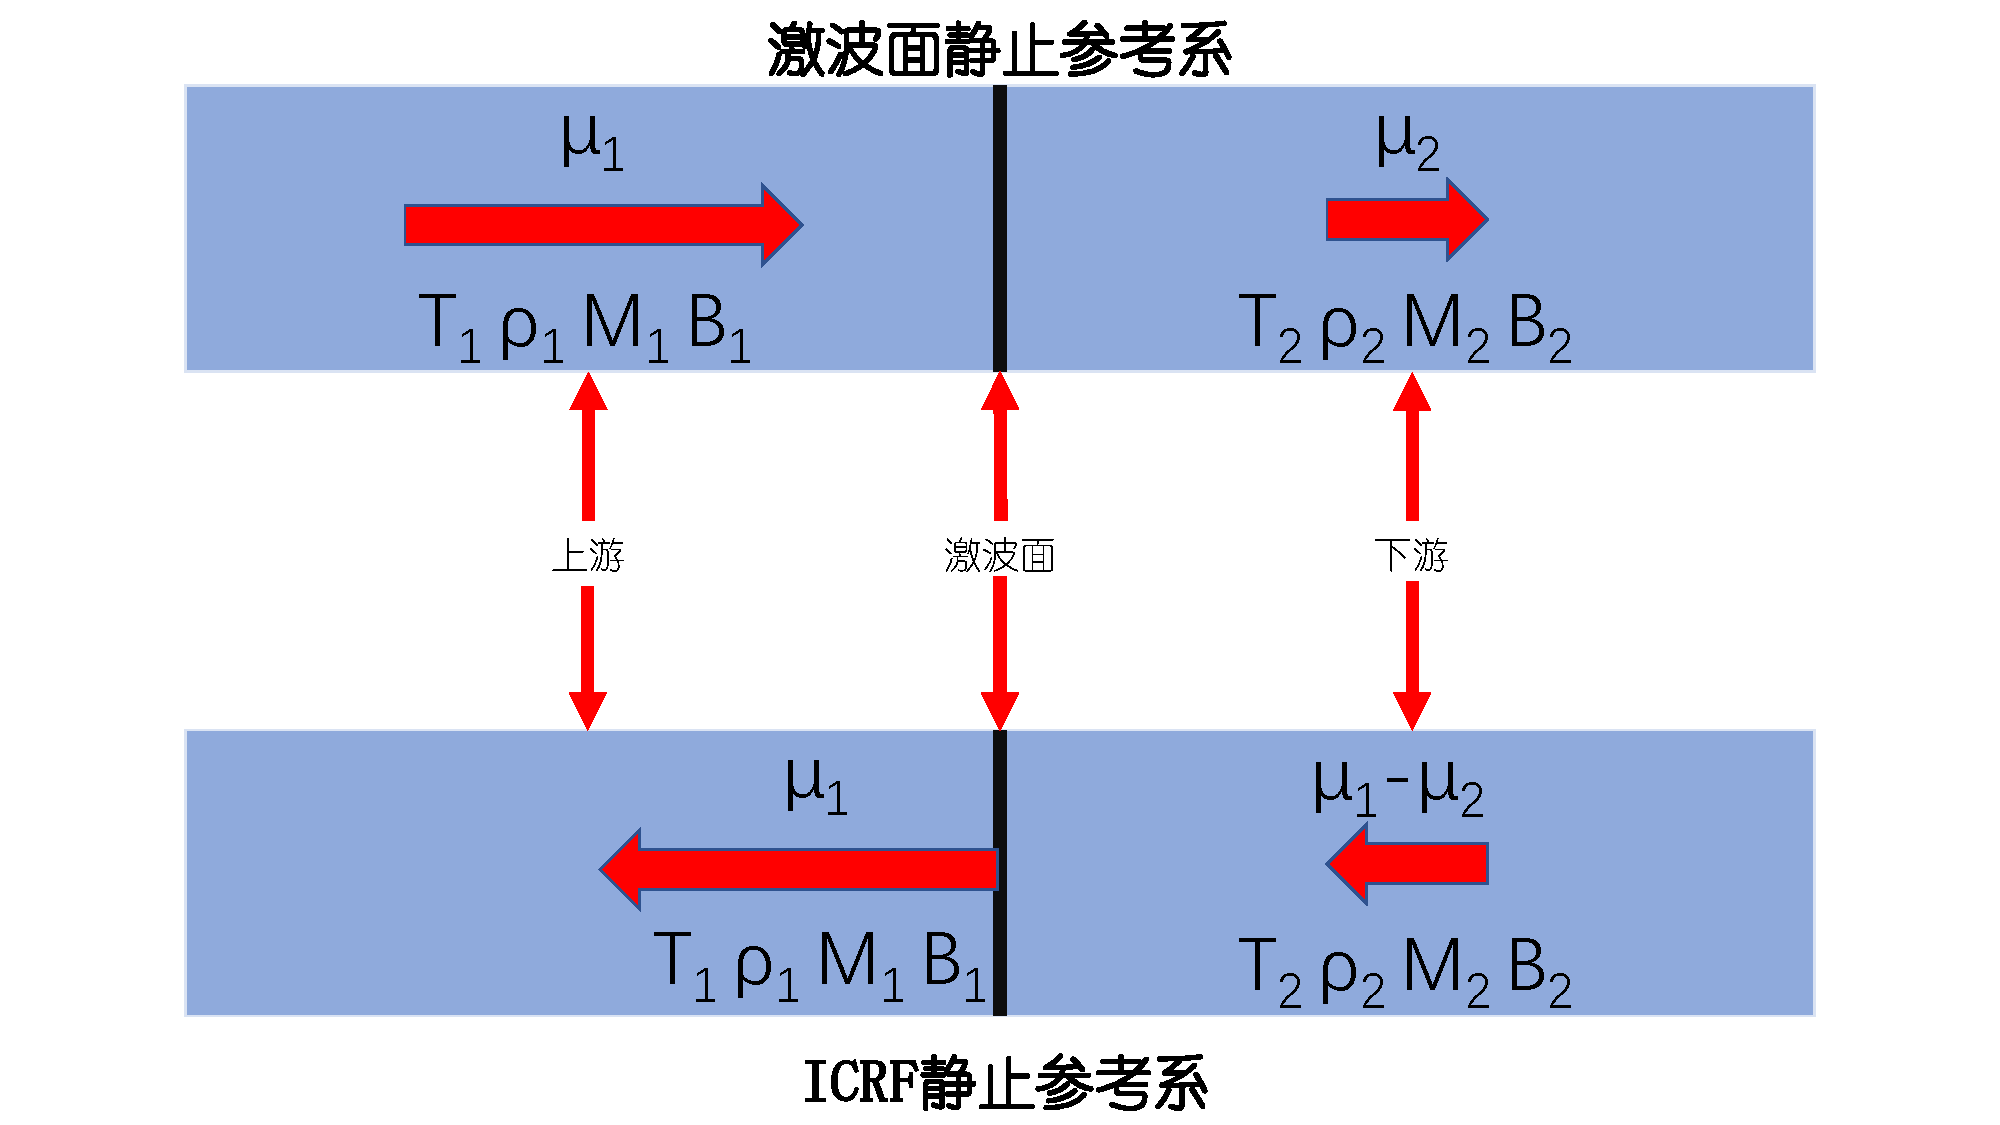
\includegraphics[width=0.9\textwidth]{ICRF.pdf}
    \caption{激波面静止参考系和国际标准参考系上下游的状态。}
\label{fig:shock}
\end{figure*}

而激波的重要特征之一就是,激波面分割开的上游和下游物理量差异很大,或者称为激波面不连续性。
取激波面为静止参考系,运动朝向激波面的为上游,速度、密度、温度、磁场、马赫数为$\mu_1$、
$\rho_1$、$T_1$、$B_1$、$M_1$,远离激波面的为下游,速度、密度、温度、磁场、马赫数为
$\mu_2$、$\rho_2$、$T_2$、$B_2$、$M_2$,如图~\ref{fig:shock}。
要注意,这里并没有抛射物混入,所以上下游其实都是原本就存在的ISM或者CSM,因而应该满足质量
守恒$\rho_1\mu_1=\rho_2\mu_2$,这里我们定义压缩比$r=\rho_2/\rho_1=\mu_1/\mu_2$。
而这里的动量守恒可粗略写为$\rho_1\mu_1^2=\rho_2\mu_2^2$,我们知道压强其实就是运动粒子
的动量造成的,这里的动量其实就是动压。
而热压在这里其实也是不可忽略的,所以准确的动量守恒方程应该为
$\rho_1\mu_1^2+p_1=\rho_2\mu_2^2+p_2$。
这里我们忽略了磁场,而遗迹当中磁压其实也很重要,考虑进来的话可得
$\rho_1\mu_1^2+p_1+B_1^2/8\pi=\rho_2\mu_2^2+p_2+B_2^2/8\pi$。
不过在这一节的讨论中,我们不考虑磁压,更多关于磁压的讨论请见章节~\ref{TheoryMHD}。


因为$c_{s}^{2}=\gamma p/\rho$,故不考虑磁压的动量守恒方程改写为

\begin{equation}
  \begin{aligned}
    \rho_{1} \mu_{1}^{2}\left(1+\dfrac{p_{1}}{\rho_{1} \mu_{1}^{2}}\right)=
    \rho_{1} \mu_{1}^{2}\left(1+\dfrac{c_{s, 1}^{2}}{\gamma \mu_{1}^{2}}\right)=
    \rho_{1} \mu_{1}^{2}\left(1+\dfrac{1}{\gamma M_1^{2}}\right).
  \end{aligned}
\end{equation}

假设在国际标准参考系中(International Celestial Reference Frame,ICRF)激波上游介质在SNR
演化时标内可看作是静止的,如图~\ref{fig:shock},我们在激波面的静止系中看到的$\mu_1$
其实就是激波面本身的速度,$M_1$与$M$其实是一个量。
而$M\gg 1$,所以近似得$\rho_1\mu_1^2+p_1=\rho_1\mu_1^2$,
也就是$\rho_1\mu_1^2=\rho_2\mu_2^2+p_2$,两侧除以$\rho_2\mu_2^2$可得

\begin{equation}
    \begin{aligned}
       \dfrac{\mu_{1}}{\mu_{2}}=1+\dfrac{p_{2}}{\rho_{2} \mu_{2}^{2}}
       =1+\dfrac{1}{\gamma M_{2}^{2}} \ ,
    \end{aligned}
\end{equation}

如果取单原子气体绝热指数$\gamma$=5/3,可得$r=1+3/(5 M_{2}^{2})$。

能量守恒方程类似,$0.5\rho_1\mu_1^3+\rho_1\mu_1\epsilon_1+p_1\mu_1=
0.5\rho_2\mu_2^3+\rho_2\mu_2\epsilon_2+p_2\mu_2$,
理想气体中,$\epsilon=p/\rho/(\gamma-1)$,所以可得:

\begin{equation}
    \begin{aligned}
      \dfrac{1}{2}\rho_1\mu_1^3+\dfrac{\gamma}{\gamma-1}p_1\mu_1=
      \dfrac{1}{2}\rho_2\mu_2^3+\dfrac{\gamma}{\gamma-1}p_2\mu_2\ ,
    \end{aligned}
\end{equation}

同样因为$M_1\gg 1$,所以两侧除以$0.5\rho_2\mu_2^3$,可得$r^2=1+3/(M_{2}^{2})$。
与$r=1+3/(5 M_{2}^{2})$联立解方程组可得$r=4, M_{2}^{2}=0.2$。

激波上游主要是介质构成,而激波下游主要是受到SNR激波影响。
根据这个推导,我们可以通过介质和激波的性质,估计受到影响后的介质性质。
比如:

\begin{equation}
    \begin{aligned}
      \dfrac{1}{5}=M_{2}^{2}=\dfrac{\mu_{2}^{2}}{c_{s, 2}^{2}}=
      \dfrac{\mu_{1}^{2}}{16 c_{s, 2}^{2}}=\dfrac{\overline{m} \mu_{1}^{2}}{16 \gamma k T_{2}}\ ,
    \end{aligned}
\end{equation}

因而可得$k T_{2}=3/16 \overline{m} \mu_{1}^{2}$。
如果取H质量丰度为0.707,He质量丰度为0.274,其余粒子平均原子量为20,再考虑电子则平均粒子
权重为0.64。
则$\overline{m}$使用约化质量后得$k T_{2}=1.3 \times 10^{-6}(\mu_1/(km/s))^2 keV, T_2 =
15 (\mu_1/(km/s))^2 K$。
另外$p_2$和$\rho_2$也可以据此推出,这可以帮助我们理解很多SNR演化的细节,比如不同位置
的X射线辐射特征。

要注意,在这个推导过程中,我们用了很多假设:理想气体假设、强激波假设、介质静止假设、
单原子气体假设、无磁场假设。
这个无磁场假设是最有可能造成问题的,接下来我们要讨论DSA的核心部分,这一部分使用了上面
的推导结果,却又必须考虑磁场进行下一步分析。
问题是,我们下一步对磁场的讨论中,假设磁场对上面已经导出的结果影响不大。
可是实际上,在之前的推导过程中已经提到过磁场会影响动量守恒方程,当然,也将影响能量守恒方程。
不过,经典的DSA推导就是这么做的,所以我们也先接受这个简化模型。

之前的推导都是基于激波面静止坐标系,下面换个坐标系讨论。
设$\mu=\mu_1-\mu_2$,则
在上游静止坐标系中看,也就是国际标准参考系中看,激波面的速度为$\mu_1$,下游速度为$\mu$,
在下游静止坐标系中看,激波面的速度为$\mu_2$,上游速度为$\mu$。
在上游静止坐标系中看,下游在朝上游移动,上游总会有一个相对上游静止的粒子来到下游。
之后,这个粒子与等离子体中的带磁场的团块(简称磁块)相互作用,这些团块其实是等离子体的集合体,
在上游静止坐标系中看以速度$\mu$朝上游运动。
而这个来到下游的粒子受到团块磁场偏转,类似于完全弹性碰撞,下游整体相对于粒子是质量极大
物体,根据完全弹性碰撞公式

\begin{equation}
    \begin{aligned}
      v_{small}^{\prime}=\dfrac{\vec{\bold{V}}_{small}\left(m_{small}-m_{large}\right)+2
      m_{large} \vec{\bold{V}}_{large}}{m_{large}+m_{small}}\ ,
    \end{aligned}
\end{equation}

粒子获得下游整体速度的两倍,然后来到上游。
这时候这个原本在上游静止坐标系中看来静止的粒子拥有了$2*\mu$的速度。
还是在上游静止坐标系中看,上游整体相对于粒子是质量极大物体,粒子以原速率反弹,也就是以
速度$2*\mu$进入下游。
类似于第一次循环,粒子获得下游整体速度的两倍,然后来到上游。
这时候这个原本在上游静止坐标系中看来静止的粒子拥有了$4*\mu$的速度。
平均每经过一次激波面,这个粒子就获得$\mu$的速度。
要知道,上游静止坐标系其实就是介质所在的坐标系,在SNR演化过程中基本可以认为就是静止,
所得的速度基本就是真实速度。
个人在将其中的粒子与磁块相互作用类比于完全弹性碰撞,细微之处或许略有不妥,但相对
来说简单理解,而推导结果也是没问题的。

虽然上游的粒子肯定会跑到下游,可是下游的粒子如果速度不够快,可能就追不上激波面,最终
远离加速区。
可实际上,经过一次循环加速,速度就达到了$2*\mu$,由$r=4$可知粒子速度已经远超过了下游速度,
所以基本不存在追不上激波面这种情况。
所谓逃逸的粒子多是由于磁场存在,在下游区域不断做回旋运动,虽然自身速度很高,但是
最终结果是随着下游整体在运动,而后慢慢脱离加速区。
所以说,下游粒子回到上游并不是因为自己速度很快,而是更类似于粒子扩散过程,这也是DSA
名称的由来。

经过讨论我们也发现,其实我们加速的粒子都是一开始周围介质的粒子,如前文所讲,超新星的抛射物
本身大部分没有参与到加速中。
当然我们在这里没有考虑反向激波,那又是另一个话题了。
所以下面要开展的能谱讨论里,我们只关注上游粒子。
此外,各种粒子实际上都有很高的初始速度,有一些甚至已经是相对论化的,直接根据上面定性
的推导计算获得的能量肯定不妥,所以要有更精确的计算。

设在上游静止坐标系上游粒子初始能量为$E$,初始动量为$p$。
考虑粒子经过激波面的入射方向与激波面法线夹角为$\theta$,而激波如果是相对论化的要再加一个
洛伦兹因子$\gamma_\mu$,这样,在下游静止坐标看这个粒子能量为
$E^{\prime}=\gamma_{\mu}(E+p \cos (\theta)\mu )$。
如果激波是非相对论的($\gamma_{\mu}=1$),而粒子是相对论化的($E=pc$),那么

\begin{equation}
    \begin{aligned}
      E^{\prime}=E+\dfrac{E}{c} \mu \cos (\theta)\ ,
    \end{aligned}
\end{equation}

从上游进入下游获得的能量就是

\begin{equation}
    \begin{aligned}
      \dfrac{\Delta E}{E} = \dfrac{\mu}{c} \cos (\theta)\ ,
    \end{aligned}
\end{equation}

反之亦然。

之前一直在讨论单个粒子,而能谱分布是相对很多粒子而言的。
假设不同方向粒子是均匀的,那么$\theta$到$\theta+d\theta$范围内的入射的粒子数与
$\sin(\theta)d\theta$成正比。
而很显然,垂直入射穿过激波面的概率为1,而平行入射几乎无法穿过激波面,那么粒子穿过激波面
的概率与$\cos(\theta)$成正比。
那么,如果有一群相同粒子之中,其中每一个都有可能以
$p(\theta)\propto \cos(\theta)\sin(\theta)d\theta$的概率穿过激波面。
总的穿过概率当然是1,那么有

\begin{equation}
    \begin{aligned}
      A \int_{0}^{\frac{\pi}{2}} \mathrm{d} \theta \cos
      (\theta) \sin (\theta) \equiv 1\ ,
    \end{aligned}
\end{equation}

解得A=2,所以$p(\theta)=2\cos(\theta)\sin(\theta)d\theta$。
这样总体粒子穿越一次激波面的平均能量获取就是

\begin{equation}
    \begin{aligned}
      <\dfrac{\Delta E}{E}>=\frac{2\mu}{c} \int_{0}^{\frac{\pi}{2}}
      d \theta \cos ^{2}(\theta) \sin (\theta) = \dfrac{2\mu}{3c} \ .
    \end{aligned}
\end{equation}

也就是说,粒子经过一次从上游到下游再回到上游,能量变为原来的$(1+4\mu/3c)$倍,
可见这是个一阶加速机制。

取$\beta_a=(1+4\mu/3c)$,而$P$为每个循环后仍留在加速区的可能性且为常数,设$N$为能量高于$E$的
粒子数,循环$k$次后可得

\begin{equation}
    \begin{aligned}
      N(>E)=N_{0} P^{k}\ ,\  E=E_{0} \beta_a^{k}\ .
    \end{aligned}
\end{equation}

取对数后相除得:

\begin{equation}
    \begin{aligned}
      \dfrac{\log \left(N(>E) / N_{0}\right)}{\log \left(E / E_{0}\right)}=
      \dfrac{\log P}{\log \beta_a} \ ,
    \end{aligned}
\end{equation}

也就是:

\begin{equation}
    \begin{aligned}
      N(>E)=N_{0}\left(\dfrac{E}{E_{0}}\right)^{\frac{\log P}{\log \beta_a}} \ ,
    \end{aligned}
\end{equation}

微分后可得:

\begin{equation}
  \label{eqn:SED}
    \begin{aligned}
      n(E) \propto E^{-1+\frac{\log P}{\log \beta_a}} \ .
    \end{aligned}
\end{equation}

这可以说就是一个幂律谱的能谱方程,可是我们目前不知道其谱指数,因为P还是未知量。
好在,我们知道每个循环中粒子逃逸的概率是(1-P),而这个概率是可以计算的。
设单位时间离开、进入加速循环的粒子数分别为$R_{out}$和$R_{in}$,则
$R_{out}/R_{in}=1-P$。
然后设$n$为加速区加速粒子的密度,如果密度均匀,则有:

\begin{equation}
    \begin{aligned}
      dn=\dfrac{n}{4 \pi} d \Omega \ ,
    \end{aligned}
\end{equation}

设粒子穿越激波面的速度为$v_p\cos(\theta)$,可得

\begin{equation}
    \begin{aligned}
      R_{i n}=\int_{u p \rightarrow d o w n} v_p \cos (\theta) d n =
      \dfrac{n v_p}{4 \pi} \int_{0}^{\frac{\pi}{2}} \cos (\theta) \sin (\theta)
      d \theta \int_{0}^{2 \pi} d \psi=\dfrac{1}{4} n v_p \ .
    \end{aligned}
\end{equation}

如果认为逃逸的粒子大部分来源于下游自然流出,那么$R_{out}=n\mu_2$。
也就是说$1-P=4n\mu_2/nv_p=\mu_1/v_p$,通常粒子入射速度很高,可以认为$\mu_1/v_p \ll 1$,
这说明大部分粒子都经过多次循环。
即使在介质区物质集体状态基本静止,单个粒子速度还是很快的,甚至大部分接近光速,可取$v_p=c$。
当然如果激波速度太快,而粒子初始速度太慢,那可能很快就被抛出加速区了。

目前为止,我们可以得到$P=1-\mu_1/c$,$\beta_a=(1+4\mu/3c)=1+\mu_1/c$。
再看方程~\ref{eqn:SED},其中

\begin{equation}
  \label{eqn:index}
    \begin{aligned}
        \begin{cases}
          \log P=\log \left(1-\dfrac{u_{1}}{c}\right) \sim-\dfrac{u_{1}}{c} \ , \\

          \log \beta_a=\log \left(1+\dfrac{u_{1}}{c}\right) \sim \dfrac{u_{1}}{c} \ , \\
        \end{cases}
    \end{aligned}
\end{equation}

然后可得

\begin{equation}
  \label{eqn:spec}
    \begin{aligned}
      n(E) \propto E^{-2} \ .
    \end{aligned}
\end{equation}

这就是由DSA机制刚好可得出的加速粒子幂律谱,是一个非常棒的结果,一经提出便被广泛认为是
SNR中产生同步辐射的相对论电子的基础。
当然我们不要忘了这个计算结果其实是基于很多假设的。
在推导激波及上下游性质时,我们已经提到了一些假设。
而在推导粒子加速时,我们又引入一些新的假设:弹性碰撞假设、激波非相对论假设、粒子相对论化
假设、粒子各向同性假设、非线性效应可忽略、忽略其它逃逸方式。
每一个假设不成立,都会导致谱指数的改变。
比如经常出现激波并不是强激波,那么$r\neq4$,结果只能用
$P=1-4\mu_2/c$,$\beta_a=(1+4\mu/3c)\neq1+\mu_1/c$。
类似方程~\ref{eqn:index},可得

\begin{equation}
    \begin{aligned}
      n(E) \propto E^{-\frac{r+2}{r-1}} \ .
    \end{aligned}
\end{equation}

可见激波越弱,谱指数越大,谱越陡。
另外,磁场的存在也会使得谱指数变大,具体推导见章节~\ref{TheoryMHD}。
同时,周围介质其实并不一定是静止的,比如前身星本身有高速运动,那么相当于介质存在一定速度,
这样SNR不同方向激波中的加速效率$\beta_a$也是不一样的,这也是SNR壳层亮度不同的一个原因。

此外,我们在这里都是忽略了辐射损耗的,然而,高效的激波加速会导致更严重的辐射损耗。
同时,大量的高能相对论粒子会缩小绝热系数$\gamma$。
这两个效应都可能增大压缩系数$r$\citep{Ellison2005},而且相关观测也发现SNR中有的位置
压缩系数可能被增大\citep{Voelk2007}。
这些条件会使得谱指数变小,谱变平,最终我们看到的粒子分布是各种效应叠加的结果。



\subsection{宇宙线起源}
自从\citet{hess1912beobachtungen}发现宇宙线以来,这一领域一直受到人们的广泛关注,而
对其起源的猜测也从未间断\citep{Reynolds2008a}。
不过,随着近几年高能观测的增多,SNR对银河系宇宙线有很大贡献已经成为一个不争的事实
\citep{Ackermann2013, Joubert2016, Jogler2016}。
当然诸如脉冲星风云(Pulsar Wind Nebula, PWN)和黑洞的贡献应该也需要考虑
\citep{Abeysekara2018, Profumo2018}。
不过,测量的宇宙线能谱,在考虑传播过程后需要一个能产生谱指数为-2的幂律分布
粒子的机制来解释,虽然SNR刚好满足这一条件,但其实我们推导的DSA产生的能谱只是加速区的能谱,
加速区中的粒子释放到ISM中的时候会经历冷却、或者反向激波再加速等过程,最终的谱指数很可能
不是-2。
所以说,我们对宇宙线能谱仍然不甚了解,除了这个粒子释放的问题,还有一直难以理解的“膝区”
\citep{Hoerandel2003}。
而对其解释其实有很多,很自然的想法就是加速源有两种,加速产生的能谱不同。
但具体这两种是什么,会不会多种的贡献互相叠加,我们还不是很清楚。

我们可以先尝试了解SNR对宇宙线能谱的贡献\citep{Ptuskin2010},这样我们不仅需要
知道其谱指数,还需要得到能谱截断能量,也就是SNR能将例子加速到的最大能量$E_{\max}$。
这个也可以由DSA来估计。
我们知道下游粒子来到上游再回到下游这个循环中,其实主要影响粒子宏观运动的是扩散效应。
这里引入扩散系数$D$,假设粒子从下游进入上游后,跑了$t_d$的时间到达距激波面最远处,然后
与追上来的激波面接触并进入下游,这个最远处与激波面距离为$l_d$,可得
$l_{d} \approx \sqrt{D t_{d}}$。
当然,我们也有$l_{d}=u_{1} t_{d}$,解得$t_d \approx D/\mu_1^2$。
扩散系数其实是与粒子的能量有关的$D=D_{0} E^{\alpha}$,能量越大,扩散系数越大,
而$l_{d}$、$t_{d}$也就越大,多次加速后会超出加速区范围。
这其实是另一种粒子逃逸方式\citep{Li2012},但相比于直接从下游流走的粒子数要少,所以在
DSA推导时没有考虑。

这里可见,一次循环的加速时标近似于$t_{d}$,假设最多可经历$m$次循环,那么所得最高能量为
$E_{\max }=(u_{1}^{2} m t_{d}/D_{0})^{1/\alpha}$。
根据类似思路,\citet{1983A&A...125..249L}估算出SNR最多能加速粒子到100TeV,而膝区位置
都是大于1PeV的,这个$E_{\max}$远远不够。
\citet{Zirakashvili2018}将磁场考虑在内,并尝试加入一个前身星星风吹出的壳层来放大初始
介质磁场,从而提高截断能量。
而我们也尝试通过模拟来检验这件事,并证实了这种思路的可行性\citep{Zhang2018}。
不过,目前对这个模型的观测支持其实并不多,因为我们观测到遗迹时其前身星星风早已被激波
冲散,很难得到直接证据,或许对年轻的遗迹周边进行观测能够帮助我们确切证实这件事。

\subsection{SNR中的辐射机制}

除了很早就有人意识到的DSA加速的电子会产生同步辐射,且射电谱指数$\beta$与电子分布谱指数$\eta$
存在关系$\beta=(\eta-1)/2$,
\citet{Reynolds1981}提出类似的机制也可以产生非热的X射线辐射,而他们发现SN 1006
就是一个很好的例子\citep{Becker1980},可是这要求粒子加速能量远超过100TeV,
在当时来看是不太可能的。
后来,\citet{1982ApL....22..103G}接近1keV的能段发现了X射线的谱线,所以大家都认为
SN 1006也是热谱,无法作为产生X射线非热谱的例子。
然而,更高空间分辨率的观测显示,这个SNR壳层区的确是非热的,中心区才是有谱线的
\citep{Koyama1995},所以事情又反转了。
后来,\citep{Reynolds1998}通过改进自己之前的模型,发现即使粒子截断能量在100TeV也能
很好拟合SN 1006的X射线能谱。
这个工作说明了两件重要的事情,DSA产生的相对论电子的确可以通过同步机制产生X射线非热辐射,
同时可知,DSA的确可以将粒子加速到100TeV,我们对DSA的推导是正确的。

除了主要产生同步辐射的高能电子,稍微低能一些的非热电子会通过韧致辐射产生能量范围从keV
到TeV的光子。
所有电子都会通过与各种原子核相互作用产生韧致辐射。
热电子只会产生一般的热连续谱辐射,而能量较高的非热电子则通过同步辐射产生幂律谱的同时
也会通过韧致辐射产生幂律谱。
通常一个能量为$E$的电子经过韧致相互作用会释放能量大约为$E/3$的光子,可是同步辐射并不会
有这么高的能量转化,结果就是能量为TeV的电子,可能通过韧致辐射产生TeV光子,但通过同步
辐射只能最高产生keV的光子。
另外,其实如果电子能量很高,互相之间也会产生韧致辐射,有时在拟合能谱时是不可忽略的。

高能电子本身会散射背景光子场,比如宇宙微波背景辐射(Cosmic Microwave Background,
CMB),然后产生能量能达到TeV的光子,这就是逆康普顿散射。
背景场可能有很多种,SNR自身产生的射电辐射、星系自身的背景辐射等有所贡献。
真正在拟合能谱时,甚至要考虑附近大质量恒星的辐射。

此外,高能质子相互作用可能产生$\pi^0$介子,$\pi^0$介子衰变成的$\gamma$光子能量也很高。
不过这种情况在SNR本身的环境中很难发生,因为这要求很高的质子密度。
而当SNR周围刚好存在分子云,激波与分子云相互作用时就会产生非常不一样的能谱。
之前观测上已经有很多证据表明电子在SNR中被加速至高能,但是这些其实无法说明质子是否也被加速。
可我们观测到的宇宙线主要由质子组成,电子因为在磁场中运动辐射能量很快,无法保持高能到达地球,
宇宙线的能谱也主要也是由质子所贡献。
所以说,观测到质子在SNR中加速才能说明SNR是宇宙线的起源地。
而通过观测激波与分子云相互作用时产生的与电子辐射的不同的能谱,我们可以确定的确有高能质子
的存在,这才真正证实SNR是部分宇宙线的来源地。



\section{磁流体模拟基础}
\label{TheoryMHD}

\subsection{磁场的重要性}
前述DSA的推导中我们都忽略了磁场,不然动量守恒方程应该是
$\rho_1\mu_1^2+p_1+B_1^2/8\pi=\rho_2\mu_2^2+p_2+B_2^2/8\pi$。
现在我们来讨论一下,磁场是不是真的不重要。
取$\rho_1=1 m_p cm^{-3}, \mu_1 = 100 km/s$,则动压
$\rho_1\mu_1^2=1.6 \times 10^{-10} dyn/cm^{2}$。
取$\B_1=9\mu G$,则磁压$B_1^2/8\pi=3.2 \times 10^{-12} dyn/cm^{2}$。
这里我们用的速度是比较小的,而磁场是比较大的。可见,磁压相对来说不重要。
不过磁场在激波与介质作用时是会放大的,我们算过压缩比$r=4$,因为磁通守恒,我们暂且
假设激波后磁场放大4倍,那么取$B_2=36\mu G$,则磁压
$B_2^2/8\pi=5.1 \times 10^{-11} dyn/cm^{2}$。
这时候磁压都达到了动压的一半,不应该忽略了。
其实考虑湍流后磁场放大到$100\mu G$现在看来已经是可能的了\citep{Ji2016b},假设放大十倍
后可取$B_2=90\mu G$,则磁压$B_2^2/8\pi=3.2 \times 10^{-10} dyn/cm^{2}$。
所以,下游的磁压其实是不能忽略的。
如果上游的磁场因为前身星星风等原因得到放大,也就不应该忽略。
总体来说,大部分情况是不能忽略磁压的,故经典DSA是存在这样一个明显的瑕疵的。

那么磁压到底对我们的DSA推导影响多大呢?
类似于DSA推导,设激波后磁场放大4倍,即$B_2=4B_1$,将考虑磁场的动量守恒方程两侧除以
$\rho_2\mu_2^2$,可得

\begin{equation}
    \begin{aligned}
      \dfrac{\mu_1}{\mu_2} = 1+\dfrac{p_2}{\rho_2\mu_2^2}+
      \dfrac{15}{16\rho_2\mu_2^2}\dfrac{B_2^2}{8\pi }\ ,
    \end{aligned}
\end{equation}

然后设热压磁压比$\beta_b=8\pi p/B^2$,可得

\begin{equation}
    \begin{aligned}
      r = 1+
      \left(1+\dfrac{15}{16\beta_{b,2}}\right)\dfrac{3}{5 M_2^2} \ .
    \end{aligned}
\end{equation}

类似的,已知能量守恒方程为

\begin{equation}
    \begin{aligned}
      \dfrac{1}{2}\rho_1\mu_1^3+\dfrac{\gamma}{\gamma-1}p_1\mu_1+\dfrac{\mu_1B_1^2}{8\pi}=
      \dfrac{1}{2}\rho_2\mu_2^3+\dfrac{\gamma}{\gamma-1}p_2\mu_2+\dfrac{\mu_2B_2^2}{8\pi}\ ,
    \end{aligned}
\end{equation}

两侧除以$0.5\rho_2\mu_2^3$,整理可得

\begin{equation}
    \begin{aligned}
      r^2 + \dfrac{3r}{40\beta_{b,2}M_2^2} = 1 + \dfrac{3}{M_2^2}
      +\dfrac{6}{5\beta_{b,2} M_2^2} \ .
    \end{aligned}
\end{equation}

联立动量守恒方程,解得

\begin{equation}
      \label{eqn:ratio}
    \begin{aligned}
        \begin{cases}
          M_2^2 = \dfrac{1}{5}+\dfrac{2}{5\beta_{b,2}}+\dfrac{1131}{256\beta_{b,2}^2} \ , \\

          r = 1 + \dfrac{3}{5M_2^2}\left(1+\dfrac{15}{16\beta_{b,2}}\right) \ . \\
        \end{cases}
    \end{aligned}
\end{equation}

可见,热压相比磁压越大,磁场部分就越不重要,最后可以回到经典DSA推导。
要注意,我们在这里直接设激波后磁场放大4倍,如果我们认为这个倍数就是压缩比$r$,那么将其
代入后$B_2=rB_1$,根据相同步骤也可推导出更准确的结果。
不过这样推导过于复杂,而且真实情况中,磁场放大机制不止介质压缩,各种不稳定性及局部湍流
都会影响放大,所以这里暂且使用这一粗略结果。

同时,$\beta_{b,2}\to \infty, r\to4$,分析可知,$r$在这里最大为4,其实即使考虑
激波后磁场放大$r$倍,计算结果也是最大为4,也就是说压缩比在强激波条件下为最大。
再与方程~\ref{eqn:spec}相比较,可知考虑磁场后的激波产生的幂律谱会更陡,不能算是强激波,
看似好像这个激波是弱的,更难将粒子加速到高能。
可实际上,粒子在强磁场中更容易驻留,同样时间内经历更多次加速循环,因而虽然谱陡,但是
加速到高能的粒子反而可能更多。
当然,这需要进一步计算,类似应用请看\citet{Zirakashvili2018}的工作。
而这个推导也可以帮助我们理解“膝区”形成,可能证实因为有的激波加速磁场很强,而有的很弱导致
谱指数的不同。
磁场很强的激波加速中,截断能量更高,可是谱很陡,而磁场很弱的激波加速正相反。
也就是说强磁场激波加速对高于“膝区”的谱贡献大一些,而弱磁场激波加速对低于“膝区”的谱贡献
大一些。
此外,这种因为磁场强度不同而导致的粒子谱指数变化自然地也会影响到同步辐射谱指数,而实际上
SNR不同区域的谱指数相差很大\citep{Leahy2005, Tian2005},我们这里讨论的因素应该也对这
一现象有很大影响。

总之,磁场对SNR的演化及粒子的性质影响很大,我们不应该将其忽略,这也是我们开始这篇文章中
工作的重要原因之一。

\subsection{磁流体特性}
说到流体,我们要提到一个最著名的假设,连续介质假设。
当我们讨论流体时,通常都默认这一假设成立,但是在某些极端情况,尤其是天文研究中,这个假设
很多时候都是不成立的。
这个假设主要就是说统计上流体中的组成粒子都可看作质点,质点间几乎不存在间隙\citep{hd}。
不过实际判定的标准分为空间和时间两个方面,这两个方面都是对我们统计粒子这一行为提出的。

首先,空间上,进行统计的粒子可看作质点,微观上足够大,宏观上足够小。也就是说,微观上粒子
尺度比粒子间空隙大得多,宏观上粒子比所研究的尺度小得多。比如研究倒一杯水,水分子比水分子
间空隙要大,水分子的尺度比杯子的尺度要小。
而时间上,进行统计粒子用的时间,在微观足够长,在宏观上足够短。也就是说,微观上时间够长,
粒子已经碰撞多次满足统计要求,而宏观上时间够短,统计粒子的时间比我们研究流体过程时间
要短。

说到这里,我们大概意识到,SNR的磁流体模拟其实是不满足连续介质假设的,主要是因为粒子间空隙
比粒子大得多。
不过,很多时候SNR中的流体是可以看作连续的,因为我们进行统计粒子用的时间甚至可以以年为单
位计算,这时候粒子间已经碰撞多次,统计上可以当作空隙很小。
其实,我们在推导DSA使用守恒方程时,已经默认了这一假设成立。
举个例子,研究时间很短,上游粒子来到下游,还没有其它粒子回到上游,统计粒子
的时间比我们研究流体过程时间要长,这时候守恒律当然是不成立的。
一般情况下,这一假设没有问题,不过要做极端讨论时就得考虑。

此外,在SNR演化过程中会存在各种不稳定性,
其中明显会出现的就是瑞利-泰勒不稳定性(Rayleigh-Taylor instability, RTI),这种
不稳定性主要发生在密度低的流体推动密度高的流体时,看起来很明显超新星爆发的抛射物与介质之
间的关系就是这样。
不过要注意的是,这种不稳定性是需要持续施力的,一旦两者之间没有加速度,我们看到的参数起伏
就不再是RTI直接导致的,而是初期RTI引起的连锁反应。
所以对于大部分SNR如果中心有PWN的持续供能,那么RTI会持续起作用,如果没有,可能RTI只是
剩下后续的扰动影响。
特别的是,RTI尤其要与里克特迈耶-梅什科夫不稳定性(Richtmyer–Meshkov instability, RMI)
区分开,这种不稳定性是在两种流体接触的位置因为局部扰动引起瞬间加速导致的,我们在磁流体
模拟中经常遇到这种不稳定性。
此外,与RTI看起刚好相反的是开尔文-亥姆霍兹不稳定性(Kelvin–Helmholtz instability, KHI),
两种流体相切接触时才会产生KHI。
虽然看起来SNR中抛射物与介质是相向接触,但实际上,因为介质密度不均匀,相切接触也是时有发生。
这些不稳定性都会导致局部参数的起伏,放大局部磁场,改变不同区域同步辐射谱指数,这才导致
我们看到的SNR内部结构千变万化。

此外,我们在推导DSA时只是研究了二维情况,三维的守恒方程要考虑更多,而且引力也是可以考虑
在内的,这里我们给出实际在磁流体模拟中使用的方程:

\begin{equation}
\frac{\partial}{\partial t} \left( \begin{array}{c}{\rho} \\ {m} \\ {E+\rho \Phi}
\\ {B}\end{array}\right)+\nabla \cdot \left( \begin{array}{c}{\rho v} \\
{m v-B B+\mathbf{I} p_{t}} \\ {\left(E+p_{t}+\rho \Phi\right) v-B(v \cdot B)}
\\ {v B-B v}\end{array}\right)^{T}=\left( \begin{array}{c}{0} \\
{-\rho \nabla \Phi+\rho g} \\ {m \cdot g} \\ {0}\end{array}\right)
\end{equation}

其中$\mathbf{I}$是单位积,
$\mathbf{I} \equiv \hat{\boldsymbol{e}}_{1} \hat{\boldsymbol{e}}_{1}+
\hat{\boldsymbol{e}}_{2} \hat{\boldsymbol{e}}_{2}+\hat{\boldsymbol{e}}_{3}
\hat{\boldsymbol{e}}_{3}$, 而${m}=\rho {v}$,$p_{t}=p+B^{2} / 8\pi$,
$E=\rho \epsilon+m^{2}/2 \rho+B^{2}/8\pi$,$\rho \epsilon=\rho \epsilon(p, \rho)$,
$\Phi$和$g$是引力势和加速矢量。
我们之前对DSA的讨论是基于二维的,三维磁流体中需要考虑磁场张量作用,在方程中体现为$BB$等
并矢。
这种张量作用会产生阿尔文波,这种波是带电粒子在垂直于磁场方向运动时,受到局部扰动时产生的
沿着磁场方向运动的波,这种波会影响局部磁场,导致不同位置的粒子加速情况有所不同,与上面
提到的三种不稳定性一起改变不同区域同步辐射谱指数。
因为我们实际进行的磁流体模拟是三维的,所以在程序编写中是对其有所考虑的。
当然,我们之前的讨论也忽略了引力,这个忽略与忽略磁场不同,对SNR来说是非常合理的。
此外,虽然我们这里的方程写得很正确,但是数值计算时可能依旧会有问题,比如磁场无源其实就
无法保证,因而与物理事实其实还是有些差别。
不过经过改进算法,我们可以克服这些问题。

\chapter{使用PLUTO进行磁流体模拟的程序编写}
\label{PLUTO}



\section{PLUTO软件简介}
\label{PLUTOintro}
PLUTO是一个有多国科研人员共同完成的流体模拟软件,至今为止一直得到很好的维护,是进行天体
物理相关模拟的可靠软件\citep{Mignone2007,Mignone2012}。
目前,软件只支持Linux/Unix平台运行,最基本的运行只依赖Python2、C、GNU make,几乎是每个
Linux/Unix平台发行版都会自带的。
而进一步的需求依赖不同,要进行并行计算需要安装MPI library,要输出HDF5格式需要安装HDF5
library,要进行自适应网格(Adaptive Mesh Refinement, AMR)模拟需要安装C++、Fortran和
Chombo library,HDF5 library。
当然,如果要直接输出PNG格式图像,需要安装PNG library,但是我们很少这样做,因为输出数组
格式的二进制文件后可以直接用Python读取进行可视化,结果修改更灵活。

其主题文件目录结构包括:

\begin{enumerate}

    \item Config/:包含系统配置文件,软件要根据其中的内容读取依赖的代码的信息,比如系统是否
    已经安装C,HDF5 library等。这个文件夹中原始文件都是一些针对不同系统的模板,代码编译
    之前,需要根据模板自己编写适合自己系统的配置文件。

    \item Doc/:软件文档,包括pdf文档和html文档,两者内容相差不大,pdf文档更为全面,
    html文档更为直观,html文档还有一个好处是其中的代码可以直接复制用来测试。

    \item Lib/:额外需要的运行库的安装位置。比如要进行AMR模拟,需要安装Chombo库,那么
    相应的库最好安在这个,如果安在别的地方需要额外的路径配置。

    \item Src/:程序主目录,除了初始条件设定部分,所有进行具体运算的代码都在这个目录。

    \item Tools/:有用的小工具。我们主要使用其中的pyPLUTO进行可视化。

    \item Test\_Problems/:包含各种各样使用PLUTO的例子。这些事例对于初学者非常友好,根据
    文档可直接运行,对于了解整个软件的使用很有帮助。

\end{enumerate}

而实际进行模拟时基本不需要修改这其中的文件,可以直接在自己新建的文件夹中操作,在程序运行
时设置好环境变量就行。

PLUTO本身可进行的模拟种类非常多,而本章节只以超新星遗迹模拟为例详细介绍MHD模拟方法,
而可视化方法中只介绍Python的使用与优化,更多的内容请见PLUTO的Doc目录中的官方文档。

\section{PLUTO基本使用}
\label{PLUTOuse}
具体下载安装请见http://plutocode.ph.unito.it,而在文档的Quick Start部分有简要的路径
配置,我们只介绍文件编写和运行。
软件安装、配置完成后,我们需要新建工作目录,比如目录SNR/,而要进行一个完整模拟,这个目录
中至少需要三个文件definition.h、init.c、pluto.ini。
其中definition.h主要定义需要的物理及计算方式,init.c定义初始条件,pluto.ini定义需要的
参数,三者名称都可以改变,但是个人建议使用此默认命名,之后交流比较方便。

而大概使用步骤如下:
\begin{enumerate}

    \item definition.h编写完成后,使用python \$PLUTO\_DIR/setup.py,确认使用的参数,然后选择自己
    在Config/中设置好的配置文件,如果使用Ubuntu等Linux系列平台进行非并行运算,选择默认的
    Linux.gcc.defs即可。

    \item init.c编写完成后,使用make编译程序,程序会根据definition.h中设置的参数进行编译,默认会
    生成名为pluto的可执行程序。

    \item pluto.ini编写完成后,使用./pluto运行程序,pluto程序会从pluto.ini中读取相应的数值,然后
    开始运行,运行结果与具体参数设置有关。

\end{enumerate}

\subsection{definition.h的编写}
\subsubsection{基本选项}

PHYSICS选项,定义需要的物理,可选HD(流体)、MHD(磁流体)、RHD(相对论流体)、
RMHD(相对论磁流体),我们主要介绍磁流体模拟,选MHD即可。
MHD模拟内核主要是通过解质量守恒、动量守恒、能量守恒和磁通守恒方程获得结果,需要注意的是,
这里的压强和能量包括磁压和磁能,要根据物态方程获得温度等信息时,要记得与温度有关的压强是
要扣除磁压的。

DIMENSIONS选项,定义模拟的空间维度,可选1、2、3,如果要进行三维模拟,选3即可。
COMPONENTS选项,设置矢量的分量个数,通常三维空间的矢量有三个分量,但有时为了计算方便也
可以约简其中一个分量,比如模拟恒星盘的形成时,大部分物质都在二维平面上运动,但其运动也会
影响第三维上的动量等参数。通常我们取DIMENSIONS=COMPONENTS即可。

GEOMETRY选项,设置使用的坐标系,可选CARTESIAN(笛卡尔)、CYLINDRAICAL(柱坐标)、
POLAR(极坐标)、SPHERICAL(球坐标)。
不同的坐标对不同的积分方式兼容性不同,一半情况下,选用笛卡尔坐标系即可。

BODY\_FORCE选项,可选POTENTIAL(标量势)、VECTOR(矢量引力)、POTENTIAL+VECTOR
(标量+矢量描述)。
标量势计算方便,但是在不够准确,尤其是引力场较复杂的时候。矢量引力计算时间长很多,但更准
确。我个人没有遇到过必须两者都考虑的情况,不过测试时间与只考虑矢量引力差不太多。

COOLING选项,可选POWER\_LAW、TABULATED、SNEq、H2\_COOL、MINEq。
光学薄的情况下,韧致辐射等过程导致的辐射能量损失也会影响MHD模拟结果,这个过程与当地密度、
温度、各种成分的丰度有关,尤其是丰度部分很难估算,因而模型很多。
POWER\_LAW模型是假设辐射损失与$\rho^2T^{\alpha}$成正比,其中$\rho$为密度,T为温度,
$\alpha$为幂律指数。
TABULATED模型是假设辐射损失与$n^2\Lambda(T)$成正比,其中$n$为数密度,$\Lambda$为冷却
方程,而冷却方程又有很多种\citep{2017RMxAA..53..385F}。
SNEq模型主要考虑了中性氢原子的辐射,同时也将16种最常见的谱线辐射考虑在内,比如Ly$\alpha$、
H$\alpha$、HeI、CI、OII、FeII等。
H2\_COOL模型在SNEq模型的基础上考虑了分子氢和离子氢,此外,可根据需要加入一氧化碳(CO)、
羟基(OH)和水分子(H$_2$O)等辐射贡献。
MINEq模型在SNEq模型的基础上考虑了更过谱线辐射,总共达到28种,不过对分子类辐射贡献的计算
支持不好。
超新星遗迹的模拟中,早期自由膨胀相和绝热膨胀相辐射耗散相对总能量很小,对整体模拟结果影响
不大,随着年龄变老,辐射能量越来越大,直到辐射相已经不可忽略。

RECONSTRUCTION选项,可选FLAT、LINEAR、WENO3、LimO3、PARABOLIC,是五种重构方法。
重构是模拟中的一个重要过程,随着时间变化,每一个步长间隔都需要重构一次整个模拟图像。
更好的重构方法可保证模拟结果更加准确,通常使用默认的LINEAR方法即可,如果速度太慢可尝试
FLAT方法,如果设定初始物理参数很极端而结果明显存在问题,可尝试其它三种方法。

TIME\_STEPPING选项,可选EULER、RK2、RK3、CHARACTERISTIC\_TRACING、HANCOCK,是五种
时间推演方法。
要知道,布置邻近格点会影响一个格点下一步的数值,可能更远的格点也会影响,如果步长过长,
会有过多格点影响到一个格点的数值,计算结果容易有偏差,当然,步长过短会导致运行过慢。
所以我们要选择合适的推演方法,通常在超新星遗迹模拟中选择RK2即可。
此外,我们可以通过设定Courant-Friedrichs-Lewy(CFL)数来控制具体方法,具体设定不只与
TIME\_STEPPING有关,还要考虑所选维度及是否使用DIMENSIONAL\_SPLITTING。

DIMENSIONAL\_SPLITTING选项,可选YES或者NO。
有时候,虽然我们模拟的是多维的图像,但是不同维度的影响并不会耦合,结果就是我们可以当作
在不同方向上都做一维的模拟,这时候可选YES。
而超新星遗迹的模拟每个方向上的演化都是互相影响的,所以必须选NO,不然结果很容易出错。

NTRACER选项,这其实是一个扩展选项,最大数目为4。
通常对于特定的PHYSICS守恒量都是一定的,如果要增加新的守恒量就要添加在这里,比如加入
氢原子数目守恒。

USER\_DEF\_PARAMETERS选项,输入需要的自定义参数数目,最大31。
设置初始条件时需要很多参数,比如超新星爆发能量、前身星质量、介质平均密度等,将来调参调的
就是这些,而这里只是提前设置好参数数目。

\subsubsection{物理依赖选项}
BACKGROUND\_FIELD选项,如果设置为YES,意味着设置磁场包含背景的静态场和随时变化的磁场。
超新星遗迹当中的磁场并不需要分成分,都是随时变化的,因而设为NO即可。
可是,如果需要考虑脉冲星风云中几乎保持不变的中子星磁场,就要设置为YES。

DIVB\_CONTROL选项,可选NO、EIGHT\_WAVES、DIV\_CLEANING、CONSTRAINED\_TRANSPORT。
数值方法无法保证磁场无源,我们需要强制控制其散度为零。
超新星遗迹模拟中使用EIGHT\_WAVES即可。

EOS选项,选择需要的物态方程,可选IDEAL、ISOTHERMAL、PVTE\_LAW、TAUB。
超新星遗迹的模拟中,使用IDEAL即可。

ENTROPY\_SWITCH选项,可选NO、SELECTIVE、ALWAYS、CHOMBO\_REGRID。
保证熵增原则,只对EOS为IDEAL和TAUB适用,不过在超新星遗迹模拟中影响不大,设为NO。

RESISTIVITY、VISCOSITY、THERMAL\_CONDUCTION选项,可选NO、EXPLICIT、SUPER\_TIME\_STEPPING,
控制电磁阻力、粘滞相应、热传导影响,都是有关耗散效应,在年轻超新星遗迹模拟中影响不大,
一般设为NO即可,而对老年超新星遗迹需要具体分析。
我们在章节~\ref{SW}有讨论热传导的影响,最终结论只是对星风演化影响很大。

ROTATING\_FRAME选项,使用CYLINDRAICAL(柱坐标)、POLAR(极坐标)、SPHERICAL(球坐标)
时建议选YES。

\subsubsection{自定义参数和常数}
自定义参数即是根据USER\_DEF\_PARAMETERS选项中设置的数目在这里列出相应数量的参数,而其
具体数值主要在pluto.ini中给出,然后由init.c中写的初始条件融入到整个程序里。

而自定义常数主要是一些只在特定模拟中有意义的数值,同时,编写init.c时需要控制的条件也可以
写在这里,比如设置自定义参数ADD\_TURBULENCE为YES或者NO,而init.c中有相应的条件语句从而
实现不同的功能。
其实大部分物理上的常数已经包含在不过这一部分有一个重要的功能就是设定单位制。
我们知道常用的国际单位制、CGS单位制要表达一些比较大的数值时需要科学记数法,可是在进行
模拟时这种记数法是没用的,当数值非常大或者非常小,超过给其分配的计算空间时,会导致计算溢出,
最终模拟结果肯定会有问题。
所以,我们通常需要自己创造一套适合自己模拟的单位制。
通常制定一套单位制需要三个独立基本物理量的单位即可,其它单位可以由此推出,通常大家都选用
长度、质量、时间,类似CGS单位制。
而天文单位中经常过大或过小,而PLUTO又是一个为天文服务的模拟软件,虽然其主程序默认CGS单位制,
实际模板选用的基本物理量单位是:1 $m_p g/cm^3$(密度)、1 AU(长度)、1 \kms(速度)。
这个单位制对于模拟恒星盘、太阳风等非常合适,但是对于模拟超新星遗迹就捉襟见肘了。
所以,在我们模拟遗迹时,选用的基本物理量单位是:1 $m_p g/cm^3$(密度)、1 pc(长度)、
10000 \kms(速度)。
其它一些需要注意的事情在MHD模拟中无需考虑,比如要使用相对论模块,速度单位必须是光速。

而实际物理研究时,我们通常使用CGS单位制,要将模拟结果转化过来,需要一些计算。
最直观的,单位时间即单位长度除以单位速度,
$t_0 = L_0/v_0 = 1 pc/10000$ \kms $= 3.09\times10^9 s = 98$年。
下面列出常用参量计算,无下标的即模拟结果中的实际数值,下标为0的即是用我们所选三个基本单位
计算的用在模拟中的其它相应单位,下标为cgs的即在CGS单位制中的实际数值:

\begin{equation}
  \begin{aligned}
    \rho = \dfrac{\rho_{cgs}}{\rho_0} ,   \
    v = \dfrac{v_{cgs}}{v_0} ,   \
    p= \dfrac{p_{cgs}}{p_0v_0^2} ,   \
    B = \dfrac{B_{cgs}}{\sqrt{4\pi\rho_0v_0^2}} ,   \
  \end{aligned}
\end{equation}
更多转换请见附录~\ref{Codeu}。

\subsubsection{其它经常使用的选项}
上面三部分的选项,在第一步运行setup.py时还有一次更改的几乎,而这部分的选项只能在definitions.h
里修改。

INITIAL\_SMOOTHING选项,设置为YES可以用来数值平滑起伏很大的区域,主要用来消除与网格化
不匹配的边界效应,比如笛卡尔坐标系中的球形。
然而,开启这个选项会大大降低程序运行速度,有时候反而会平滑掉真实的小尺度结构,不建议使用。
如果最终结果需要平滑,最好直接自己手动编写程序优化图像。

WARNING\_MESSAGES选项,设置为YES可以使得程序遇到问题后打出提示。
实际测试中发现,其实大部分问题都不影响程序运行,这个选项打出的问题只是警告(warning),
并不是错误(error)。
问题是,有时警告太多,将真正有用的运行信息遮挡,如果选择了PRINT\_TO\_FILE选项,输出的文件
会非常大,个人不建议使用。

PRINT\_TO\_FILE选项,顾名思义,设置为YES时,程序运行时本来打印在命令行里的信息会打印
到pluto.log文件中。

INTERNAL\_BOUNDARY选项,设置为YES时,可以在init.c中的UserDefBoundary()函数中定义内
边界,可以使得边界内的参数在模拟过程中保持不变。
这个选项在模拟星风、喷流等持续存在的现象时非常有用。

SHOCK\_FLATTENING选项,可选NO、ONED、MULTID。
因为激波区域参数起伏较大,有时会导致程序出错、卡死,为了减少这种起伏保证程序足够稳定,
可以使用这一选项,平滑激波区域各种参数。
ONED是一维平滑,MULTID是多维平滑,效果比一维要好,不过类似于INITIAL\_SMOOTHING,这个
选项会大大减慢运行速度,尤其是多维平滑,几乎不可用。
建议在遇到比较复杂的激波结构或者模拟出现莫名其妙的错误时使用,单个超新星遗迹的模拟不太需要。

CHAR\_LIMITING选项,选择YES以使得重构时直接计算守恒量等特征变量,而不是计算速度、密度、
磁场等初始变量。
这个方式也是很耗时,相当于每一步计算都增加了一些计算量,但是相对来说在参数变化较大甚至
明显不连续以至于平滑都无法做到的地方很有效,此外对熵增原则也可以更好地保证。
不过在超新星遗迹模拟中并不是很必要。

LIMITER选项,可选项很多,主要是RECONSTRUCTION中选择LINEAR时才可使用,主要是对这种重构
方式的各种调试,如果模拟结果莫名其妙,而且其它任何地方都找不到错误时,可以尝试调试一下。
个人只遇到过一次必须改变这一选项的情况,请酌情使用。

ASSIGN\_VECTOR\_POTENTIAL选项,设置为YES后,磁场成分初始化方式改变,可以保证磁场没有
散度。
只在使用特殊算法时有用,一般情况下使用DIVB\_CONTROL足够。

\subsubsection{makefile文件的设置}
通常,使用python \$PLUTO\_DIR/setup.py获得的makefile文件就是最合适的配置了。
如果还有其它需求,最好在/Config目录中的.defs文件中修改,这样以后使用相同配置时也有现成
的模板,比较方便。
而在这里可能需要修改的主要有是否使用并行MPI、是否支持HDF5存储格式,以及是否要在编译时
链接自己写的其他的源码。
如果要修改/Src中的源文件,直接将相应文件拷入工作目录修改即可,程序会先自动搜索工作目录,
不需要在makefile中设置。
虽然,在这里可以加入PNG包的支持以方便程序直接输出图像,可是直接输出图像通常效果较差,
而且灵活度不高,不如输出数据,以后自己进行可视化。
所以,通常我们不会使用PNG包。

\subsection{init.c的编写}
这个文件主要用来具体定义需要模拟的物理问题,主要包括以下几个函数:

\begin{enumerate}

    \item Init():设置每一个格点的参数值,主要有磁场、密度、压强、速度等。

    \item UserDefBoundary():用来定义边界条件,比如设为流体运动到边界是自然流出还是会
    反射。如果在definition.h中开启了INTERNAL\_BOUNDARY选项,具体内边界的性质就要在
    这里定义。

    \item BodyForceVector()、BodyForcePotential():定义引力场的矢量分布或者引力势分
    布。根据开启的BODY\_FORCE选项修改这一部分内容。

    \item BackgroundField():用来设置背景静态磁场。如果开启BACKGROUND\_FIELD选项,
    需要在这里定义具体的磁场。

    \item Analysis():程序运行时进行实时的分析,个人很少用到。如果程序运行时间很长,
    可以设定没过一段时间输出一次结果,直接分析输出数据手动分析程序是否正确运行就好,
    不太需要这个实时分析模块。

\end{enumerate}
在超新星遗迹的模拟中,我们主要需要关注前两点,而在某些情况下考虑引力也是一个有趣的选择,
所以我们也会介绍第三点。
其它函数的使用可参照官方文档。

\subsubsection{Init()的编写}
Init()函数的初始化形式为void Init (double *us, double x1, double x2, double x3),
其中us可认为是一个大型数组,里面包含了所有运算中需要的初始变量,比如密度即是us[RHO],
速度沿x1轴的分量是us[VX1]。
要注意的是,矢量成分在不同坐标系下标识不同,比如速度在柱坐标系下,沿R轴方向分量为us[iVR]。
而后面的x1、x2、x3是相应的坐标。

通常,模拟得到的是压强、密度等信息,而我们有时需要计算温度,比如要估计X射线的辐射时,而
计算公式通常为:

\begin{equation}
  \begin{aligned}
    T = \dfrac{p}{\rho}\dfrac{\mu m_{\mu}v_0^2}{k_B}=K\mu\dfrac{p}{\rho} ,   \
  \end{aligned}
\end{equation}
其中$m_{\mu}$是原子质量单位,$\mu$是平均原子权重,$p$和$\rho$是程序中实际用到的无量纲
参数。
因为我们要得到带量纲的实际参数,因而要乘上相应的单位,而程序中压强与实际压强相差$v_0^2$,
所以公式中也要加入,所以最终看到的转换因子$K$中也包含$v_0^2$。
而$\mu$可以通过调用MeanMolecularWeight()获得,这个函数可以根据选择的冷却方程具体计算
$\mu$的值,因为选定了冷却方程也就是选定了要使用的各种原子、分子的比例。
此外,程序里运行得出的压强us[BX1]等都指的是热压,如果要考虑磁场对压强的贡献,可以通过
计算$\beta=2p/B^2$,估计热压与磁压的比例。

这部分中另外一个重要的编写方式就是直接通过读取外部文件设置初始条件。
比如我们对一个超新星遗迹进行了CO的观测,然后希望以CO图像为准构建初始介质分布,那就直接
读入后经过适当的转换即可。
具体操作主要是首先构建网格参数,文件名类似于grid.out,然后使用InputDataSet()函数读入。
接着导入参数在每一个格点的值,文件名类似于data.0010.dbl,然后使用InputDataRead()函数
读入。
然后使用InputDataInterpolate()函数使得导入的数值生效。

\subsubsection{UserDefBoundary()的编写}
UserDefBoundary()函数的初始化形式为
void UserDefBoundary (const Data *d, RBox *box, int side, Grid *grid),
其中*d用于给制定边界赋值,*box用于给鬼区制定规则,side用于指定具体的边界,而*grid用于
设置网格结构。
使用这个函数需要在pluto.ini中定义大概的边界条件,然后由这个函数来具体实现。

如果在definition.h中开启了INTERNAL\_BOUNDARY选项,相应的内边界区域在UserDefBoundary()
中定义为side=0区域。
而如果想要设定随时间变化其中变量却不变的内边界,需要额外设定FLAG\_INTERNAL\_BOUNDARY。

\subsubsection{引力部分的编写}
引力部分主要有两种选择,用标量场引力势来表示和用矢量场引力加速度来表示。
当然,可以两者结合描述,但是大部分情况下用一种描述即可。
需要注意的是,这里表示的引力是不随时间变化的,类似于一个背景场。

标量场的描述函数为BodyForcePotential(),矢量场的描述函数为BodyForceVector(),二者
在MHD模拟中并无不同,只是BodyForceVector()在我测试用的代码中速度稍慢。
而实际上,在与同行交流时有人提到,有些情况下反而BodyForceVector()要快一些。
虽说这两个函数其实不局限于引力,但是天体物理模拟中在大尺度需要考虑的力基本只有这一种。

\subsection{pluto.ini的编写}
根据definition.h和init.c编译完成的程序启动后,首先会读取pluto.ini中的参数,然后开始
构建初始条件进行真正的模拟。
这个文件一共包含八个不同的设置区域,除了最后一个,具体的设置格式限制比较死,一半情况下
最好使用已有模板,我们只调整数值即可。
程序中如果遇到错误,首先要检查这个文件,然后是init.c,最后检查description.h和.defs文件。

首先是[grid]模块,主要用于设置网格的参数,包括鬼区数、网格真实尺度、格点数、网格类型。
其中网格类型主要用于提高特定区域的格点数,类似于提高分辨率,所以如果使用AMR技术,网格
类型并不重要,一般使用均匀网格即可。

[Chombo Refinement]模块,启用AMR时需要设置这一模块,主要设置精制的层级、网格、不同层级
间的精制的程度,更多内容见章节~\ref{PLUTOmore}。

[Time]模块,用于设置时间步长相关的参数,这里我们可以设置总共模拟的时间以及初始的时间步长。
可是,初始的步长有时候并不能保证是最适合的,程序会根据实际运行情况自动调整每一步的步长。
而具体每一步怎么调,也受到这里所使用的其它参数的控制。

[Solver]模块,用于选择流计算的黎曼解方法。
守恒方程中,每一个格点参数随时间变化是容易给出的,可是具体流动方式要用黎曼解具体处理。
越精确的处理方法越容易出错,通常选择hll方法就行。

[Boundary]模块,用于设置边界条件。
设为userdef可与init.c中的UserDefBoundary()结合使用。
要注意的是,即使是二维的程序,也要设置三维边界条件,只是不起作用,不然报错。

[Static Grid Output]模块,不使用AMR时的数据输出设置。
主要用于设置数据输出格式、输出频率和输出目录,此外可以自己添加需要输出的变量。

[Chombo HDF5 output]模块,使用AMR时的数据输出设置。
类似于静态网格输出模块,不过输出格式与输出变量都是固定的,无法更改。

[Parameters]模块,自定义参数设置。
这一模块就是在definition.h的USER\_DEF\_PARAMETERS选项中提到的参数,具体在这里赋值,
然后在init.c中通过g\_inputParam[]函数赋值给相应的变量用于初始条件的构建。
只有这一模块是真正与具体要解决的物理问题相关,所谓的调参大部分时间都是在调这一部分。

\section{PLUTO进阶使用}
\label{PLUTOmore}

\chapter{对超新星遗迹W51C的磁流体模拟及观测分析}
\label{W51C}



\section{研究历史及意义}
\label{W51Cintro}
SNR W51C存在于W51复合区中,除了这个遗迹,这个区域还包括两个电离氢区W51 A/B。
这两个电离氢区尺寸都很大,而且包括很多小一些的电离结构,比如G49.2-0.35。
SNR W51C有很厚的半圆形的单壳层,射电图像尺寸大约为14\am $\times$ 20\am
\citep{Copetti1991,Subrahmanyan1995}。
而且SNR W51C一侧与电离氢区W51B相邻,最近的观测显示在此处有明显的高能特征
\citep{Abdo2009,Aleksic2012},因此我们认为这个遗迹是与分子云相互作用的。
在W51B的东侧,也就是临近W51C的爆发中心,我们探测到了OH的1720MHz脉泽
\citep{Hewitt2008,Brogan2013},这是支持相互作用的另一个证据。
W51A是一个活跃的恒星形成区,但是并没有任何迹象表明与W51C相关,不过和W51B在
一氧化碳(CO)和红外图像上看是互相关联的\citep{Kang2010,Parsons2012,Ginsburg2015}。
两个电离氢区的距离是5 kpc $\sim$ 8 kpc
\citep{Genzel1981,Schneps1981,Xu2009,Sato2010,Tian2013},而SNR W51C的距离是
4.3 kpc \citep{Tian2013} 到 6 kpc \citep{Koo1995}。
这三者的空间关系让我们思考是否它们也有一定物理联系。

之前对这个复合体的观测已经有很多,可是其中主体结构之间的联系依然不清楚。
因此,为了研究遗迹和电离氢区的物理联系,我们决定模拟这个遗迹的磁流体演化,并通过分析
射电偏振数据和OH谱线数据来理解模拟的结果。

\section{数据处理}
\label{W51Cdata}

我们使用的偏振数据来源于Effelsberg 11cm (2.695GHz) 巡天\citep{1999A&A...350..447D}。
这个巡天其实已经展示了W51复合区的偏振图像,可是他们为了图像可以覆盖
更大片区域,使用了较低的分辨率,从而导致一些小结构模糊不清。
原本的分辨率是5\am, 实际展示的是12\am。
在图~\ref{fig:mag}中,我们展示了原始分辨率的偏振图,并旋转偏振方向90$^{\circ}$得到一个
大概的磁场走向。
因为11cm巡天数据存在$0.7\% \pm 0.25\%$的仪器偏振 \citep{1987A&AS...69..451J},我们
不得不先扣除仪器偏振以得到真实偏振强度。
首先,我们在总强度图中扣除了小于一个标准差的值,我们认为这些区域只是不相干的背景,与目标源
无关。
然后我们通过$I^{final}_{pol}=I^{primary}_{pol}-I_{total}*0.007$来计算真实偏振强度,
如果得到负值,我们设其为零,因为这证明这个区域并没有偏振流量。
这里$I^{final}_{pol}$是得到的偏振强度,$I^{primary}_{pol}$是初始观测数据中的偏振强度,
$I_{total}$是总的辐射强度。
最终,我们可以通过$p=I^{final}_{pol}/I_{total}$得到偏振度。
事实上,仪器偏振强度在部分区域可能少于$0.7\%$,所以扣除后的图像中有很多负值。
这个巡天的总流量和偏振灵敏度分辨是20 mK和11 mK,足以帮助我们找到很弱的偏振辐射。

我们使用分辨率较高的THOR DR1数据\citep{Beuther2016},尝试对这个区域的OH辐射进行更详尽的研究。
DR1覆盖了银道坐标中$15^{\circ}<l<67^{\circ}$,$-1^{\circ}<b<1^{\circ}$这大片区域,
包含了1.4GHz连续谱图像,HI、OH (1612/1665/1720 MHz)谱线图和射电复合线谱线图。
其空间分辨率达到了20\as,这是对这一区域的射电巡天项目中最高的分辨率,而其OH谱线的速度分辨率
达到1.5\kms,也是非常高的。
因为这一区域有的OH脉泽谱线非常强,以至于我们无法将其与其他有意义的谱线用同一标度画在一张图
上,所以在脉泽区域我们修改了强脉泽的标度,它们的谱线强度都被人为地除了20。

文中用到的1.4GHz连续谱图像来自于VGPS(VLA Galactic Plane Survey) \citep{Stil2006}.
因为Effelsberg数据的分辨率较低,无法呈现这个区域的细节,
而THOR数据因为是射电阵观测,损失了大尺度结构的流量,所以我们才使用VGPS的图像。
这个巡天的空间分辨率是1\am,灵敏度是2K。

\begin{figure*}
   \centering
   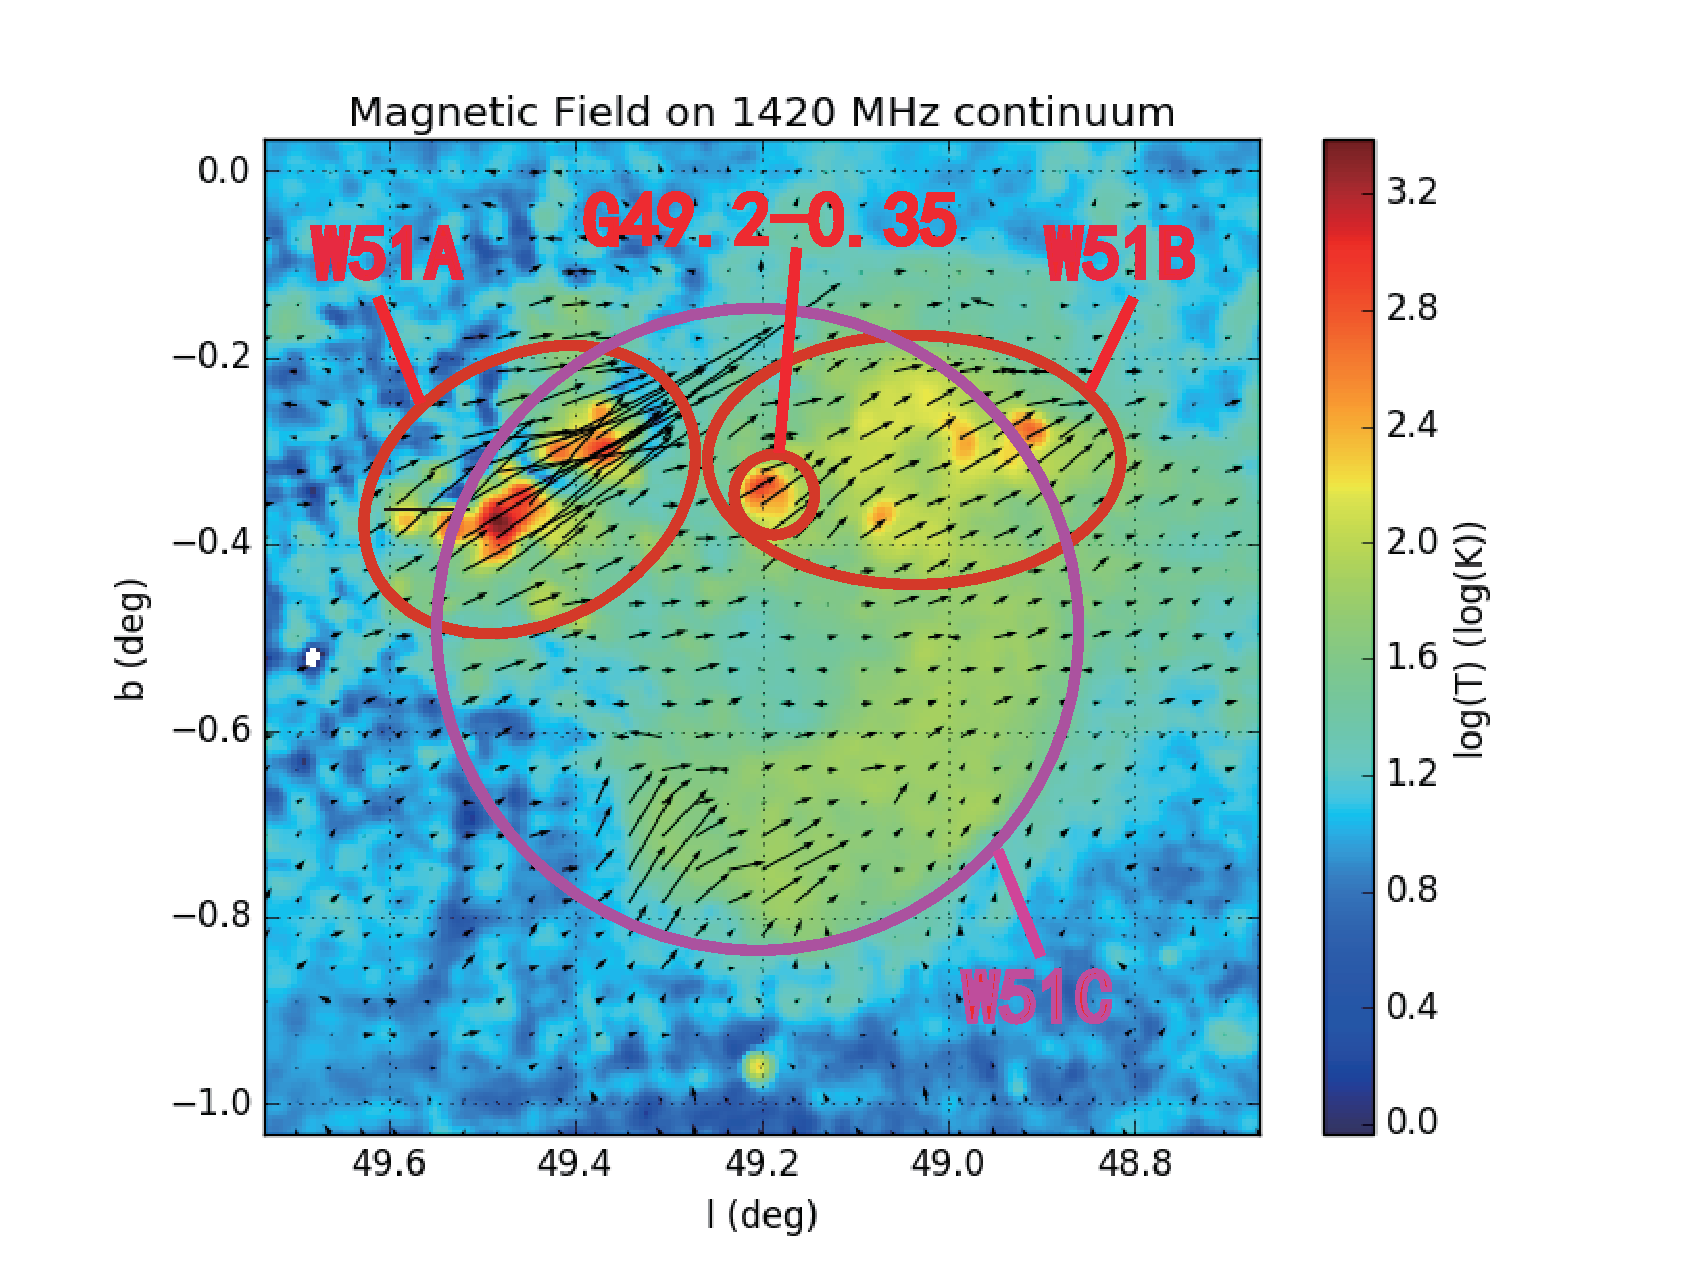
\includegraphics[width=0.495\textwidth]{mag0.eps}
   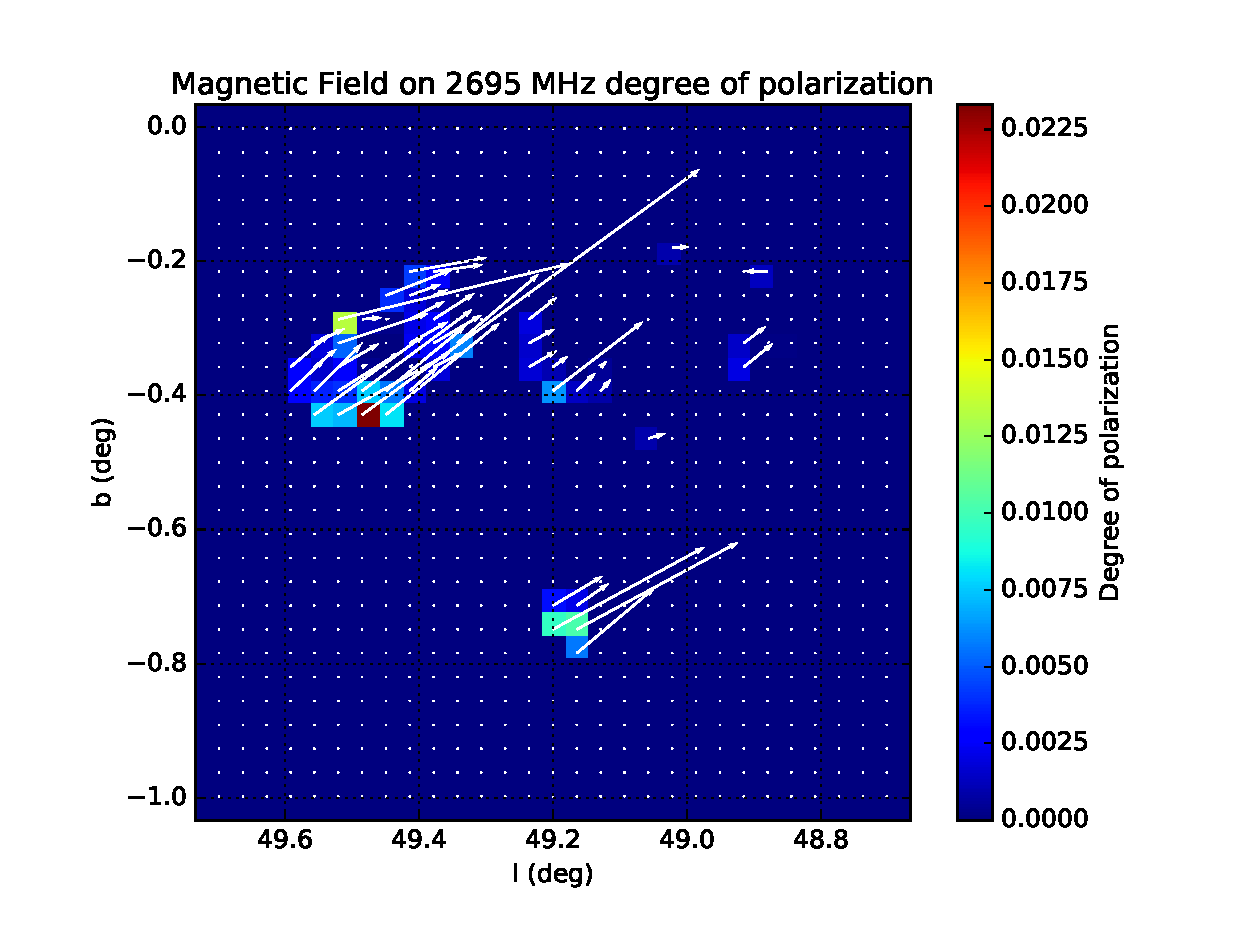
\includegraphics[width=0.495\textwidth]{modi_mag.eps}
   \caption{左图中彩色背景是来自VPGS的1.4 GHz连续谱图像。黑色的箭头代表没有扣仪器偏振的
   在2695 MHz的磁场方向,箭头长度代表偏振强度(mK),其中最大的强度是1581 mK。
   下图中,彩色背景是扣除仪器偏振后的2695 MHz的偏振度,白色箭头代表磁场方向,箭头长度代表
   偏振度,其中最大的偏振度是$2\%$。
   }
\label{fig:mag}
\end{figure*}

\section{模拟模型}
\label{W51Cmod}
这里我们使用三维磁流体模拟,忽略了粘滞度、电阻、热传导等耗散效应,引力和辐射冷却也不予考虑,
而具体的参数大多来源于前人的观测。
\citet{Sasaki2014}使用6 kpc作为距离估计SNR W51C前身星的质量超过20 M$_\odot$。
这个距离是一个上限,所以真实的质量可能更小。
在这个模拟中,我们取20 M$_\odot$为前身星质量,这样其爆发时抛射物的质量就是11 M$_\odot$
\citep{Sukhbold2016}。
\citet{Koo1995}也使用6 kpc为距离估计其爆发能量为3.6 $\times$ 10$^{51}$ ergs s$^{-1}$,
这个完全超出了典型的爆发能量,1 $\sim$ 3 $\times$ 10$^{51}$ ergs s$^{-1}$ \citep{Poznanski2013}。
根据\citet{Poznanski2013}的工作,对于W51C,爆发能量大约为1.0 $\times$ 10$^{51}$ ergs s$^{-1}$
是比较合理的。
虽然 \citet{Poznanski2013}只是估计了通过估计一些SNRs的动能得出这样的经验关系,可是他用的
遗迹都非常年轻,或者更合理的说是刚爆发的超新星,所以其动能几乎等于其总爆发能量。
而在我们的模拟中也是如此认为,即使如今观测到的遗迹热能与动能相当,我们认为爆发时总能量
几乎全部来自动能,爆发时的动能就是如今热能与动能的总和。
在对W51C的流体模拟中,我们认为对结果起作用的主要是动能,热能导致的辐射耗散影响不大。
实际上,W51C是一个中等年龄的遗迹,因此他的爆发能量应该是现如今动能和热能之和。
\citet{Koo1995}根据X-ray观测先推出热能,然后根据Sedov模型估算总的爆发能量\citep{1959sdmm.book.....S}。
采用最近测量的4.3 kpc的距离\citep{Tian2013},我们采取了与\citet{Koo1995}相同的方法
得到了1.3 $\times$ 10$^{51}$ ergs s$^{-1}$的爆发能量,这是一个相对来说更合理的结果。
当然,SNRs的爆发能量其实变化很大,所以这并不能作为一个决定性的证据说明哪个距离就是正确的。
4.3 kpc在目前看来只是更可靠一点,所以我们在模拟中取其为W51C的距离。
我们选择$48.89^{\circ}<l<49.51^{\circ}$, $-0.81^{\circ}<b<-0.19^{\circ}$这一区域
作为模拟研究的目标。
这样对于这个大约角直径有37\am的遗迹,其真实直径是46 pc。
如果采用\citet{Koo1995}推导的平均激波速度490\kms,其年龄为18000年。

我们通过一个用于模拟SNR解析演化的Python计算器\citep{Leahy2017a}估计得到介质平均密度为
0.21 cm$^{-3}$。
可是在我们的前期测试模拟中发现,均匀介质中演化的遗迹壳层会很薄,而W51C的壳层很厚。
此外,均匀介质分布其实是一种理想假设,实际情况中介质密度更多是随机分布。
为了模拟出介质的随机分布,我们采用了幂律的介质分布模型$N(\rho) = N_0 \rho^{-\alpha}$,
这里$N(\rho)$是像素数,表征了有某一个密度的格点的个数, $N_0$是一个常数,用来保证最终结果
满足平均密度估计,$\alpha$是一个幂律指数。
$\alpha$是正数,也就是说低密度的区域比高密度的区域更多更大。
举个粒子,在我们的模拟中,共有256 $\times$ 256 $\times$ 256个格点,那可能有一千万个点
密度低于0.21 cm$^{-3}$,而只有100个点密度高于21 cm$^{-3}$。
\citet{Parsons2012} 研究了SNR W51C周围的分子团块(包括致密团块),发现它们的质量分布
满足一个指数$\alpha$为2.4的幂律谱,这个结果暗含了真实的周围介质密度分布。
因为目前对这个区域没有原子氢密度分布的研究,所以我们取$\alpha=2.4$作为初始介质密度分布。
此外,为了模拟相互作用,我们在初始条件中加了一个密度为2 cm$^{-3}$直径为11 pc的分子云
(如图~\ref{fig:simulation}中间两幅图)。

\begin{figure*}
    \centering
    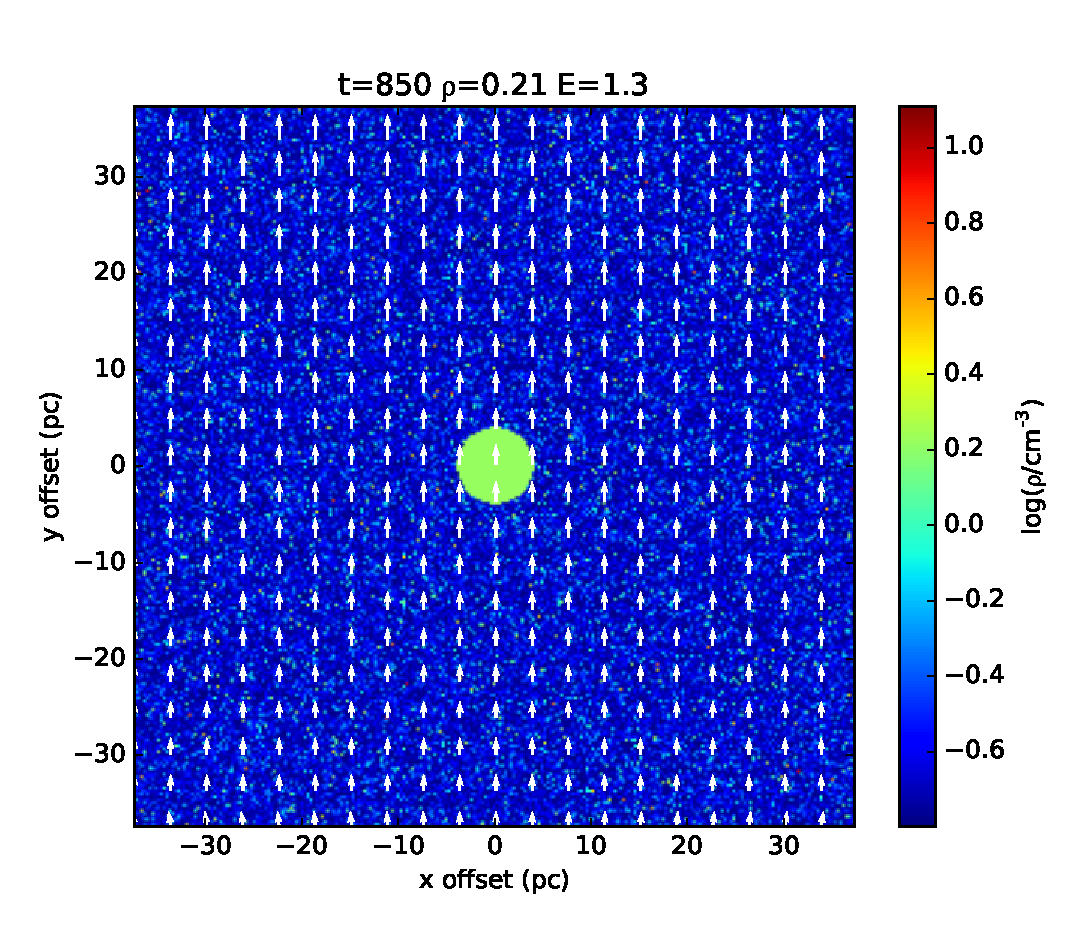
\includegraphics[width=0.323\textwidth]{rho850_density021_E13xy.eps}
    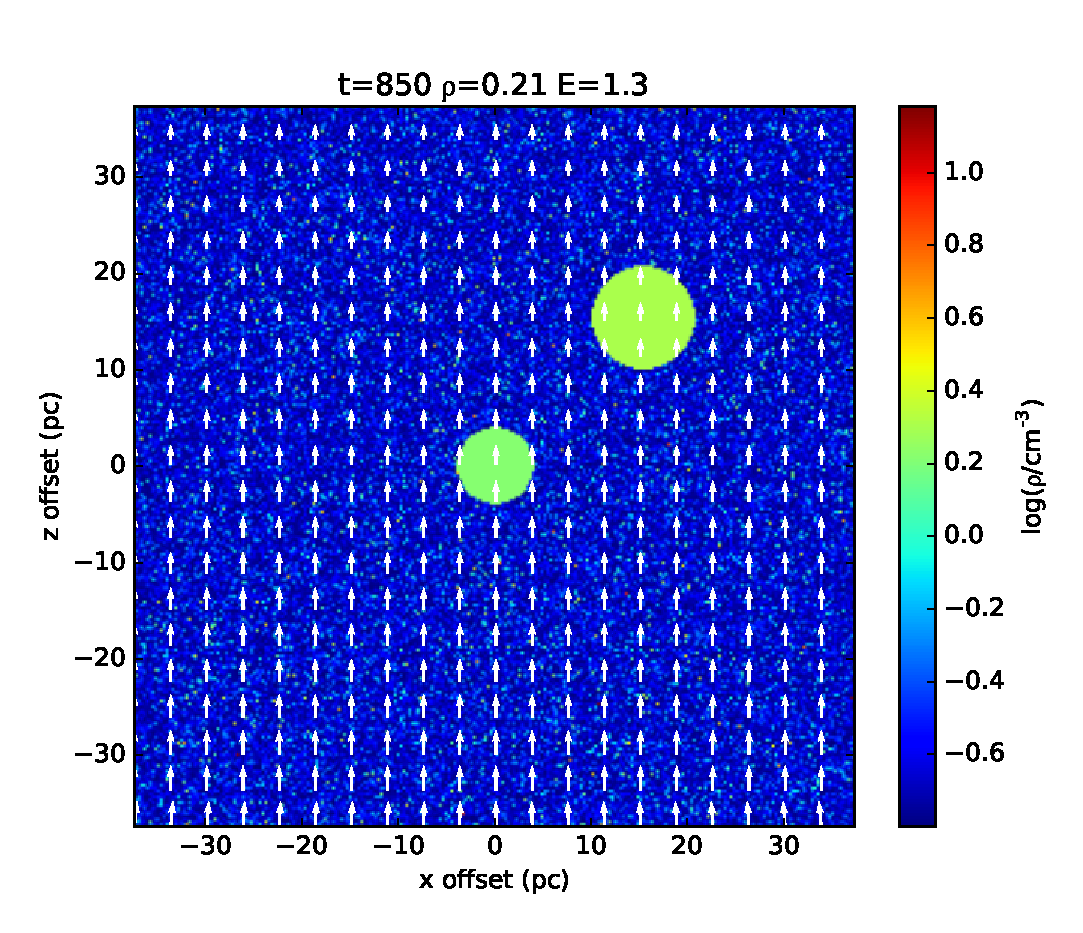
\includegraphics[width=0.323\textwidth]{rho850_density021_E13xz.eps}
    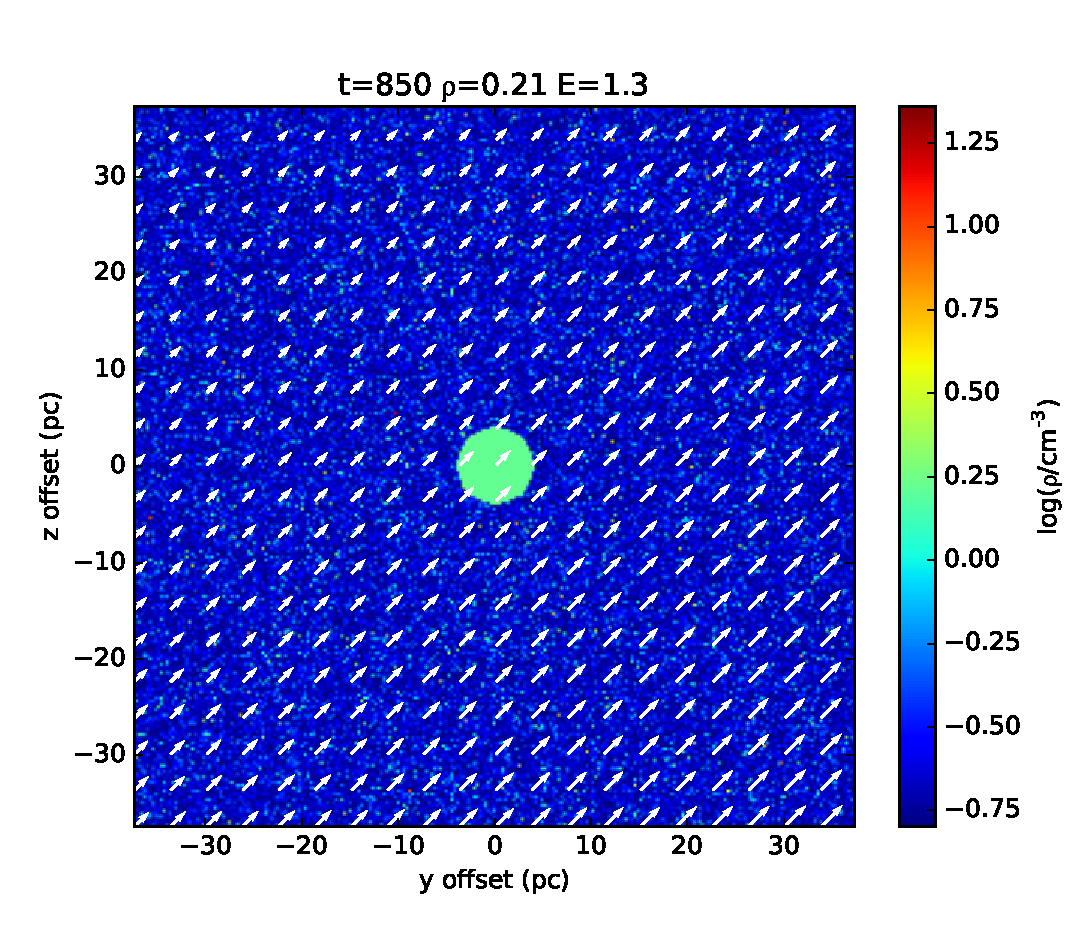
\includegraphics[width=0.323\textwidth]{rho850_density021_E13yz.eps}\newline
    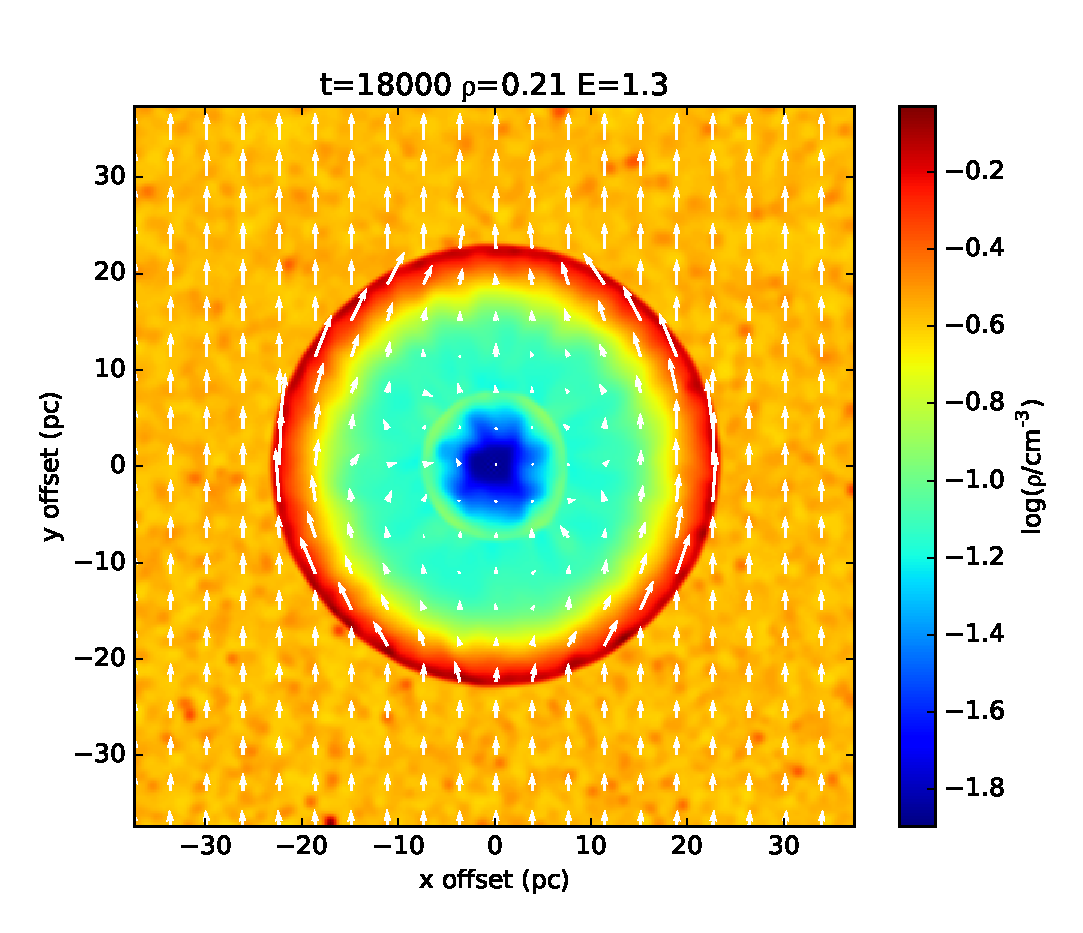
\includegraphics[width=0.323\textwidth]{rho18000_density021_E13xy.eps}
    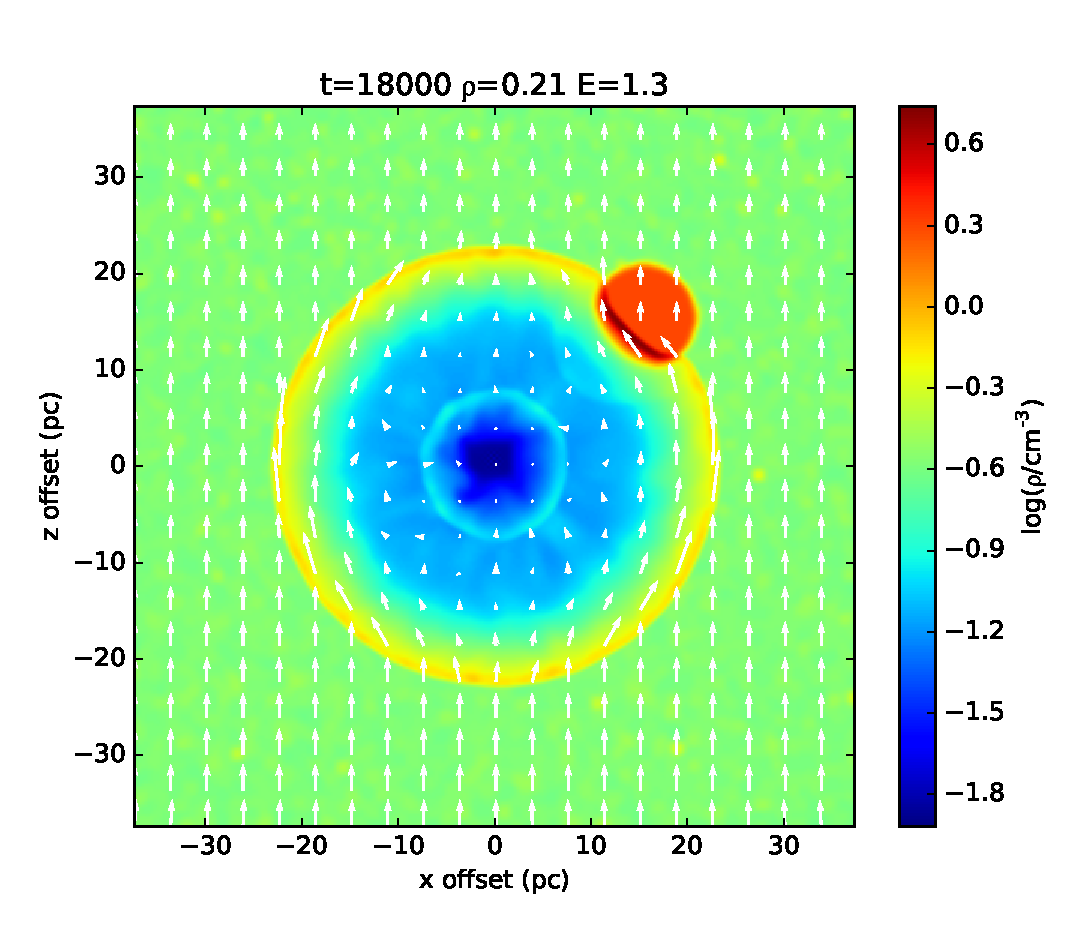
\includegraphics[width=0.323\textwidth]{rho18000_density021_E13xz.eps}
    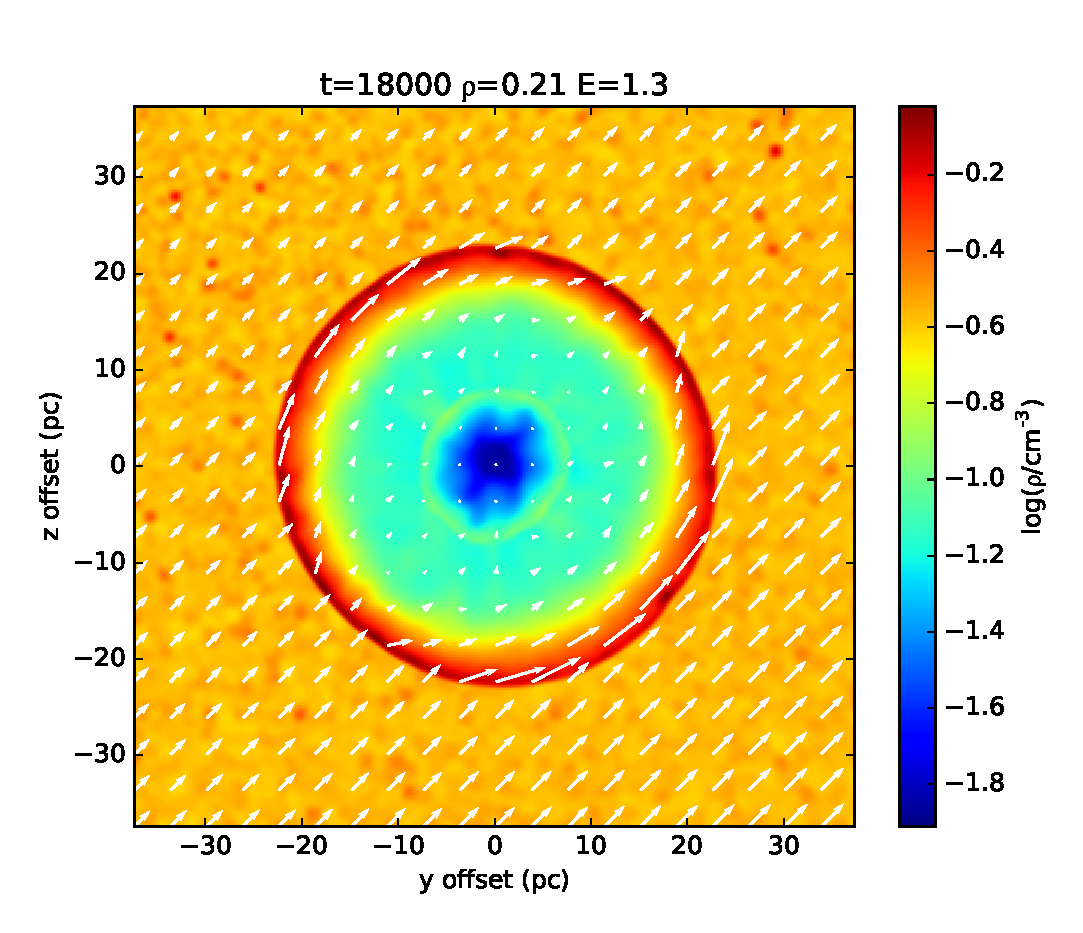
\includegraphics[width=0.323\textwidth]{rho18000_density021_E13yz.eps}
    \caption{模拟的密度-磁场图像。所有的图都是沿着一个三维立体图像沿着中心切片后得到的
    从不同方向看的结果。背景彩色图像是密度分布,白色箭头显示了磁场的方向和强度。上面三幅
    显示的是初始条件,下面三幅显示了经过18000年演化后的结果。上面三幅图中,中心磁场的强度
    是9$\mu G$。}
\label{fig:simulation}
\end{figure*}

因为W51C的壳层倾斜方向基本与银道面呈45$^{\circ}$夹角,所以我们在模拟中也设置了这样一个
角度。
我们在模拟中认为超新星爆发是球对称的,考虑到磁场,其遗迹的演化是柱对称的,所以为了产生一
个单边亮的壳层,我们需要设置不对称的初始介质分布,从而保证遗迹有一个边非常暗以至于其流量
低于射电望远镜观测灵敏度。
之前\citet{Orlando2007}通过设置密度或者磁场梯度以达到这一效果,
而在这一区域我们并没有观测到明显的密度梯度分布,所以在这个模拟中,我们通过设置较大的磁
场梯度来保证一边流量大,一边流量小到观测不到。
而银河系介质中平均磁场强度为4 $\mu$G到14 $\mu$G \citep{Haverkorn2015},我们模拟的尺度
为$75 \times \sqrt{2}$ pc。
所以,我们假设模拟中心磁场强度为9 $\mu$G,而磁场梯度为0.1 $\mu$G pc$^{-1}$。
磁场梯度如果再大,最小磁场或者最大磁场就会超过比较合理的范围。

我们模拟了大小为$1^\circ \times 1^\circ$的区域,对于4.3 pc的距离实际尺度75 pc $\times$
75 pc。
对于这个区域,我们使用256 $\times$ 256 $\times$ 256的网格来进行三维模拟,也就是说,
其分辨率是0.3 pc pixel$^{-1}$ (0.24\am pixel$^{-1}$)。
因为模拟时网格为立方体,为了得到近似为球对称的爆发,我们需要设置较大的初始爆发半径。
同时,早期的自由膨胀相的遗迹演化可以通过解析解得到,而超过自由膨胀相的演化就不太适合了,
所以初始爆发半径又不能太大以至于演化到绝热膨胀相。
所以,对于W51C,我们选取初始爆发半径为4 pc,对于这个遗迹,它需要花费850年达到这个
半径,而他的绝热膨胀相起始于3200年\citep{Leahy2017a},所以它达到初始半径时仍处于自由
膨胀相。
在图~\ref{fig:simulation}中,上面三幅图展示了模拟中采用的初始条件。

为了与真实的观测图像相比较,我们假设其射电辐射全部来自于同步辐射,并使用简化公式
$i(\nu)=C\rho B_{\perp}^{\beta + 1}\nu^{-\beta}$ \citep{Orlando2007}得到相对射电
流量体密度,这里$\nu$是辐射频率,C是一个常数,$\rho$是密度,$B_{\perp}$是垂直于视线方
向的磁场,$\beta$是同步辐射谱指数。
通过沿视线方向积分,$\int i(\nu) \mathrm{d}l$,我们可以获得可以与实际观测相比较的相对
射电流量密度。
在我们的三维模拟中,X轴被定义为视线方向。
对于相互作用区域,我们认为大约10$\%$的介质对射电流量密度有贡献,也就是说
$i(\nu)=0.1C\rho B_{\perp}^{\beta + 1}\nu^{-\beta}$。
$\nu$取1.4GHz,$\rho$和$B_{\perp}$是模拟过程中的主要变量,$\beta$对于W51C取0.25
\citep{1970AuJPA..14..133S}。
然后我们可以获得一个相对射电流量密度的图像,而要获得绝对射电流量密度需要得知常数C,这个
对于每个遗迹都不一样,因为其中包含了激波加速效率等变量,这些量对于每个遗迹都不一样,
要获得C需要将观测与模拟相对比得到。
但是相对射电流量已经能够告诉我们很多信息了。
用于比较的VGPS射电连续谱的分辨率是1\am,而模拟结果分辨率高很多,如果要将其与模拟结果比较
的话,需要将模拟结果分辨率平滑到与观测相近。
分辨率其实指的是观测源的半高全宽(the full width at half maximum, FWHM),对于用于平滑的
高斯方程:

\begin{equation}
  \begin{aligned}
    G(x)=\dfrac{1}{\sigma \sqrt{2\pi}}e^{-\dfrac{1}{2}(\dfrac{x-\mu}{\sigma})^2},
  \end{aligned}
\end{equation}

其FWHM定义为$2\sqrt{2ln2} \sigma$。
对于VGPS,其$\sigma$为0.42\am,我们模拟的分辨率是0.24\am pixel$^{-1}$,所以用于平滑
的$\sigma$为0.42\am/0.24\am pixel$^{-1}$=1.75 pixel,作为简化,我们取$\sigma$=2
pixel。

这个工作中我们模拟了SNR W51C演化18000年的结果,主要使用的参数都列在表~\ref{table:parameters}
中,其中没有参考文献的参数都来自于我们的估计。
当然,我们在模拟中也尝试过不同的参数,比如设置爆发能量为2.0和3.0 $\times$ 10$^{51}$ erg,
设置平均密度为0.13 cm$^{-3}$和0.3 cm$^{-3}$,设置谱指数为1.0和3.0。

\begin{table*}
  \caption{用于W51C模拟的参数}
  \label{table:parameters}
  \centering
  \begin{tabular}{l l l}
      \hline\hline
      参数                         & 值              & 参考文献               \\
      \hline
      抛射质量                      & 11 M$_{\odot}$ & 1, 2\\
      初始爆发动能                  & 1.3$\times$ 10$^{51}$ ergs & 3, 4\\
      模拟初始半径                  & 4 pc            &\\
      模拟起始时间                  & 850 years       & 5\\
      \hline
      平均密度                      & 0.21\ cm$^{-3}$ & 4, 5\\
      密度分布指数 ($\alpha$)       & 2.4             & 6\\
      磁场梯度                      & 0.1 $\mu$G pc$^{-1}$    &\\
      中心磁场强度                  & 9 $\mu$G        &\\
      平均原子质量                  & 1.3             &\\
      绝热系数                      & 5/3             &\\
      温度                         & 100 K           &\\
      \hline
      同步辐射谱指数 ($\beta$)       & 0.25            & 7\\
      距离                          & 4.3 kpc         & 8\\
      \hline
  \end{tabular}\\
  \tablerefs{(1)\citealt{Sasaki2014}; (2)\citealt{Sukhbold2016}; (3)\citealt{Poznanski2013}; (4)\citealt{Koo1995};
  (5)\citealt{Leahy2017a}; (6)\citealt{Parsons2012}; (7)\citealt{1970AuJPA..14..133S}; (8)\citealt{Tian2013}}
\end{table*}




\section{观测分析及模拟结果}
\label{W51Cres}

图~\ref{fig:mag}是W51C实际观测到的磁场结构。
我们能看到其中有四个区域有很强的偏振:东北(NE)、中部(M)、西北(NW)、南部(S)。
这四个区域的磁场方向相近,只有东北的方向有点小混乱,同时东北区的偏振是最强的。
去除仪器偏振之后,西北区域的偏振基本不见了,而其它三个区域的偏振仍然存在,这三个区域东北
、中部、南部分别对应实际的三个源W51A、G49.2-0.35、W51C。
此外,去除仪器偏振后,东北区的偏振变得规则了,这可能意味着我们已经去除了足够的仪器偏振。


\begin{figure*}
    \centering
    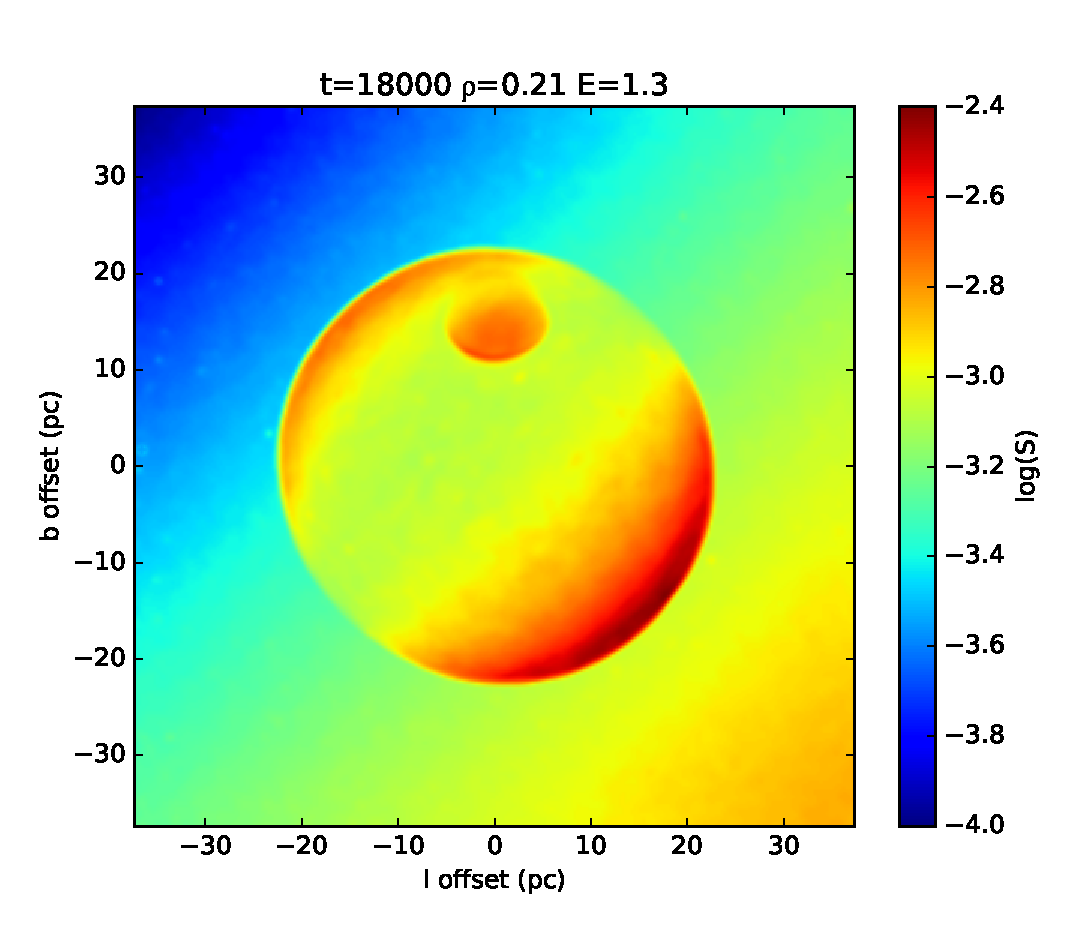
\includegraphics[width=0.472\textwidth]{t18000_density021_E13_s0.eps}
    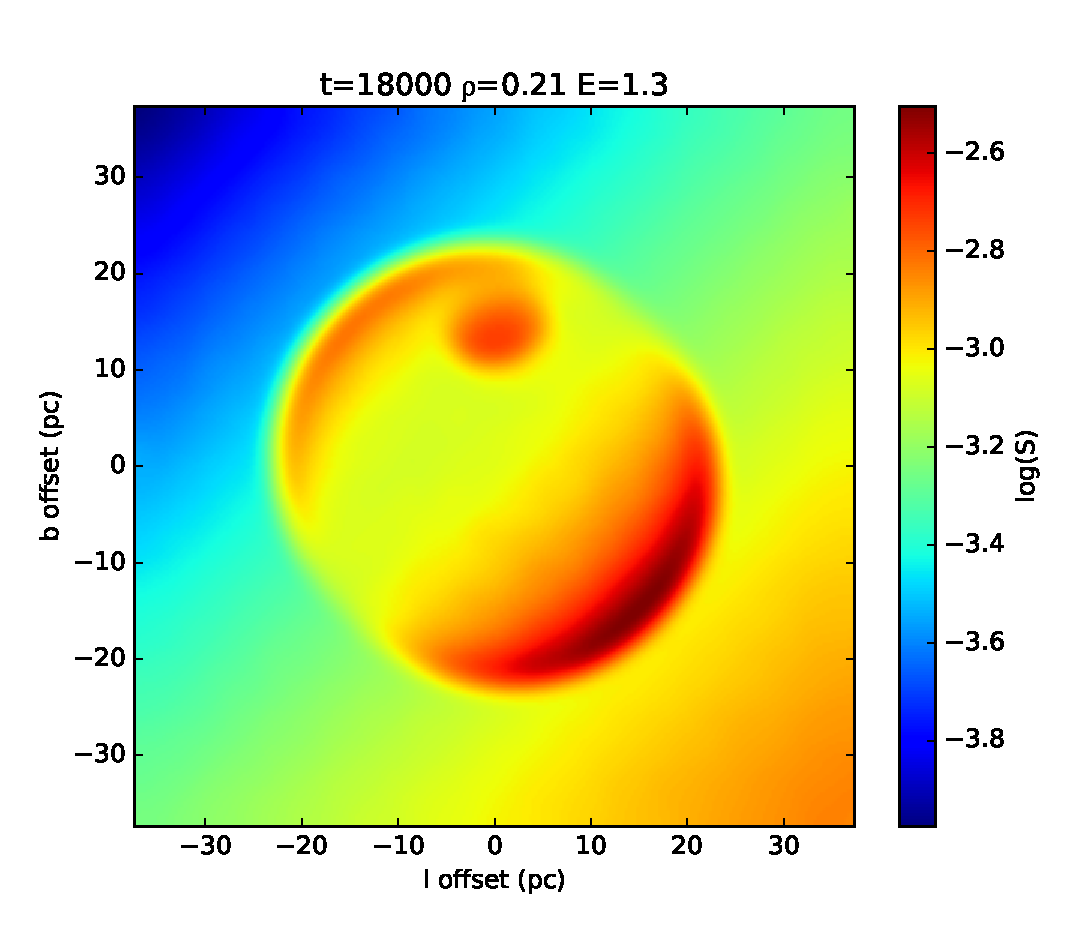
\includegraphics[width=0.472\textwidth]{t18000_density021_E13_s4.eps}
    \caption{SNR W51C演化18000年后的相对射电流量密度。右侧图像是$\sigma$=2的高斯平滑结果。
    这里设定距离为4.3 kpc,所以1 pc对应着0.8\am。}
\label{fig:flux}
\end{figure*}

主要的模拟结果在图~\ref{fig:simulation}中,我们能看到两侧激波区和相互作用区域有明显的
磁场放大。
在y-z平面中,左上角和右下角壳层的磁场强度大于他们的周围区域,右下角的磁场大于左上角的。
遗迹内部的密度和磁场强度都变得很低,外部壳层很致密,并有很强的磁场。
此外,遗迹内部有一层磁场密度比外壳层低,但是明显比周围要高一些的薄薄的壳层。

\begin{figure*}
    \centering
    \includegraphics[width=0.472\textwidth]{change.eps}
    \caption{这是图~\ref{fig:flux}的右图中左上到右下的流量切线图。 }
\label{fig:change}
\end{figure*}

图~\ref{fig:flux}是从密度图转化而来的相对射电流量密度图,用的谱指数是2.4。
我们也测试过谱指数为1.0和3.0的模拟。
谱指数为1.0时,射电图像呈现更过随机成分,但是别的特征与使用2.4时相似。
谱指数为3.0时,射电图像与使用2.4时并无太大差别。
因此,我们只在这里展示使用谱指数为2.4的图像。
左侧是直接转化的图像,右侧是使用$\sigma$=2高斯平滑后的图像。
可见左上角的壳层弱了很多,但明显还是有一定辐射。
图~\ref{fig:change}是图~\ref{fig:flux}中右图沿着左上到右下的流量密度变化,这显示出
左上角辐射流量密度大约是右下角的一半,而其实我们期待它应该更少。
遗迹区域中心流量是最低的,此外相互作用区也有明显的辐射。
图~\ref{fig:moreflux}展示了不同参数下的模拟结果。

\begin{figure*}
    \centering
    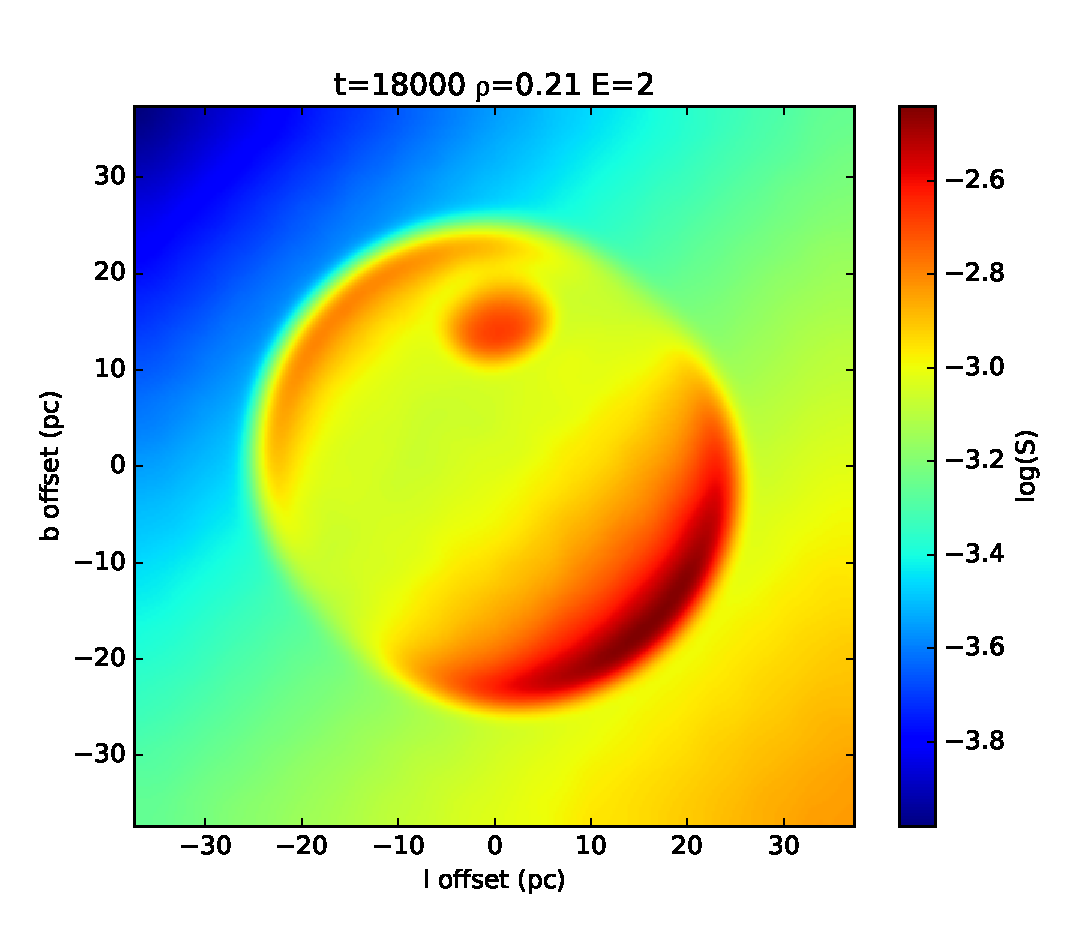
\includegraphics[width=0.472\textwidth]{t18000_density021_E2.eps}
    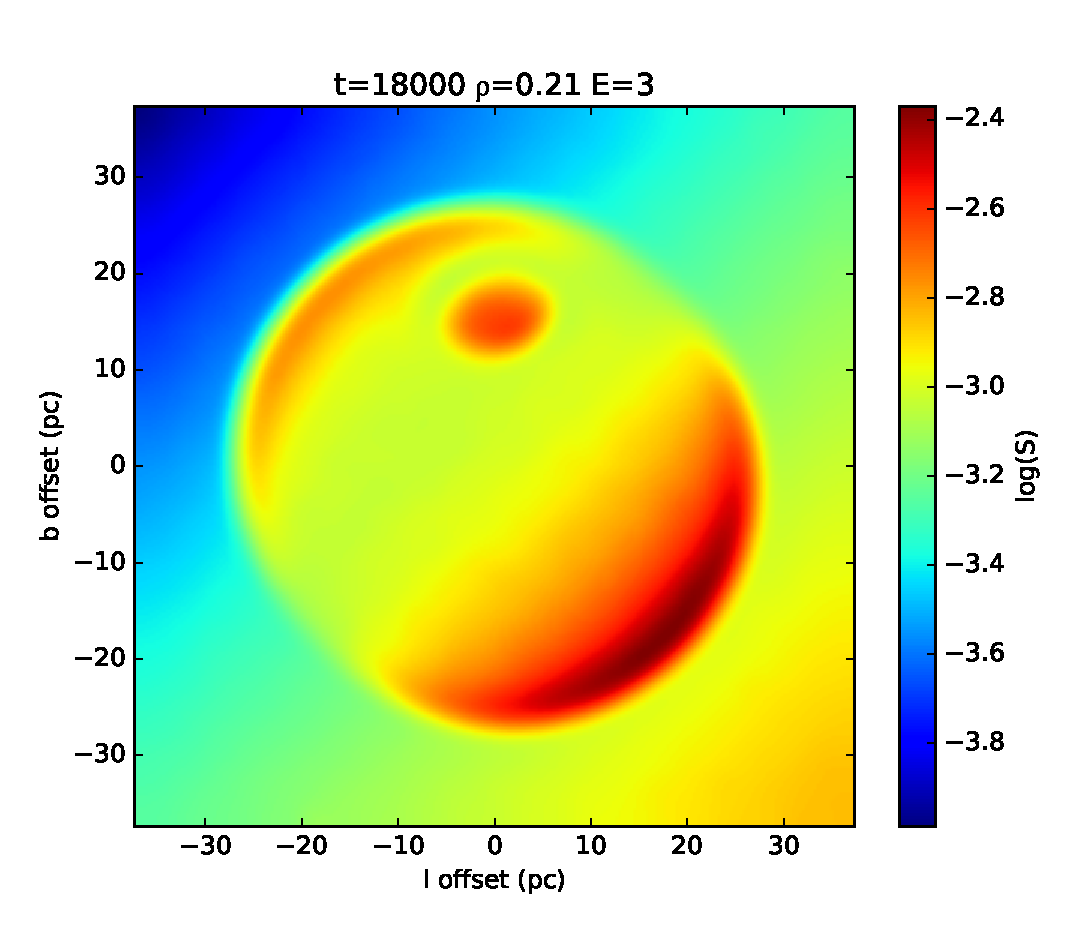
\includegraphics[width=0.472\textwidth]{t18000_density021_E3.eps}\newline
    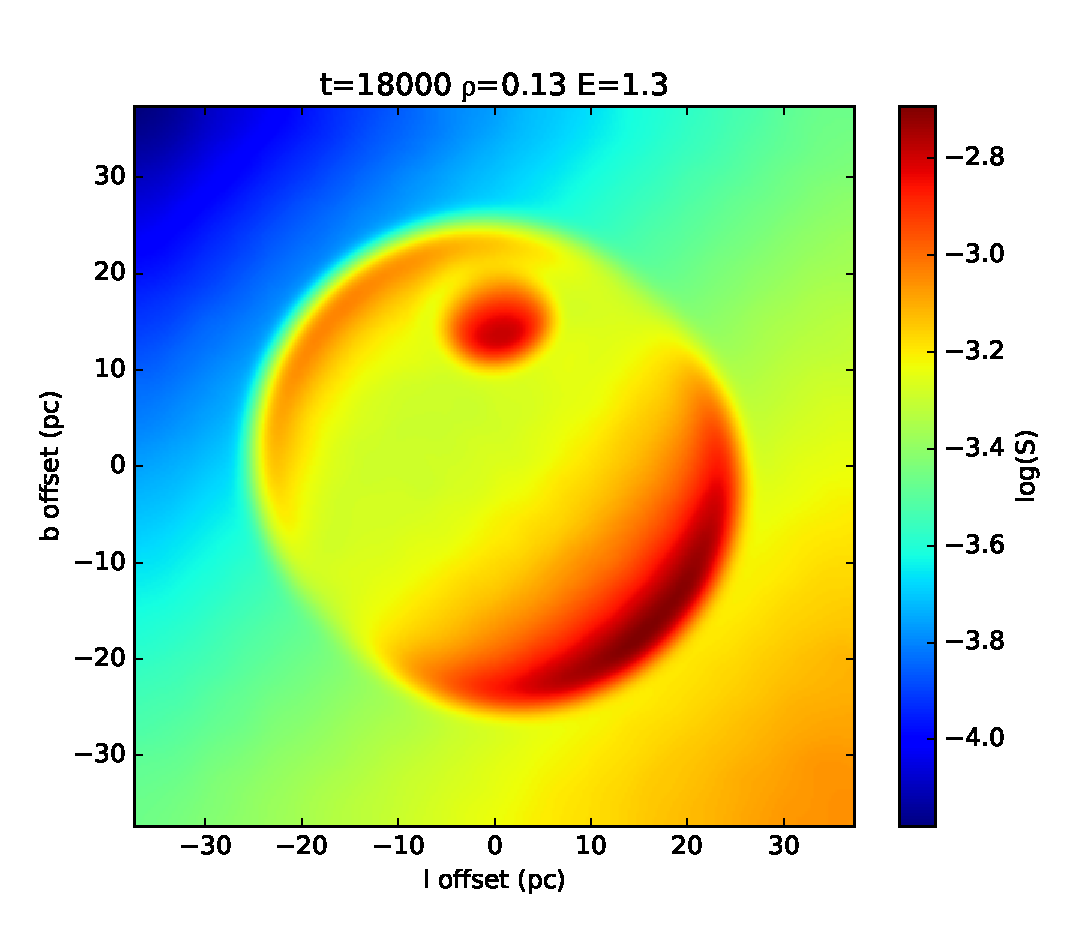
\includegraphics[width=0.472\textwidth]{t18000_density013_E13.eps}
    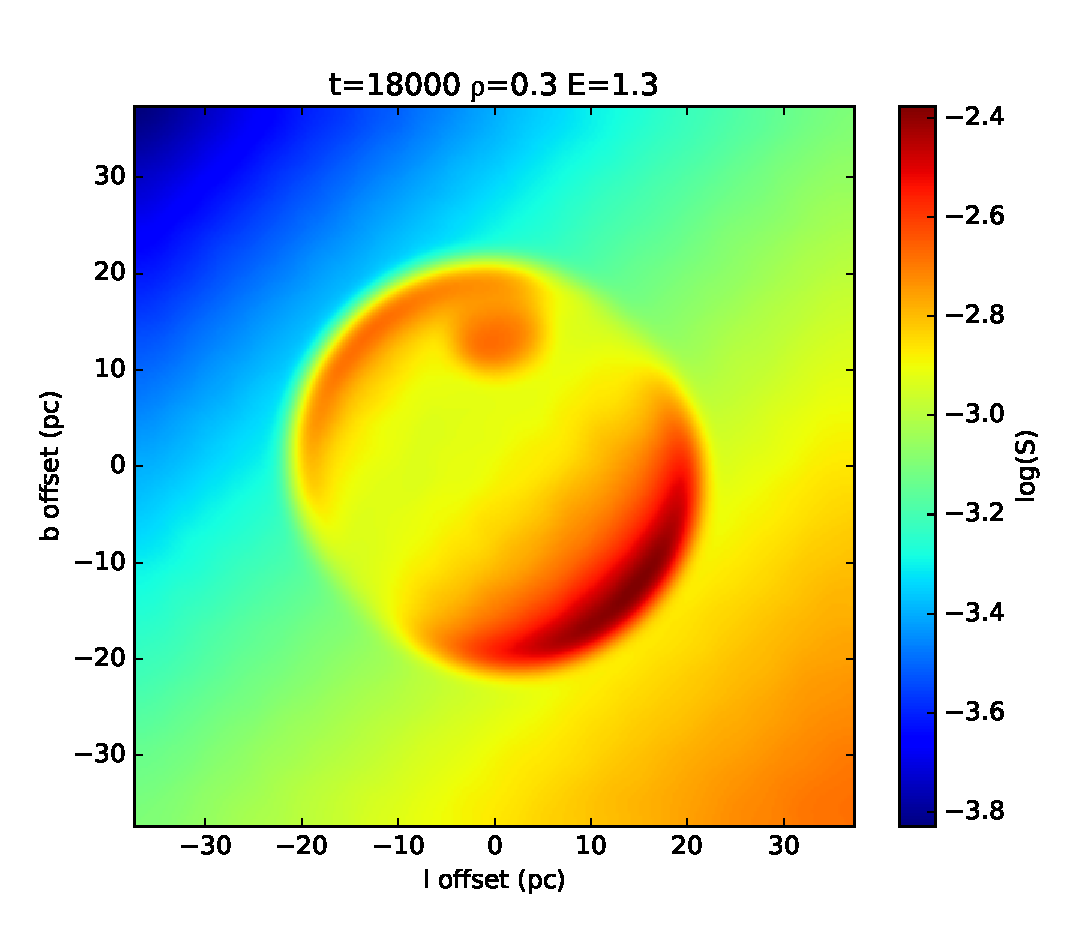
\includegraphics[width=0.472\textwidth]{t18000_density03_E13.eps}
    \caption{这是$\sigma$=2时不同参数下的相对射电流量密度图。 顶部两幅图为将初始爆发动能改为
    2.0和3.0 $\times$ 10$^{51}$ ergs的结果, 下面两幅图为将平均介质密度改为
    0.13 cm$^{-3}$和0.3 cm$^{-3}$的结果。}
\label{fig:moreflux}
\end{figure*}

之前,对这个区域已经有高分辨率的1720 MHz的观测\citep{2005ASPC..340..334B},但是还没
有与之对应的高分辨率的1665/1612 MHz观测。
这几个频率是羟基分子(OH)在射电波段的主要跃迁频率,对于我们研究超新星遗迹与分子云相互作用
有重要研究价值。
而THOR数据极高的分辨率提供给我们绝佳的机会来揭示1720 MHz辐射与 1720/1665/1612 MHz吸收的
空间位置关系。
图~\ref{fig:OH}是这个区域羟基OH的谱线图,彩色背景是THOR 1.4 GHz的连续谱图像,白色的
谱线为每个黑色方格中的平均结果。
当然,这里我们要说明,我们模拟中的相互作用区域的射电辐射与这个小电离氢区G49.2-0.35的射电
辐射不是一件事,实际观测到的射电辐射可能是电离氢区与相互作用区域在视线方向重合后相互叠加
的效果。
事实上,我们并没有直接探测到相互作用区域的射电辐射,但是1720 MHz OH脉泽和微弱但确实存在
的射电偏振辐射让我们认为它确实存在。
G49.2-0.35中射电亮的区域也呈现出明显的1720/1665/1612 MHz OH吸收线,然而射电暗的区域却
呈现出较宽的发射线而且1665 MHz OH 辐射非常强。
同时,有一些发射和吸收特征明显远离这个小电离氢区,所以应该是与周围前景或背景有关,这让我
们猜测G49.2-0.35的前景或背景会一定程度上影响我们看到的G49.2-0.35区域的谱线。
不过,虽然谱线来源或许不同,但是其特征速度都相似,因此应该都来源于W51复合体。

\begin{figure*}
   \centering
   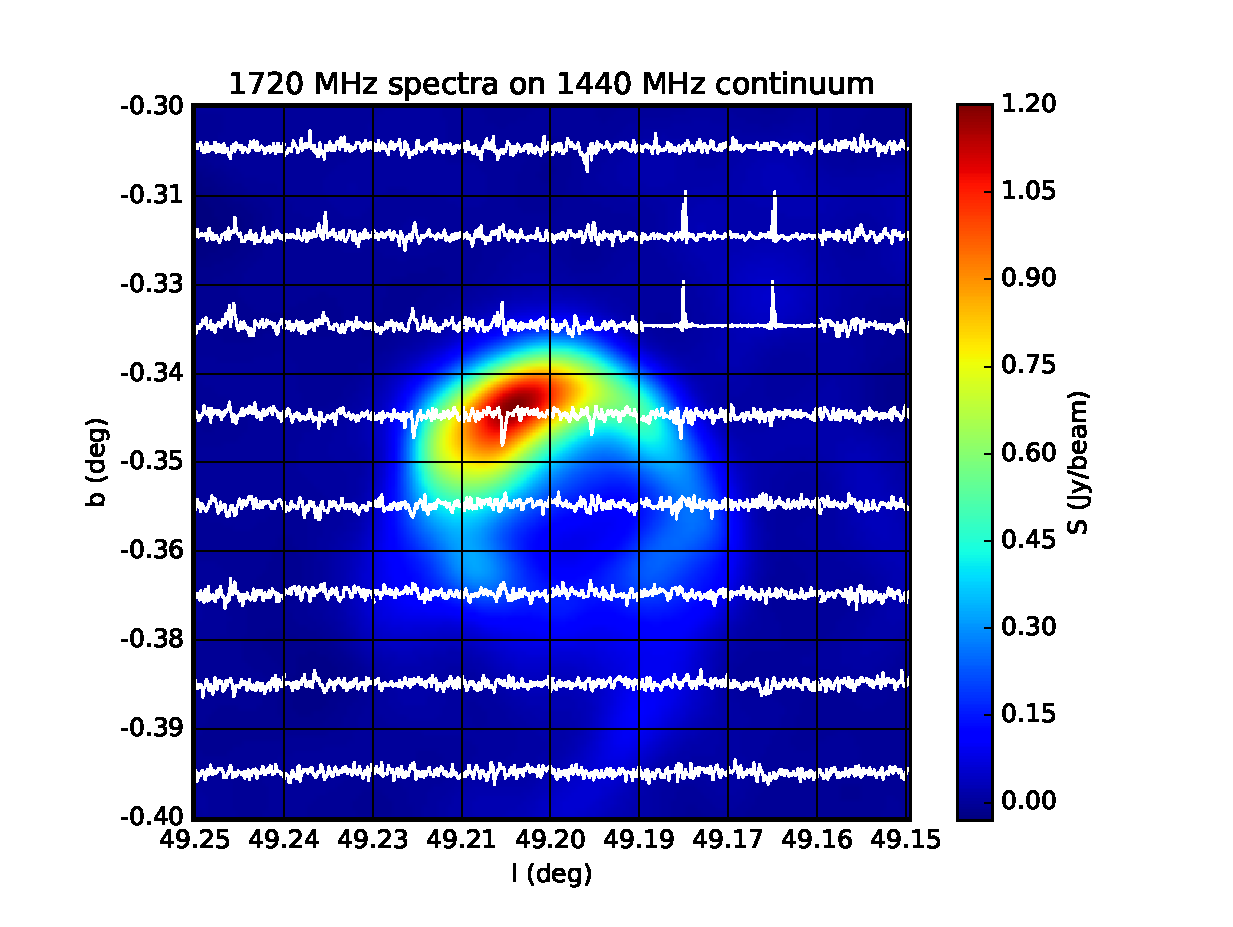
\includegraphics[width=0.472\textwidth]{s_1720.eps}
   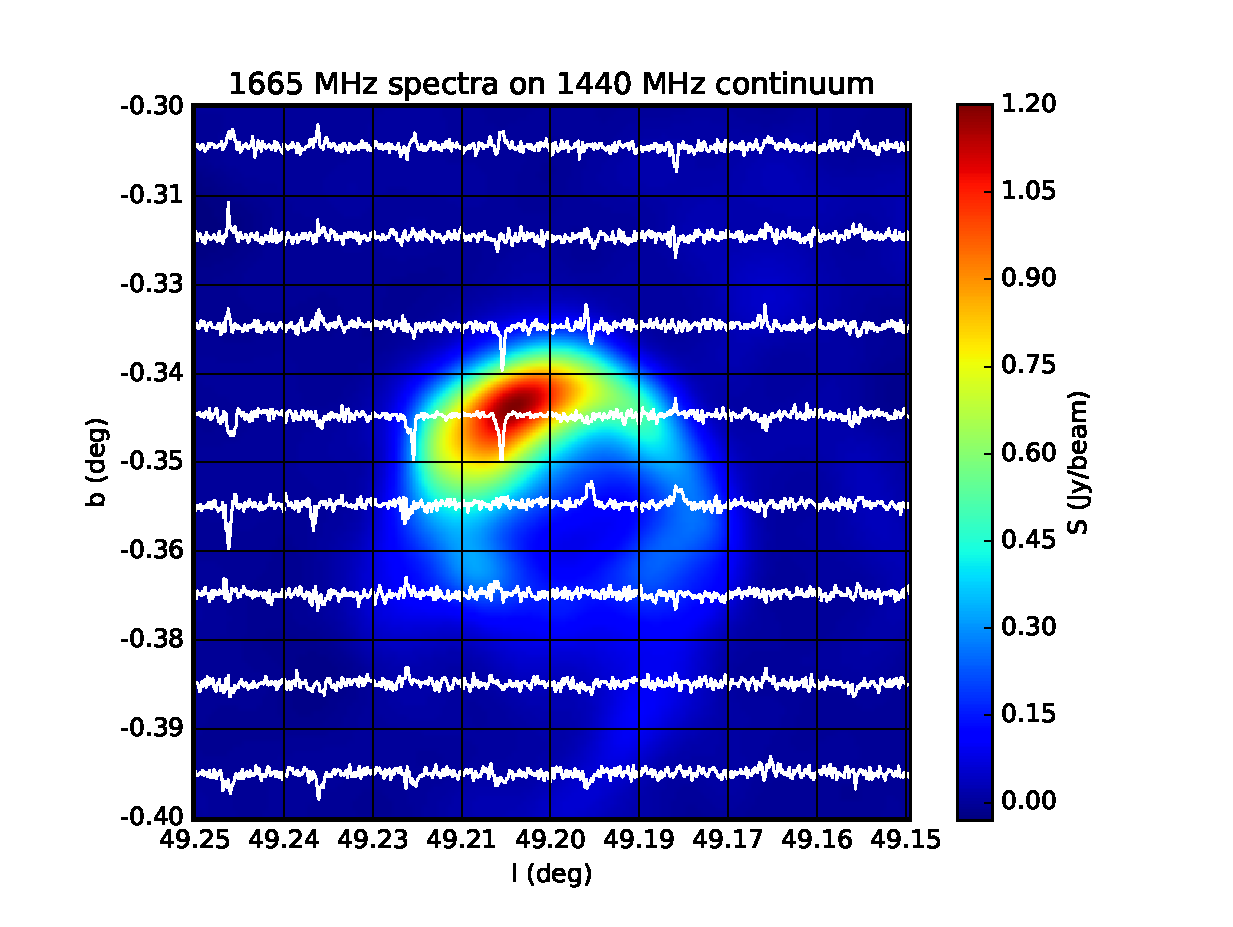
\includegraphics[width=0.472\textwidth]{s_1665.eps}
   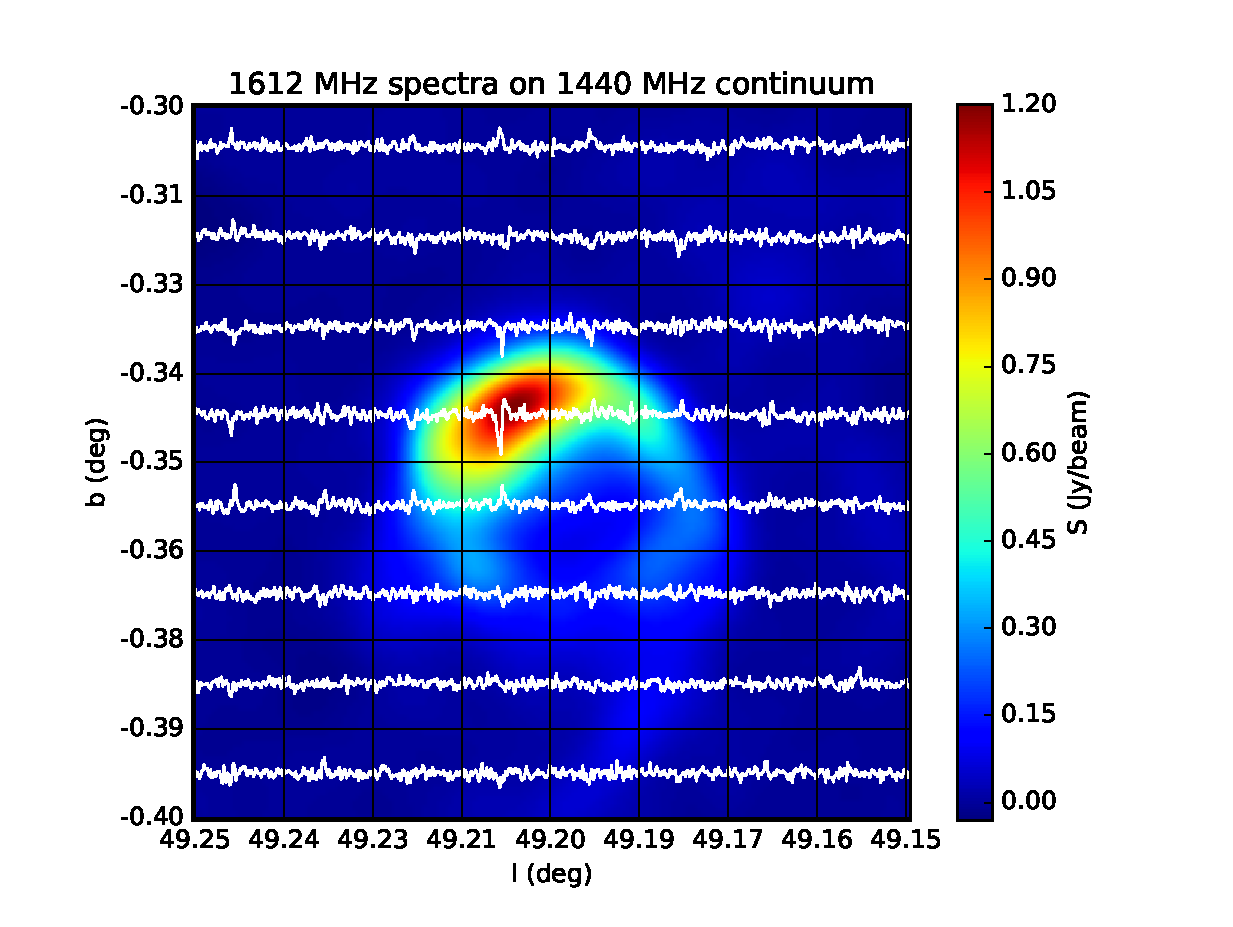
\includegraphics[width=0.472\textwidth]{s_1612.eps}
   \caption{三幅图分别展示了G49.2-0.35区域三个频率(1720/1665/1612 MHz)的OH谱线图。
   彩色背景是THOR数据的1440 MHz连续谱图像。谱线是每一个黑色方格区域中中-58.5\kms到
   135 \kms的平均谱线。第一幅图中,区域$49.16^{\circ}<l<49.19^{\circ}$,
   $-0.34^{\circ}<b<-0.31^{\circ}$中的标度与其它区域不同,因为这个区域里的1720 MHz OH
   脉泽非常强,如果使用相同标度其谱线就超出整个图形了,所以这个区域的谱线强度是除了20的。}
\label{fig:OH}
\end{figure*}

图~\ref{fig:spectra}展示了G49.2-0.35和1720 MHz OH脉泽的相对位置和谱线。
其中,1720 MHz OH脉泽非常强,而且明显距W51B中的小电离氢区G49.2-0.35一定距离,这在之前
的观测中因为分辨率的原因未被看到过。
1720 MHz OH脉泽有两个峰值,而1720 MHz OH的吸收峰值与脉泽峰值有大约2 $\sim$ 3 \kms的偏离。
有趣的是,吸收谱中,观测频率越大,吸收峰值速度也越大,这可能是一个帮助我们研究相互作用区域与
这个电离氢区相互位置的重要线索。

\begin{figure}
   \centering
   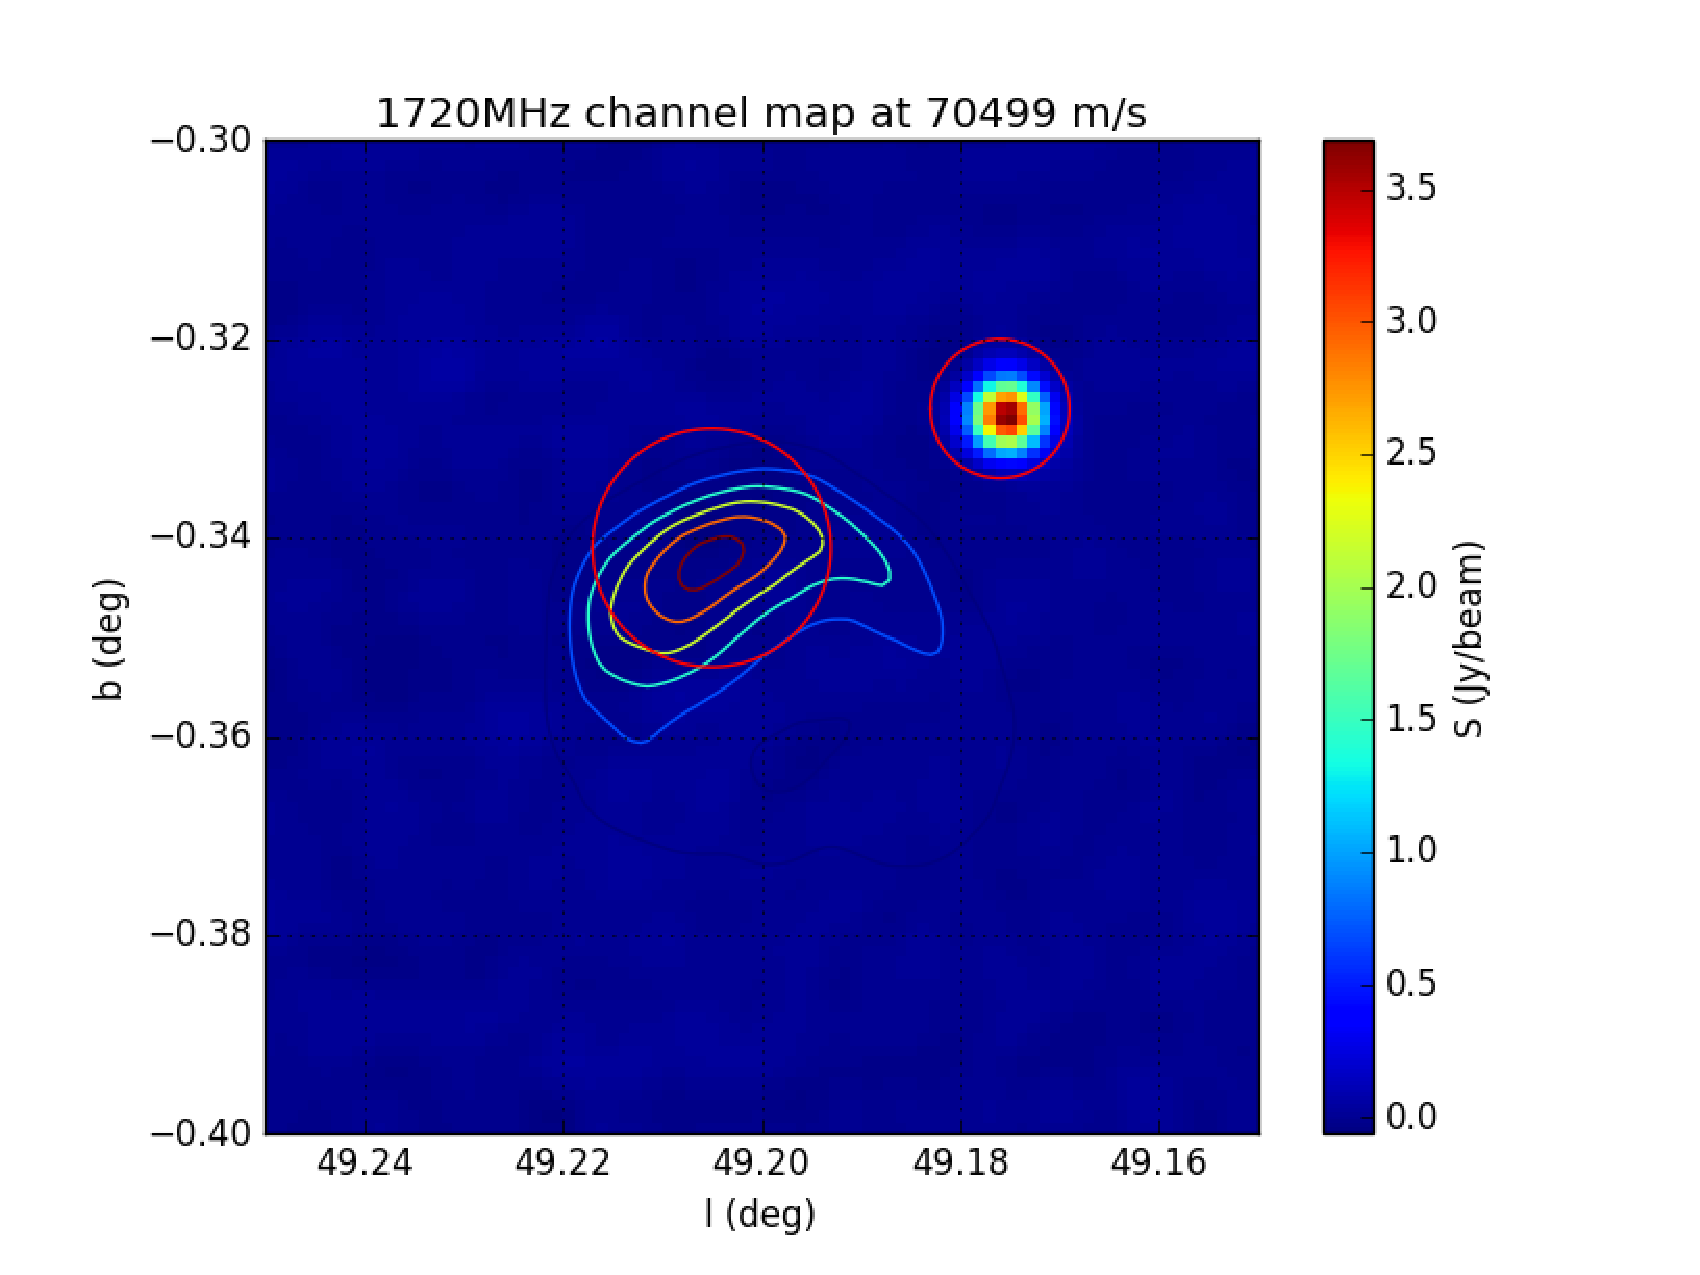
\includegraphics[width=0.472\textwidth]{contour.eps}
   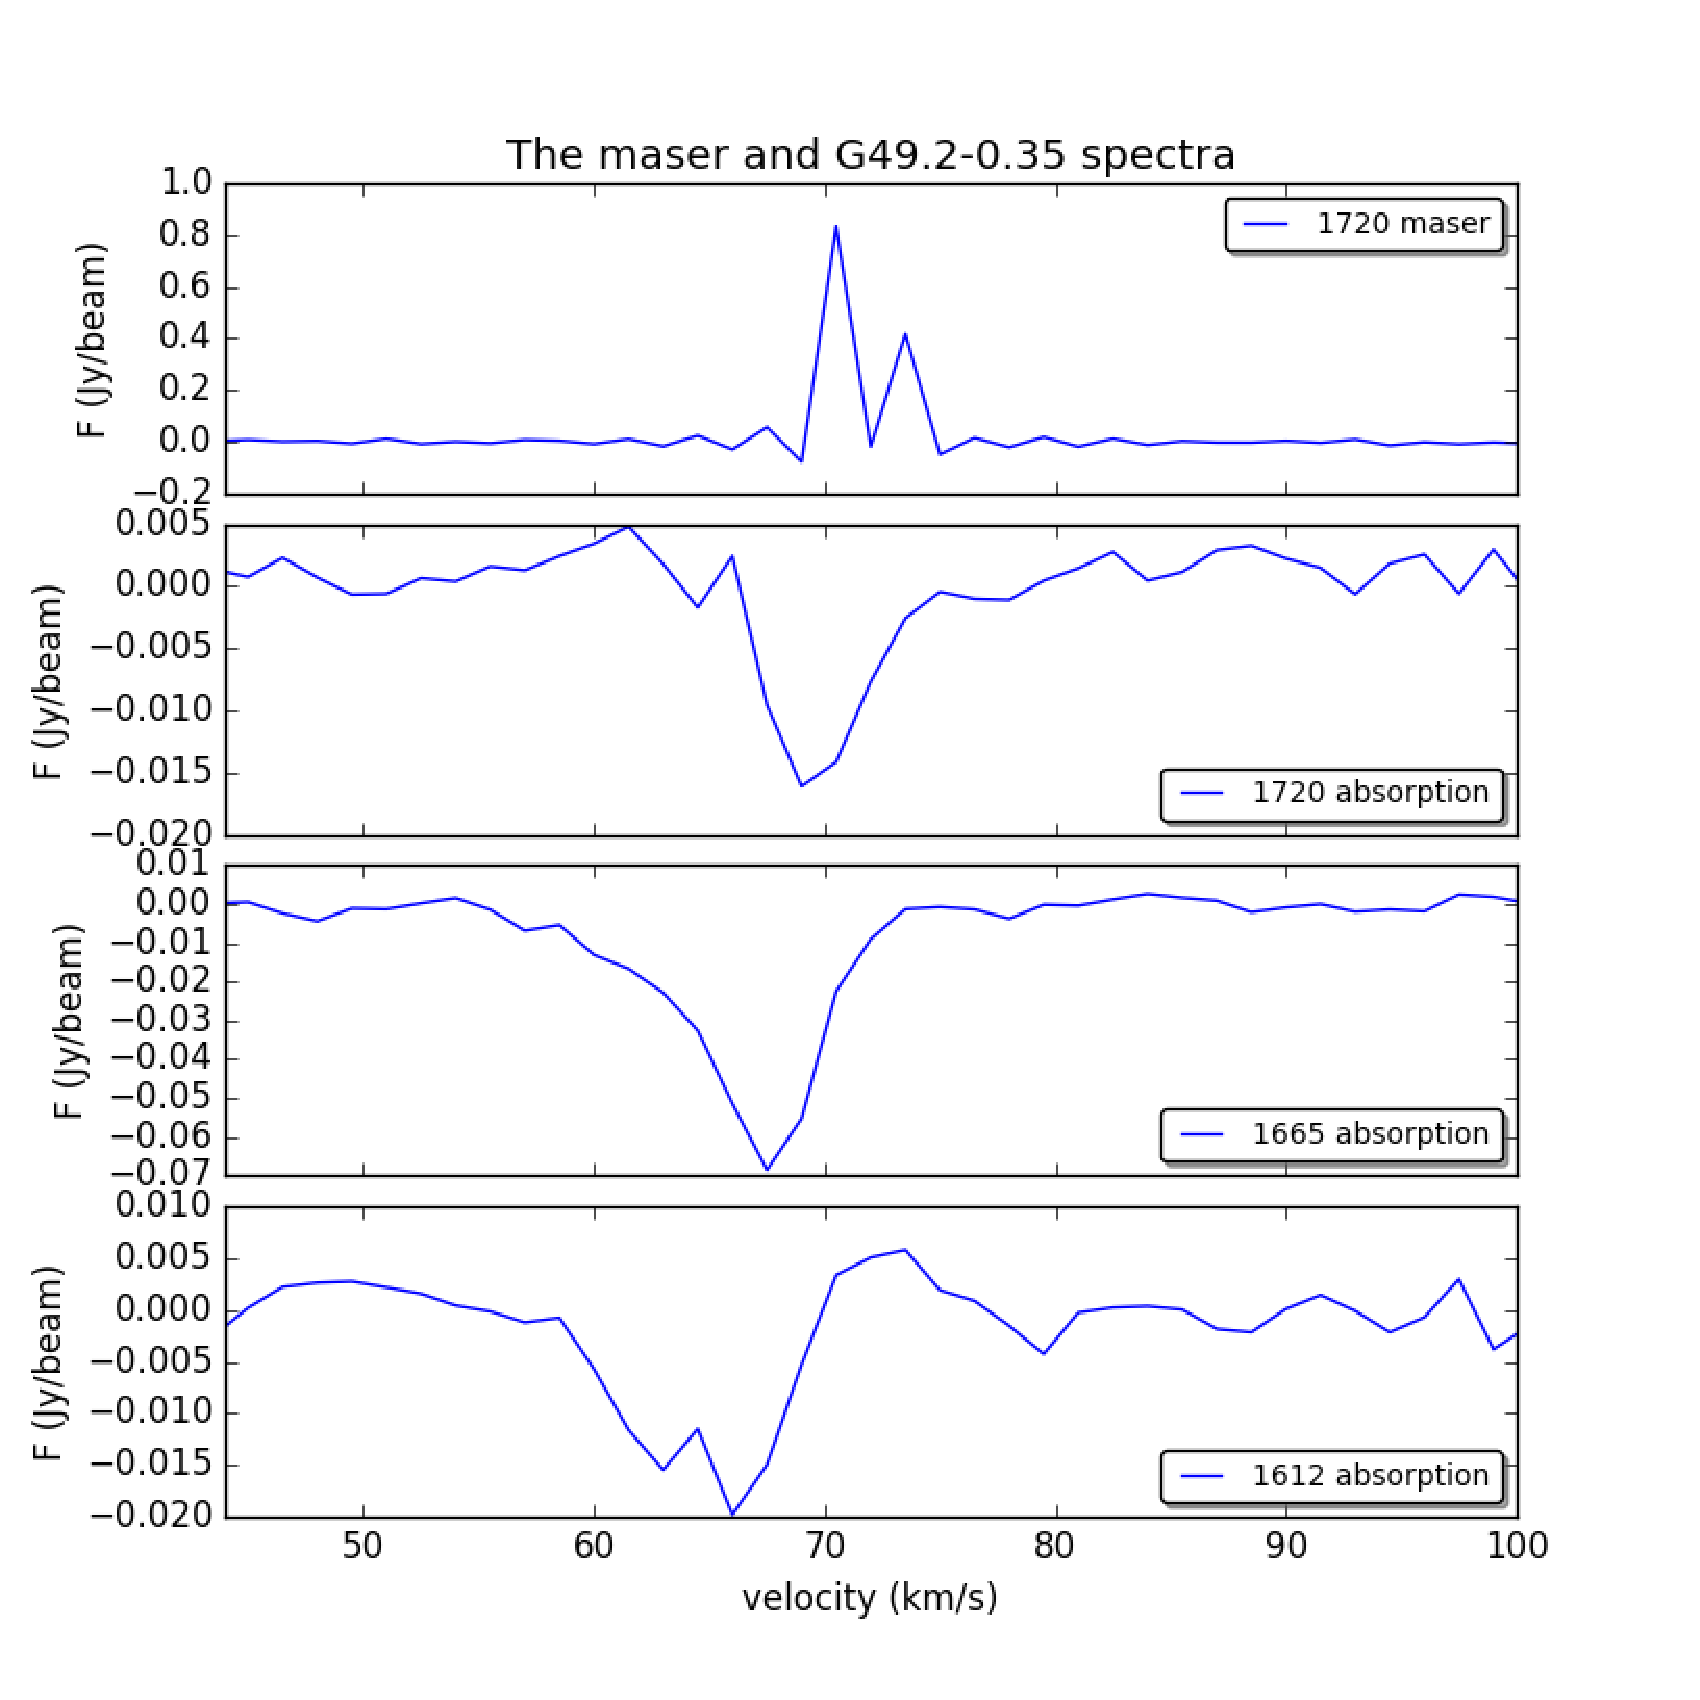
\includegraphics[width=0.472\textwidth]{spectra.eps}
   \caption{左侧的图中,彩色背景是G49.2-0.35区域的1720 MHz谱线在70.5 \kms的通道图,
   彩色等高线对应的是THOR的1440 MHz连续谱,右边的红色圆圈是我们提取脉泽发射线的区域,
   左边的红色圆圈是我们提取吸收谱的区域。右侧图是这两个区域的谱线,最上面一个是1720 MHz
   OH脉泽发射线的谱,下面的三个是不同频率处的吸收谱。}
  \label{fig:spectra}
\end{figure}

\section{讨论}
\label{W51Cdis}
\subsection{新的东北部的壳层}
为了模拟出单壳层的遗迹,我们参考了\citet{Orlando2007}的方法,然后发现壳层的厚度与星际
介质的密度分布有关。
在均匀介质中,壳层通常更薄,为了模拟出W51C的厚度,我们选择了幂律分布的介质密度作为模拟
中介质分布的初始条件。
无论怎么调整参数,我们的模拟总是显示与电离氢区W51A重合的区域有一个新的壳层。
因为W51A非常亮,可能它完全覆盖了新的壳层,而之前的研究一直没有认识到这一点(见
图~\ref{fig:compare}中的比较)。

\begin{figure*}
   \centering
   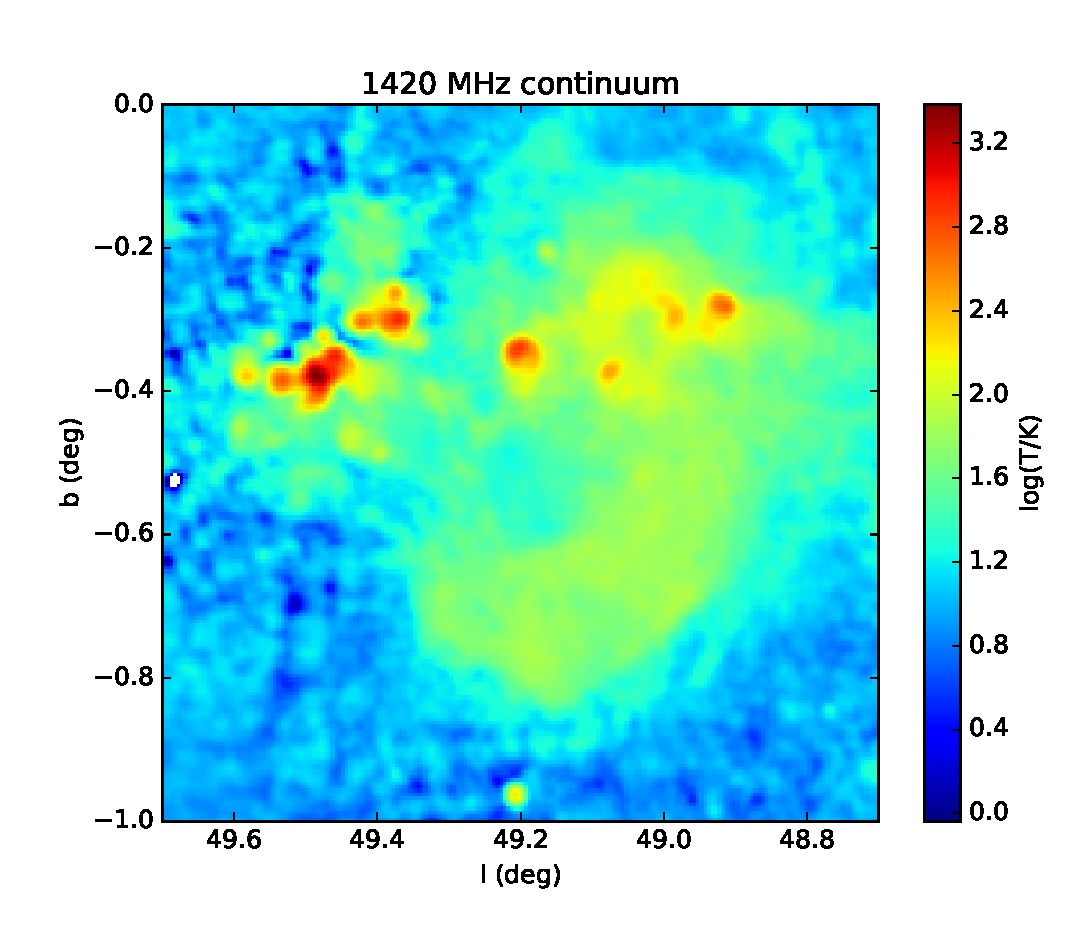
\includegraphics[width=0.472\textwidth]{continuum.eps}
   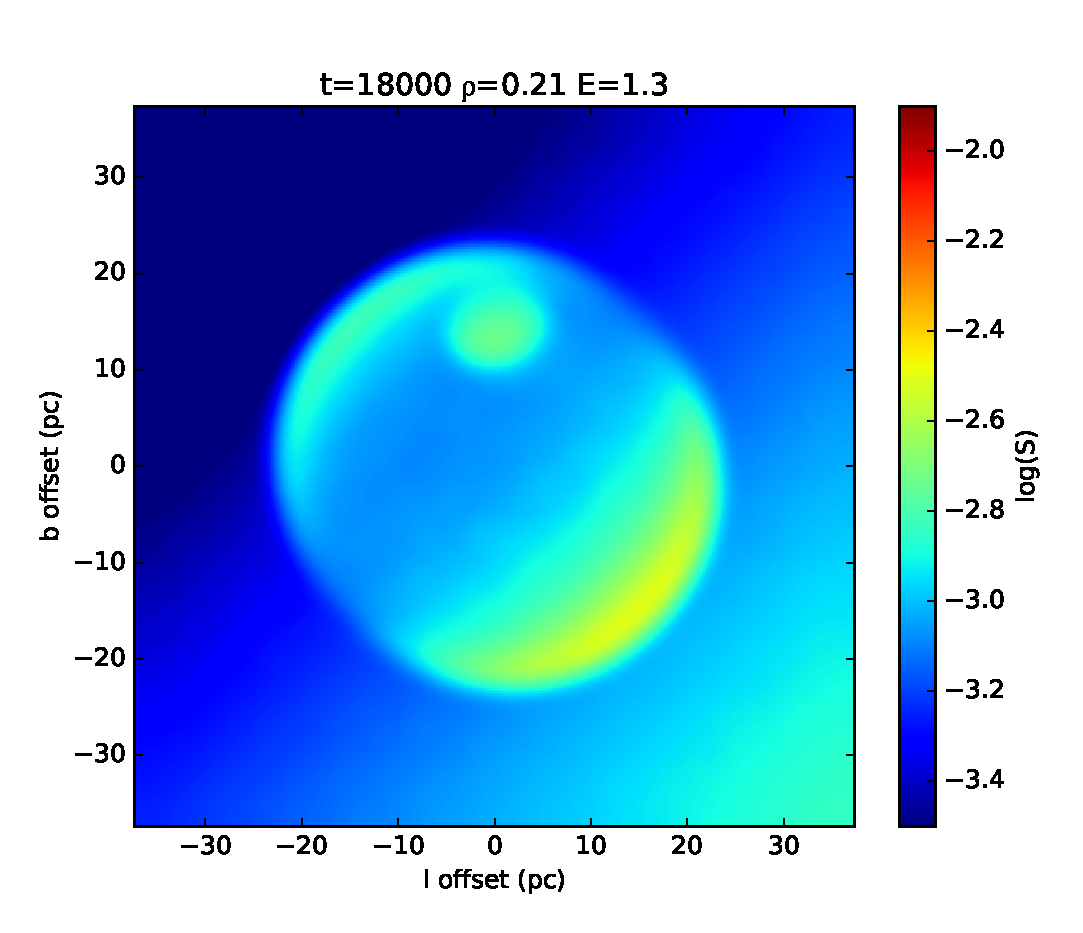
\includegraphics[width=0.472\textwidth]{t18000_density021_E13.eps}
   \caption{左图显示了W51复合区的1420 MHz连续谱图。右图是图~\ref{fig:flux}右图,只是
   改变了颜色风格。取距离为4.3 kpc,两者有相同的大小。}
\label{fig:compare}
\end{figure*}

根据我们模拟的结果,新的壳层流量密度只是西南边的主壳层的一半(见图~\ref{fig:change})。
而主壳层的亮温度大约为60 K(图~\ref{fig:compare}),因为亮温度与流量密度是成正比的,
所以新壳层的亮温度是30 K,这显然大于VGPS观测的灵敏度。
以0.25为谱指数,可以估算出使用Effelsberg 100m望远镜在11cm波段观测主壳层的亮温度是14K,
那么这个新壳层的亮温度就是7K。
W51C主壳层的偏振度在11cm是3$^{+1.8}_{-1.0}\%$ \citep{1974A&A....32..375V},
我们假设新壳层偏振度与此相似,那么新壳层的偏振强度大概是210mK,大于Effelsberg 11cm偏振
巡天的灵敏度。
同时,我们模拟中在东北区域的磁场放大非常明显,也说明真实的偏振流量应该很大。
可是,通常电离氢区在这个波段的偏振辐射几乎是没有的,如果我们在这个区域真的观测到了偏振
辐射,那它应该来源于W51C而不是W51A,也就印证我们模拟的正确性及新壳层的存在。

而图~\ref{fig:mag}真正地揭示了这个区域偏振辐射的存在。
\citet{1974A&A....32..375V}曾经发现W51C的主壳层大部分区域都有偏振辐射,在
图~\ref{fig:mag}的左图中,也就是没有扣除仪器偏振时,我们的确也能看到主壳层的偏振辐射,
可是在扣除仪器偏振的右图中,主壳层的大部分区域偏振辐射消失了,这代表着我们其实多扣了
仪器偏振。
因为仪器偏振在不同情况下有很大的误差,我们只是取的平均值,如果我们多扣了偏振,那么剩下
的偏振辐射只是一个下限,几乎可以肯定不是虚假信号。
此外,大概朝向W51A的仪器偏振\citep{1987A&AS...69..451J}和背景偏振
\citep{1999A&A...350..447D}的方向都与我们在这个区域观测到的偏振方向不同,这说明我们观测
到的偏振的确来自观测到的源。
此外,我们在这个方向也没有观测到其它偏振源\citep{Xu2014}。
而东北和南部区域的磁场方向相似,也与我们的模拟相吻合,既然南部区域的偏振辐射来自W51C,
那么东北部应该也来源于W51C。
而且,\citet{1974A&A....32..375V}估计W51C主壳层在11 cm的总流量密度为51.5 Jy,所以据
我们估计这个新壳层的流量密度为25.7 Jy。
巧合的是,\citet{1994JKAS...27...81M}曾经提到观测W51A时推出其在11 cm有非热的流量密度
28 Jy,与我们的估算相近。
但是,W51A是一个电离氢区,在这个波段不可能有这么强的非热射电辐射,所以他们很困惑这个非热
流量的起源。
所有这些线索都让我们相信,W51C有一个新的之前未被发现的壳层与W51A刚好在视线方向重合。

事实上,大部分超新星都是近似球对称爆发的,所以大部分因为磁场的存在应该演化出两个壳层。
即使在非均匀介质中,我们也很难模拟出单壳层遗迹。

\subsection{相互作用区域}
\citet{1994JKAS...27...81M}估计了小电离氢区G49.2-0.35的在11 cm的非热辐射流量大约为
9 Jy, 而\citet{Brogan2013}的研究也支持这样一个结果,这在当时是令人困惑的。
我们在图~\ref{fig:mag}中也发现这个方向有微弱的射电偏振辐射,这让我们猜想,是否这个区域
的非热辐射也来源于W51C。
这个区域临近W51C的爆发中心,所以这个非热辐射可能是沿着视线方向膨胀的壳层与分子云相互作用
的结果。
通常,如果超新星遗迹球对称爆发,因为光学薄,边界的射电亮度要远远高于中心,类似于太阳的射
电临边增亮效应。
可是,激波与分子云相互作用或许会增大辐射流量密度,从而中心区域也可能有少量可探测的辐射
(如图~\ref{fig:moreflux})。
事实上,我们在这个区域探测到了1720 MHz OH脉泽,这也支持在这个区域有超新星遗迹和分子云
的相互作用。

除此之外,如果激波沿着视线方向与分子云相互作用,在我们看来它不会改变初始的磁场方向。
而在这个区域观测到的磁场方向刚好与我们模拟中假设的方向一致,这也说明我们对磁场方向的假设
是正确的。
另外,银河系大尺度磁场在这个方向与我们观测到的不一致,这说明我们观测到的并不是前景或者
背景的大尺度磁场,而是源本身的磁场。
这个初始磁场可能来源于大质量前身星星风,或者在这颗大质量恒星诞生前,分子云坍缩时就逐渐
形成,而小区域的恒星形成及演化会影响当地的磁场分布,从而导致其与大尺度磁场并不相符。

另一方面,OH分子的合成与其脉泽的产生是完全两个过程。
激波解离分子云中的分子,并在激波后产生OH分子。
而1720 MHz OH脉泽产生的条件更为苛刻,需要合适的温度、密度、OH柱密度。
也就是说,即使有相互作用也不一定有1720 MHz OH脉泽,而有1720 MHz OH脉泽就几乎肯定有相互
作用。
这些脉泽只会在很小的满足条件的区域产生,因而辐射很强的同时,谱线很窄。
结果就是,其实相互作用后产生的大部分区域很多OH分子并不能形成脉泽,这些分子本身也会有一定
发射,但是会很弱,而且谱线很宽。
而如果这些分子的背景有很强的连续谱源,比如电离氢区或超新星遗迹,就会产生吸收谱。
\citet{Hewitt2008}认为我们在这个方向探测到了窄的1720 MHz OH和宽的1667/1665/1612吸收线
是遗迹和分子云相互作用的关键证据。
可是,如果背景的源很弱,我们其实很难观测到吸收线,对于超新星遗迹,只有当产生OH分子的位置
本身也有较强连续谱辐射才会有吸收线。
好在G49.2-0.35方向有这个辐射很强的电离氢区,我们可以观测到很深很宽的吸收线,这或许暗示了
相互作用区域是在G49.2-0.35前方的。
不过,其实电离氢区本身也可以产生OH的吸收和发射线,不同点在于发射线相对SNR产生的要宽一些。

G49.2-0.35距离W51C非常近,因而我们很难通过特征速度判断这些特征到底来源W51C相互作用区域,
还是电离氢区G49.2-0.35。
不过通过分析图~\ref{fig:OH}中的谱形及不同谱的位置,我们或许可以一窥究竟。
在1720 MHz的谱线图中,我们看到脉泽位置是与G49.2-0.35分开的(图~\ref{fig:spectra}中
更明显),这说明1720 MHz OH脉泽与这个电离氢区无关,同时其非常窄的线宽让我们相信这一定是
遗迹分子云相互作用的结果。
再看另外两幅图,有1720 MHz OH脉泽的周围并没有1665/1612 MHz的发射,或许因为OH分子很少,
本来这种沿着视线方向的相互作用产生的辐射流量就不会太大。
可是在距离1720 MHz OH脉泽更远的G49.2-0.35射电弱一些的区域我们看到较强的1665 MHz发射和
微弱的1612 MHz发射(1665/1667 MHz是主跃迁频率,1720/1612 MHz是次跃迁频率,相同情况下
主跃迁的发生概率更高,因而1665/1667 MHz的辐射要强一些)。
这就很奇怪了,如果这些OH线都与W51C有关,理论上1720 MHz OH脉泽附近产生的OH分子应该更可能多
一些,如果这里没有那么多,其它地方应该更少。
考虑到电离氢区也能产生OH,所以我们认为G49.2-0.35方向的OH谱线发射可能更多的与这个电离氢区有
关,而不是W51C。
因而,谱线吸收也更可能与电离氢区有关,结果就是,根据这些我们是无法判断电离氢区G49.2-0.35
与W51C的前后关系的。

图~\ref{fig:spectra}显示这个区域的中心吸收速度与1720 MHz OH脉泽的中心发射速度有微弱的
偏移,而且频率越低偏移越大。
当然,这种偏移很可能有局部运动的影响,可是最大与最小的速度偏差达到了5 \kms,这个偏差大到
足以让我们认为这进一步说明OH谱线吸收与G49.2-0.35有关,与W51C无关。
不过,这个偏差并没有大到让我们能确定G49.2-0.35与W51C的前后关系。
虽然,根据银河系旋转模型,这个方向上速度越小的源越靠近我们,也就是说在我们的谱线上看,如果
局部运动偏差没有超过5 \kms,G49.2-0.35是在W51C前面的,而\citet{Brogan2013}和
\citet{Ginsburg2015}也认为G49.2-0.35是在W51C前面的。

此外,我们看到图~\ref{fig:spectra}的1720 MHz OH脉泽有两个峰,而实际上,这里有三个脉泽
源,其中两个源距离很近而且速度一样\citep{Brogan2013},结果我们只看到了两个峰71和73 \kms。
可是通常如果遗迹与分子云相互作用,我们应该看到相互作用区域有很多1720 MHz OH脉泽
\citep{Wardle2012}。
可是W51C只有这三个脉泽,而且如此集中,这其实与我们模拟中的假设和其它观测不谋而合。
W51C的激波是与分子云沿着视线方向相互作用的,接触面可能还很小,因而脉泽很少,非热辐射很少,
偏振辐射也很少。
而我们认为这个相互作用是正在进行的,所以,如果再过一段时间,或许观测这个区域会出现更多
脉泽,更强非热和偏振辐射。

总之,基于模拟结果,我们认为W51C的激波与分子云在这个区域沿着视线方向相互作用,而偏振辐射、
非热辐射和OH谱线观测都证实了这件事。
这个结论同时也与初始的磁场方向假设及只有少量1720 MHz OH脉泽存在这一事实相符。

\section{总结}
\label{W51Csum}
我们模拟了超新星遗迹W51C从850年到18000年的演化。
我们的模拟结果显示,W51C在东北方存在一个新的壳层,估计这个壳层流量高于VGPS巡天的灵敏度。
通过分析偏振数据并结合前人对其非热辐射的研究,我们认为这个新的壳层的确存在。
此外,我们在一个距离W51C爆发中心很近的小电离氢区G49.2-0.35方向观测到了明显的偏振辐射,
这可以解释为遗迹的激波沿着视线方向与分子云相互作用的结果。
另外,我们研究了这一区域的OH谱线,并认为OH吸收主要来自于G49.2-0.35,而与W51C无关,可是
并不能肯定G49.2-0.35与W51C的前后关系。
最后,我们预言,只要过去足够长时间,G49.2-0.35方向会出现更多脉泽点,更强的非热辐射和
偏振辐射,这主要是因为W51C与分子云的相互作用会逐渐加深。

\chapter{关于超新星遗迹的前身星星风如何影响其射电形态}
\label{SW}

\section{研究历史及意义}
\label{SWintro}
数值模拟是帮助我们理解超新星遗迹演化的重要手段,随着集群计算能力的提升,我们可以做到很多
之前难以做到的模拟。
一开始,对于遗迹的模拟更多是一维流体模拟结合分析解来定性解释遗迹的一些观测特征。
接着,逐渐有很多非常不错的二维流体模拟的工作涌现,尝试研究一些解析解难以描述的磁场放大、
弥漫激波加速和不稳定性\citep{Jun1996,Kang2006,Fang2012}。
而最近,我们已经可以很好的进行三位次流体模拟工作,并将模拟结果转化为射电、光学和X射线图像
以方便与观测相比较\citep{Orlando2007,Meyer2015,Zhang2017},从而帮助我们解释更多观测。
比如,\citet{Orlando2007}注意到有一类遗迹只有单边壳层,然而大部分超新星爆发都可看作球对称,
这是很难通过解析解解释的,于是他们通过假设带周围介质有密度或者磁场梯度的初始条件模拟这一
类遗迹,不过没有解释为什么会存在这样的梯度。
我们在章节~\ref{W51C}也采用了这种设置,但是根据观测密度梯度几乎不可能存在,所以我们
采取假设磁场梯度。


在之前对超新星遗迹W51C的模拟中,我们发现初始的介质分布对模拟结果有很大的影响。
而实际上


\section{模拟模型}
\label{SWmod}

\section{结果和讨论}
\label{SWres}

\section{总结}
\label{SWsum}

\chapter{超新星遗迹在强磁场中的演化}
\label{Mag}

\section{简介}
\label{MagIntro}

在之前对超新星遗迹的模拟中,我们都是使用银河系磁场的典型值,大约9$\mu G$
\citep{Crutcher2012,Haverkorn2015}。
然而实际上,在银河系中心的致密云块中,磁场是可以达到1$mG$的\citep{Ferriere2009}。
当然,这些云块尺度并不是很大,很多相对于SNR来说很小。
不过有一些云块呈长条状,长度甚至超过SNR尺度,当然宽度可能只在1pc的量级。
这些云块很散乱,少量存在或许不会对SNR演化起到很大影响,然而银河系中心其实是大量存在这类
云块的。
这就导致,虽然大部分区域磁场仍然很弱,但是把这些云块考虑在内,平均磁场可能很强。
我们在章节~\ref{TheoryMHD}也提到,磁场会很大程度上影响SNR演化,尤其是其中粒子加速。
可是之前对SNR的研究大多关注在银河系典型磁场中的演化,当然,这其实是比较合理的,
因为银河系大部分区域的磁场还是比较弱的。
但是银河系中心单位体积内超新星爆发概率也比其它地方要高一些,这里的SNR宇宙线加速其实可能
占据整个银河系很大比重。
当然,也有很多人进行过不是针对SNR的在强磁场中的爆发模拟,这些模拟大多是用来测试MHD程序
的性能,物理上并没有解释SNR的性质\citep{Balsara1999, Stone2009, Barnes2018}。

所以,我们认为模拟SNR在强磁场中的演化是非常有必要的,这可以帮助我们理解SNR在银河系中心
的演化,并为解释宇宙线能谱提供一个参考。
不过在我们的实际模拟中发现,强磁场中的SNR形态也是非常不一样的,这可以帮助我们理解上一
章中没有解释清楚的多壳层遗迹。
本章中,我们采用了AMR技术以方便解释更细微的SNR结构和理解磁场在SNR演化中的作用。

\section{参数和结果}
\label{MagMod}
我们主要使用的初始三维网格为64 $\times$ 64 $\times$ 64,不过使用了level为4的AMR技术,
最终网格化效果接近1024 $\times$ 1024 $\times$ 1024。
此外,使用AMR画磁场、速度等矢量比较麻烦,所以我们也做了128 $\times$ 128 $\times$ 128
的模拟,方便看一下大尺度的参数变化。
另外,因为银河系平均介质密度大约为0.5 cm$^{-3}$,而考虑致密云块后的平均密度其实不太好估算,
我们在这里暂且取10 cm$^{-3}$。
作为比较,我们分别模拟了这两个密度下的SNR演化,相对应的,要达到初始半径所需的时间分别
为1881年和693年。
其它具体参数请见~\ref{table:parameters}。

\begin{table}
  \caption{强磁场中SNR模拟参数}
  \label{table:parameters}
  \centering
  \begin{tabular}{l l l}
      \hline\hline
      参数                      & 值            & 参考文献               \\
      \hline
      超新星遗迹参数\\
      \hline
      抛射质量                    & 15.8 M$_{\odot}$ & 1\\
      爆发动能                    & 2.0$\times$ 10$^{51}$ ergs & 2, 3\\
      初始半径                    & 4 pc             &\\
      模拟起始时间                & 1881 $\&$ 693 years        & 4\\
      总模拟时间                  & 10000 years\\
      \hline
      别的参数\\
      \hline
      平均介质数密度 (n)         & 0.5 $\&$ 10 cm$^{-3}$   & 5, 6\\
      磁场强度 (B)              & 900 $\mu$G   & 7, 8\\
      平均原子权重              & 1.3              &\\
      绝热系数                  & 1.7              &\\
      \hline
  \end{tabular}\\
  ~\\
  (1)\citealt{Sukhbold2016}; (2)\citealt{Poznanski2013}; (3)\citealt{Mueller2016a}; (4)\citealt{Leahy2017a};
  (5)\citealt{Nakanishi2006}; (6)\citealt{Nakanishi2016}; (7)\citealt{Haverkorn2015}; (8)\citealt{Ferriere2009}
\end{table}

初步的模拟结果在图~\ref{fig:gc}中,只展示了y-z平面的密度分布图像。
因为直接处理数据得出的矢量图太大,在电子版文章中渲染很慢,我们在这里使用截图后转的矢量图,
部分细节在放大后可能稍有出入。
图中的彩色网格是AMR网格的集中度,越密集的地方网格越多,分辨率也就越高。
另外,图像背景处看似白色的网格其实是软件的图像渲染效果,不是真实的模拟结果。
对密度为0.5 cm$^{-3}$时4500年的图像我们去掉了网格,为了看起来更清晰。
我们发现,无论何种参数,加入强磁场的SNR在演化早期就出现了明显的非球对称演化,而更偏向
于柱对称。
而这在章节~\ref{W51C}中的模拟虽然有一些倾向,但整体还是可以看作球对称的。
另外,我们发现,无论密度高低,SNR中垂直磁场方向的壳层密度更高,而平行磁场方向的壳层密度
更低。
这一现象的起因或许可以从磁场、速度矢量图上得到线索(见图~\ref{fig:low})。
垂直于磁场方向的激波再一开始会压缩磁场,而过一段时间以后,这个方向上会产生较强的反向
激波,反而向爆发中心汇聚。
其实平行于磁场方向的激波也会产生反向激波,只是很弱罢了,这种不同方向产生的反向激波
强度不同的原因自然是磁压的不同。

我们在图~\ref{fig:beta}给出了热压、磁压比$\beta_b$的分布图,很明显垂直磁场运动的激波
会放大磁场,使得$\beta_b$变小,磁压变大,总体压强变大,更容易产生反向激波。
同时,因为磁场很强,其回复力导致最初压缩的磁场慢慢回复原样。
反向激波中的物质逐渐被回复的磁场引导沿着磁场运动,流向两端。
这样一个结果导致,SNR演化大部分的物质都向沿着磁场的两端汇聚,类似喷流的准直效果。
另外,在图~\ref{fig:beta}的右图中可以看出,SNR中最大的$\beta_b$值在1左右,而
最小的值在0.01。
与带入章节~\ref{TheoryMHD}中的方程~\ref{eqn:ratio},可得$\beta_b=1$时,
$M^2=0.5+0.4+4.4=5.3, r=1.2$。
而$\beta_b=0.01$时,$M^2 \approx 40000, r \approx 1$。
其实对这个方程,本来就有$\beta_{b,2}\to 0, r \to 1$,也就是说磁场太强的时候,上下游的
密度、速度几乎不变化。
要注意的是,这并不意味着SNR上游、下游性质一样,无法区分SNR与ISM,而是一种特殊情况。
这里的磁压因为之前的压缩已经很高,本来由激波带来的动压已经无法抵挡住磁压,也就是磁场回复
的倾向。
最终磁场会像我们在模拟中展示的那样恢复到初始状态,这个回复过程必然会产生比没有磁场时更强
的反向激波,这也就是为什么我们在模拟结果中看到磁场回复的同时,反向激波很强的原因。

此外,我们看到低密度的垂直于磁场运动的激波通常比高密度的平行于磁场运动的激波运动更快,
这个也可以用我们之前推导DSA的公式来解释。
垂直于磁场的激波被磁压影响较大,大量物质被反向激波带走,所以密度低,这个很清楚。
同时,其压缩比$r$在某一时刻相对来说更小,这意味着上下游速度的差值更小。
因为这里假设超新星球对称爆发,各个方向激波速度相同,也就是说垂直和平行的激波初始速度相同。
传播过程中,激波因为与介质相互作用而减速,逐渐趋向于上下游速度一样,最终与ISM随机运动速度
一样,从而消散。
而单位时间内减速的多少由压缩比决定,因为上游速度趋向于下游速度,压缩比小意味着上下游
速度更加相近,上游减速越慢。
这里说的上下游是以激波面静止系为基准,如果周围介质在ICRF中静止,那么上游速度就是激波面
在介质中传递的速度。
而垂直于磁场的激波,压缩比总是比较小,上游速度减速也就更慢,激波面的速度也就一直更快,正
如我们在上面几幅图中看到的现象。


\begin{figure*}
    \centering
    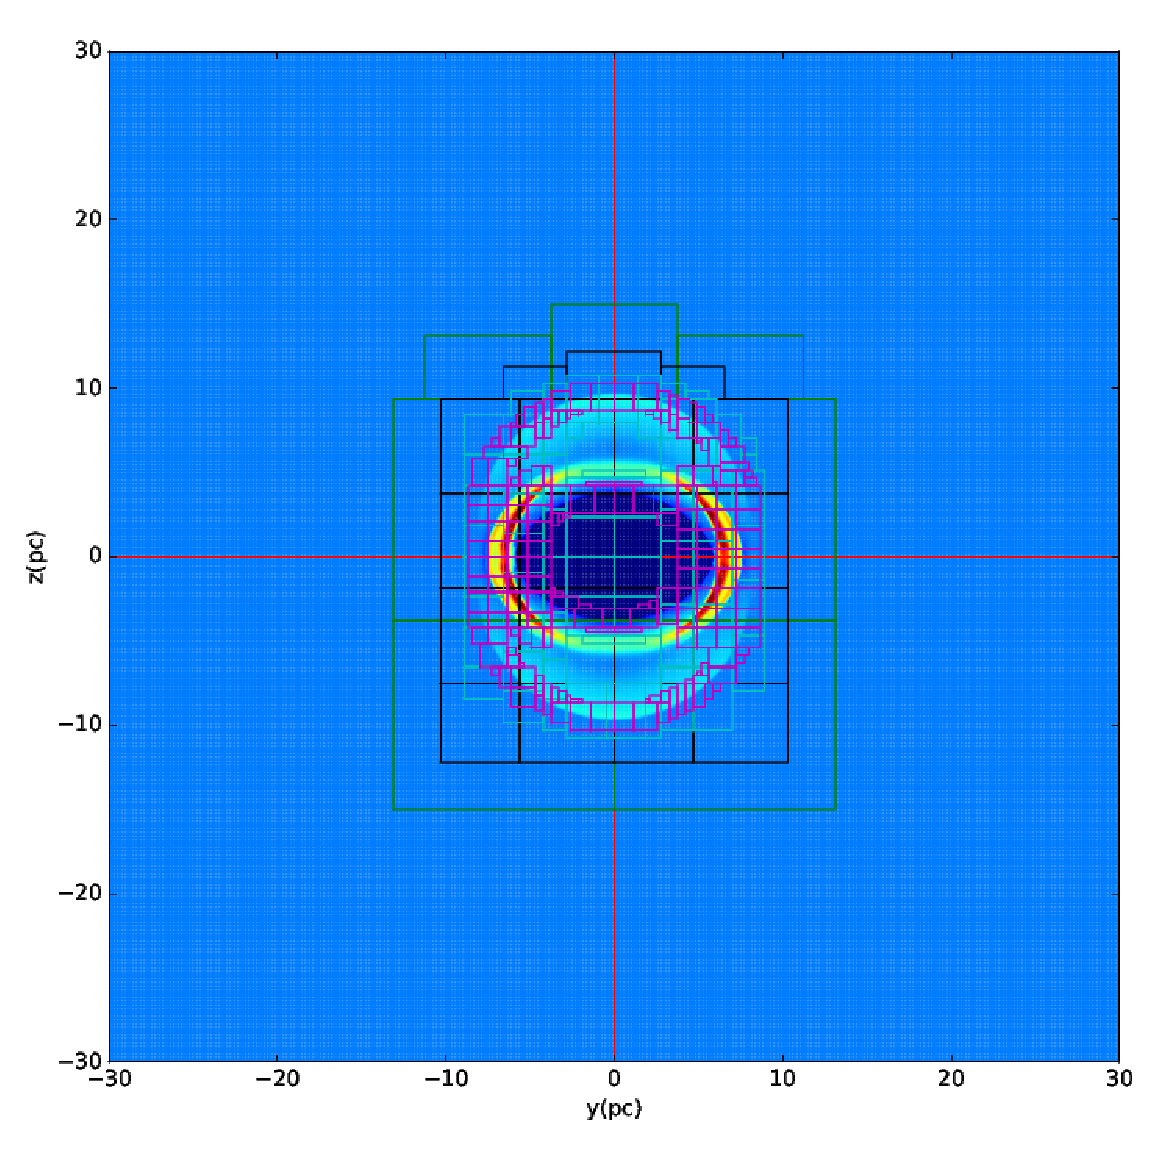
\includegraphics[width=0.455\textwidth]{1500.eps}
    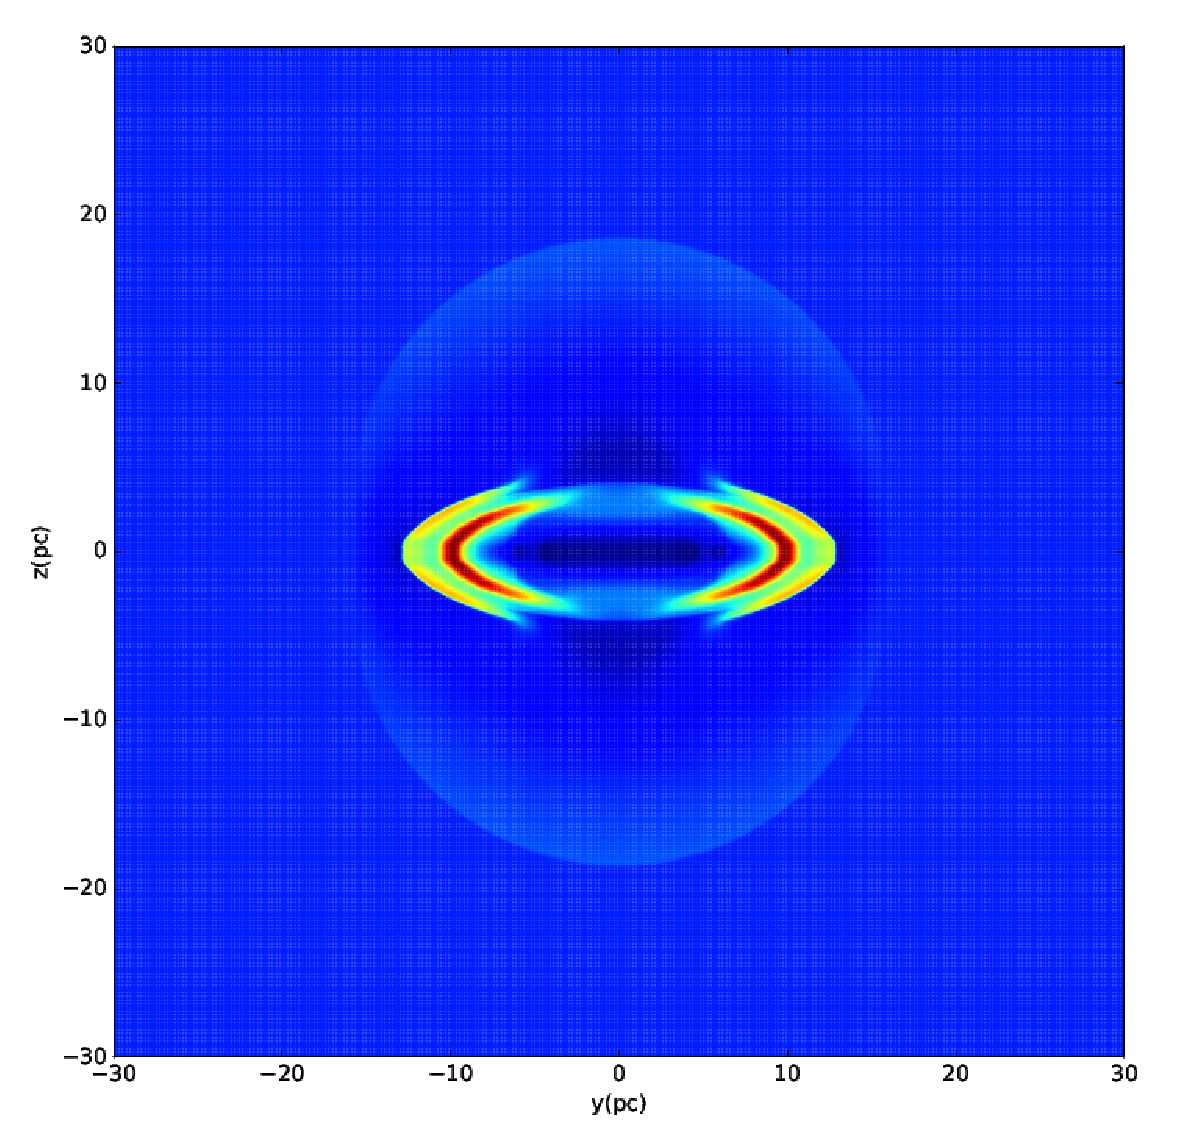
\includegraphics[width=0.455\textwidth]{4500.eps}\newline
    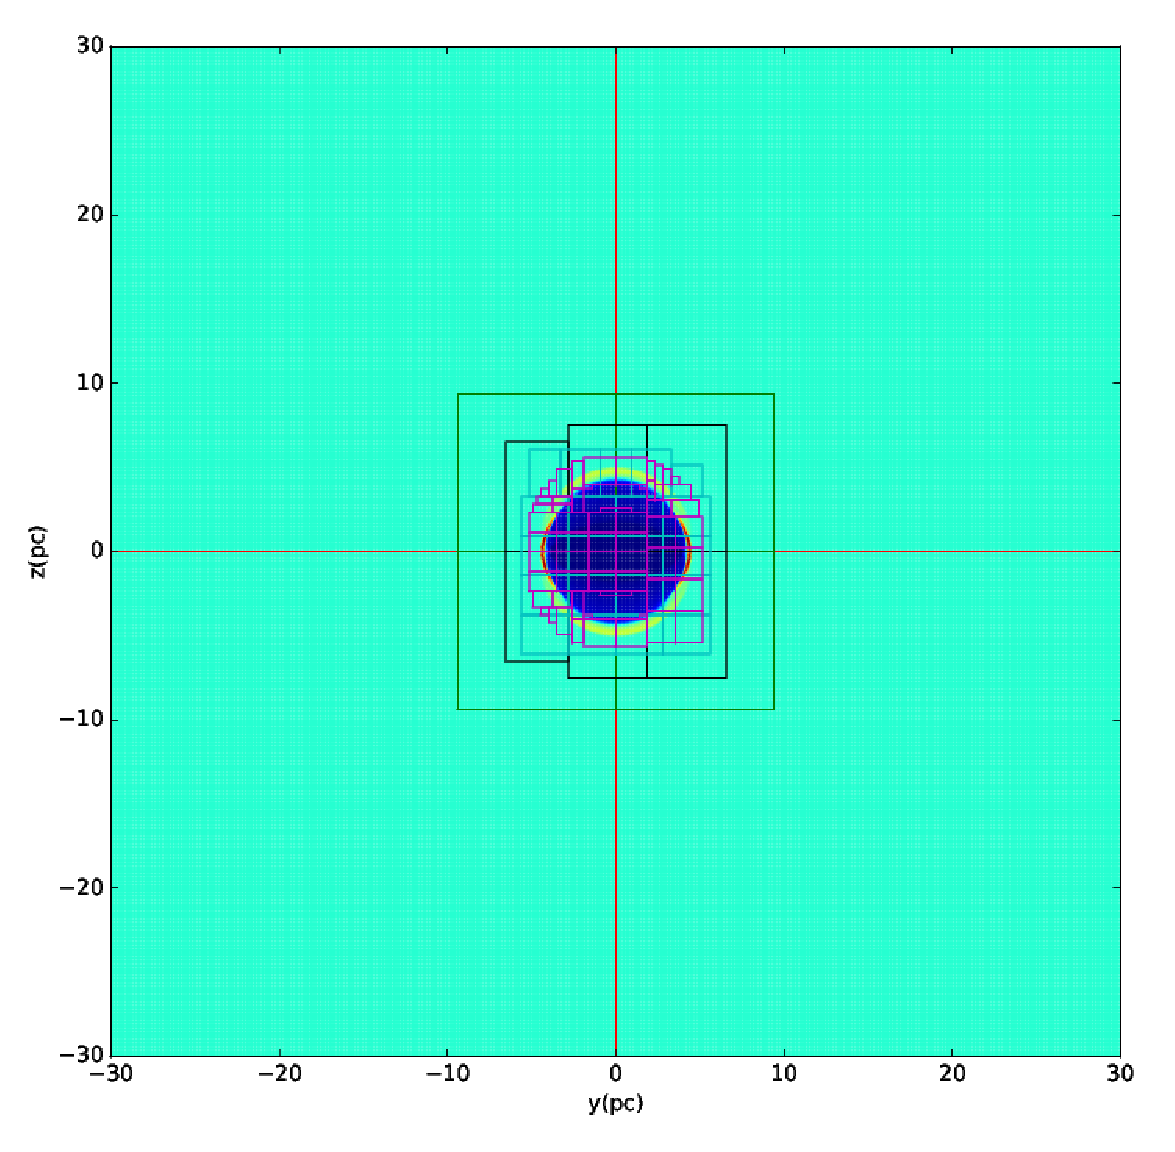
\includegraphics[width=0.455\textwidth]{1500_10.eps}
    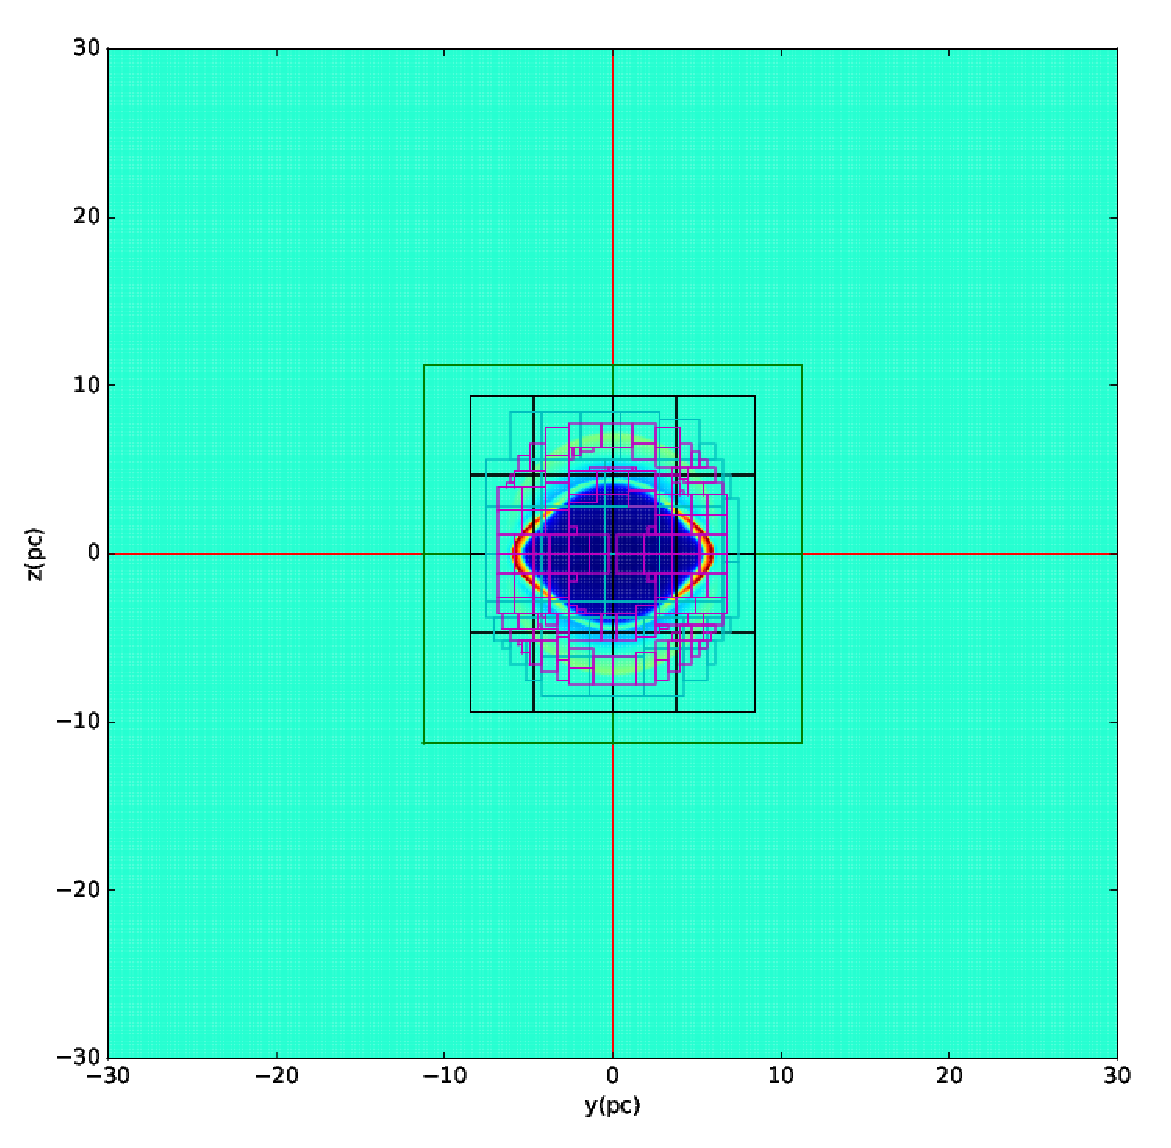
\includegraphics[width=0.455\textwidth]{4500_10.eps}
    \caption{强磁场下的高分辨率模拟的密度分布。上面两幅图是介质密度为0.5 cm$^{-3}$时
    1500年和4500年后的模拟结果。
    下面两幅图是介质密度为10 cm$^{-3}$时1500年和4500年后的模拟结果。
    上下图的真实年龄分别要再加上初始的693年和1881年。}
\label{fig:gc}
\end{figure*}

放在银河系中心考虑这件事就很有意思了。
因为银心处的磁场主要是垂直于银道面的,如果银心过去有过很多超新星爆发,那么这个准直效果
会导致很多物质在银心位置垂直于银道面抛出。
这些抛射物的初始速度至少1000 \kms ,考虑介质作用减速,千万年之后尺度也可达到kpc量级。
虽然,银心引力很强,很多物质受到引力约束,可是实际上银河系年龄也远超千万年,SNR可能
已经消散无法辨别,但是这些抛出的物质应该还可以探测到。
而最近探测到的费米泡(Fermi Bubbles)很可能也会受到这些抛射物的影响。
费米泡能谱是非热的,而最近的研究表明应该是轻子起源,有人猜测是银心黑洞在之前活动时的喷流
导致的\citep{Yang2017},可是实际上非热、轻子起源这些已知条件并不能排除SNR的贡献
\citep{Fujita2013}。

同时,这可以用来解释一些SNR射电与X射线辐射位置的差异问题。
比如SNR G1.9+0.3 \citep{Reynolds2008,Borkowski2017},这可能是银河系中最年轻的遗迹,
因为在银心附近,消光很强,所以爆发时并没有被观测到。
它的SNR射电与X射线形态与我们在这里模拟的很像,对比图~\ref{fig:low}第一张图,
在模拟图像密度高磁场小的相应位置射电辐射很强,而在模拟图像密度低磁场高的相应位置,
X射线辐射很强。
而且,我们看到,当遗迹年龄增大,这种现象会消失。
当然,我们在这里用的参数与G1.9+0.3不一样,未来还要做进一步更有针对性的模拟。

\begin{figure*}
    \centering
    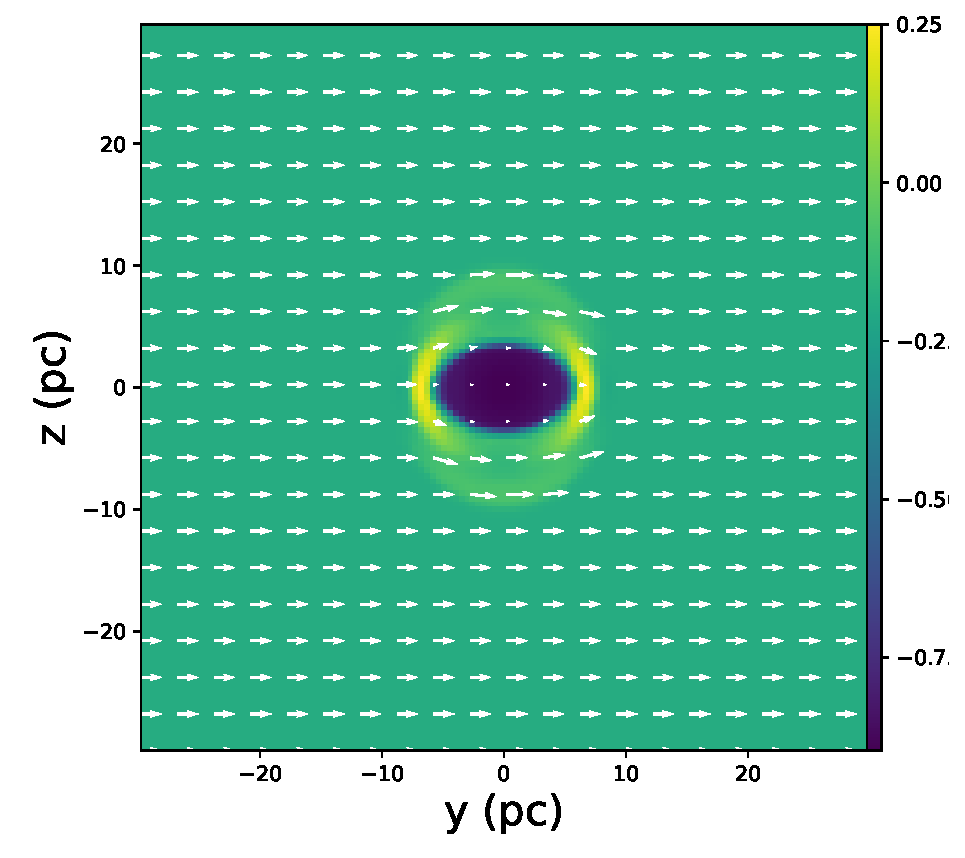
\includegraphics[width=0.455\textwidth]{rho_t3_density1_E1_yz.eps}
    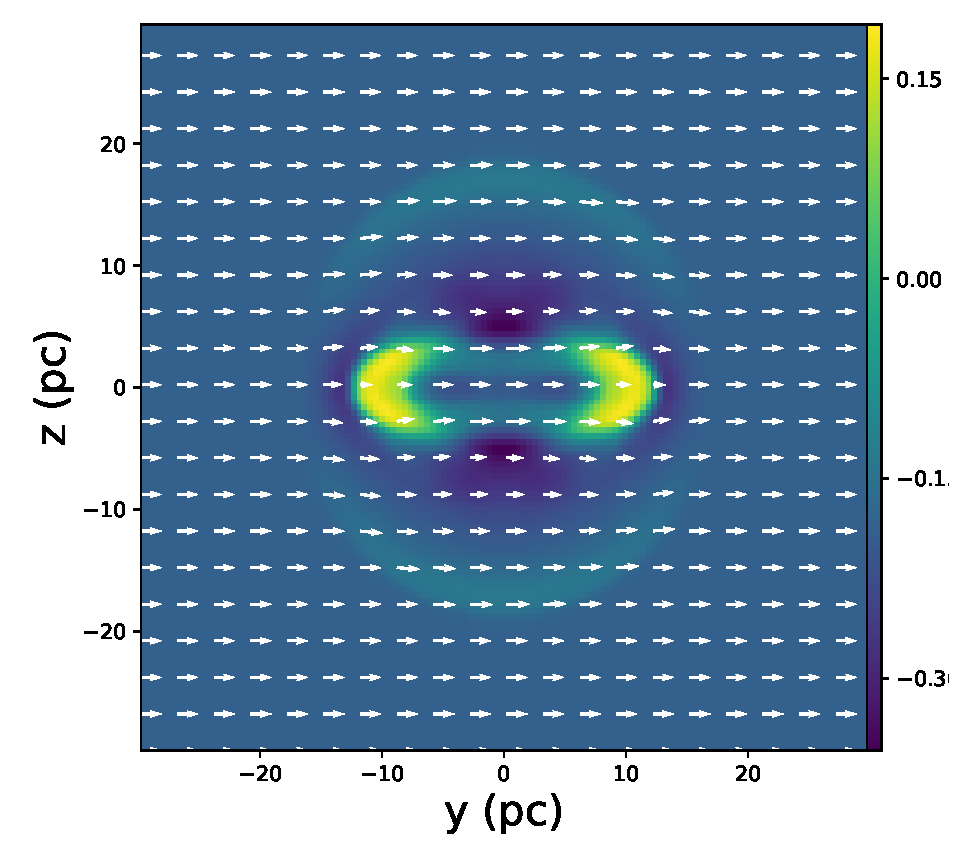
\includegraphics[width=0.455\textwidth]{rho_t9_density1_E1_yz.eps}\newline
    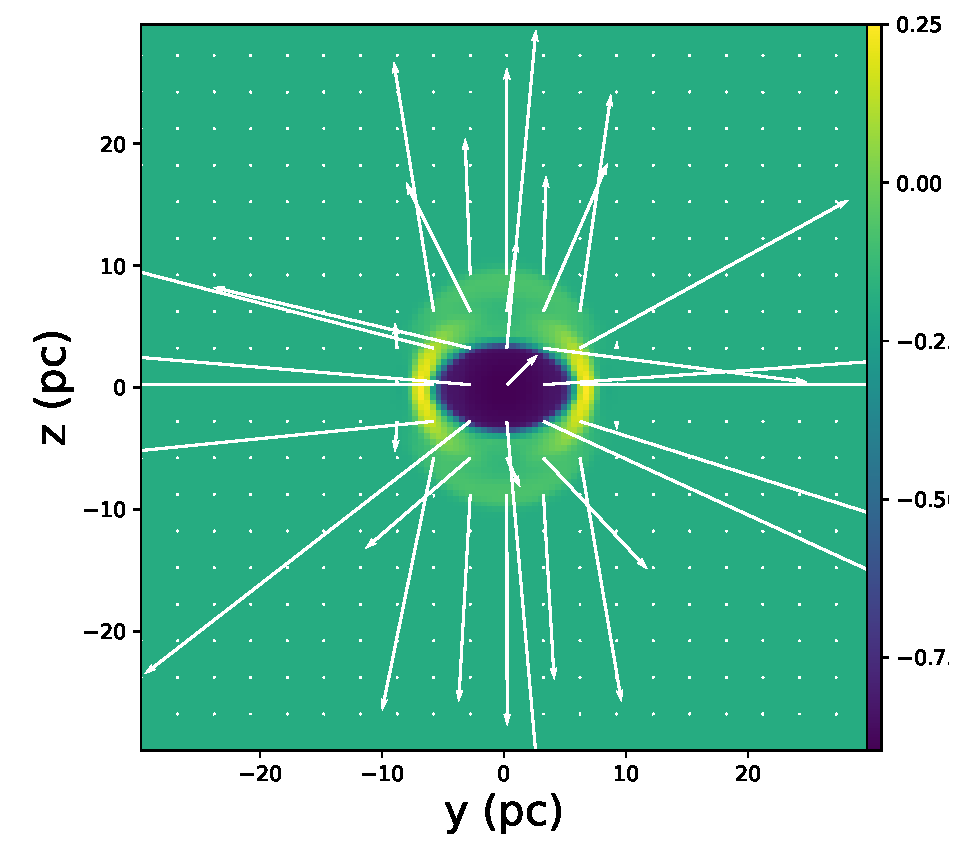
\includegraphics[width=0.455\textwidth]{rhoV_t3_density1_E1_yz.eps}
    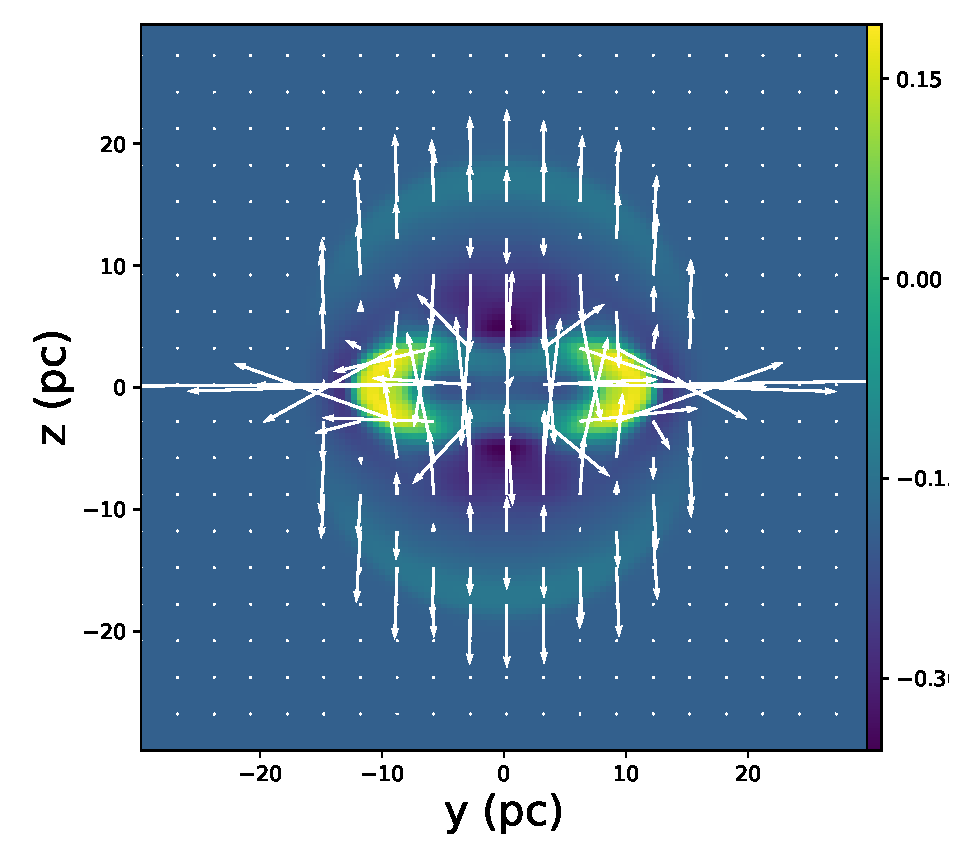
\includegraphics[width=0.455\textwidth]{rhoV_t9_density1_E1_yz.eps}
    \caption{强磁场下的低分辨率模拟的介质密度为0.5 cm$^{-3}$的模拟结果。
    上面两幅图是1500年和4500年后的密度、磁场分布,
    下面两幅图是1500年和4500年后的密度、速度分布。}
\label{fig:low}
\end{figure*}

\begin{figure*}
    \centering
    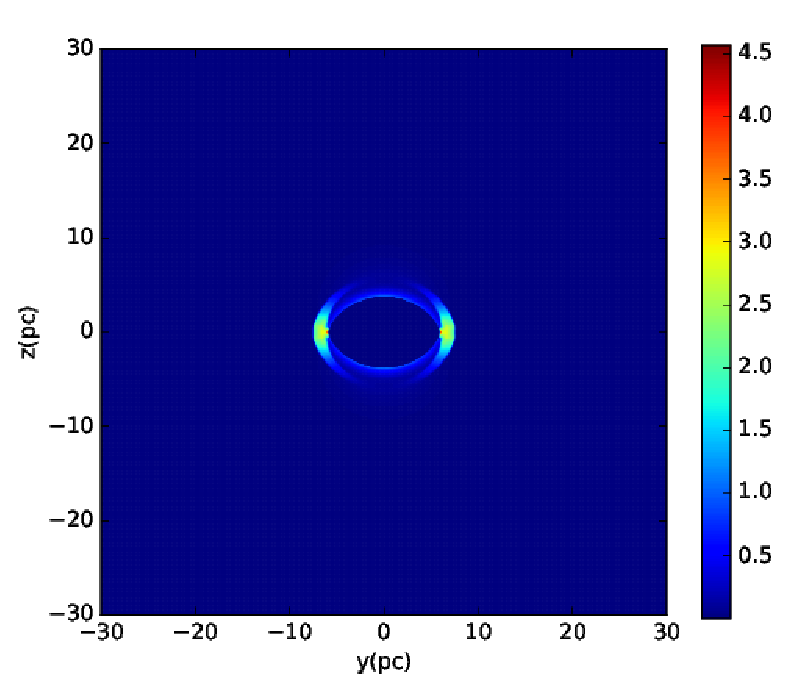
\includegraphics[width=0.455\textwidth]{1500_beta.eps}
    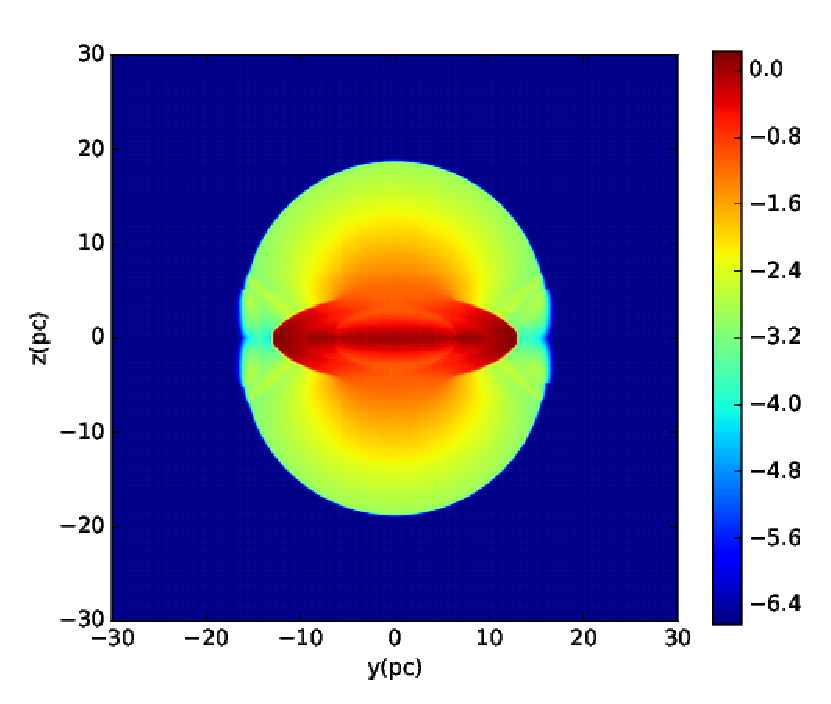
\includegraphics[width=0.455\textwidth]{4500_beta.eps}
    \caption{介质密度为0.5 cm$^{-3}$的$\beta_b$分布。
    左图是1500年后的$\beta_b$分布,右图是4500年后的$log(\beta_b)$分布。}
\label{fig:beta}
\end{figure*}

另外,我们在高分辨率的图~\ref{fig:gc}可看到,高密度区域在出现了一侧双壳层,
这可能主要是来自不同方向的反向激波与正向激波相互作用导致的,或许是章节~\ref{SW}中
多壳层遗迹的一个产生机制。
同时,我们想在这里给10 cm$^{-3}$密度下的演化10000年的结果(见图~\ref{fig:shells})。
这里的确也是出现了多壳层,但却是在相反方向。
所以,我们认为,这种多壳层的产生应该与介质密度、磁场强度、演化年龄,甚至爆发能量、
抛射物质量都有关系。
这些参数之间满足一种关系时才会产生多壳层,而目前这种关系还不明确。

\begin{figure*}
    \centering
    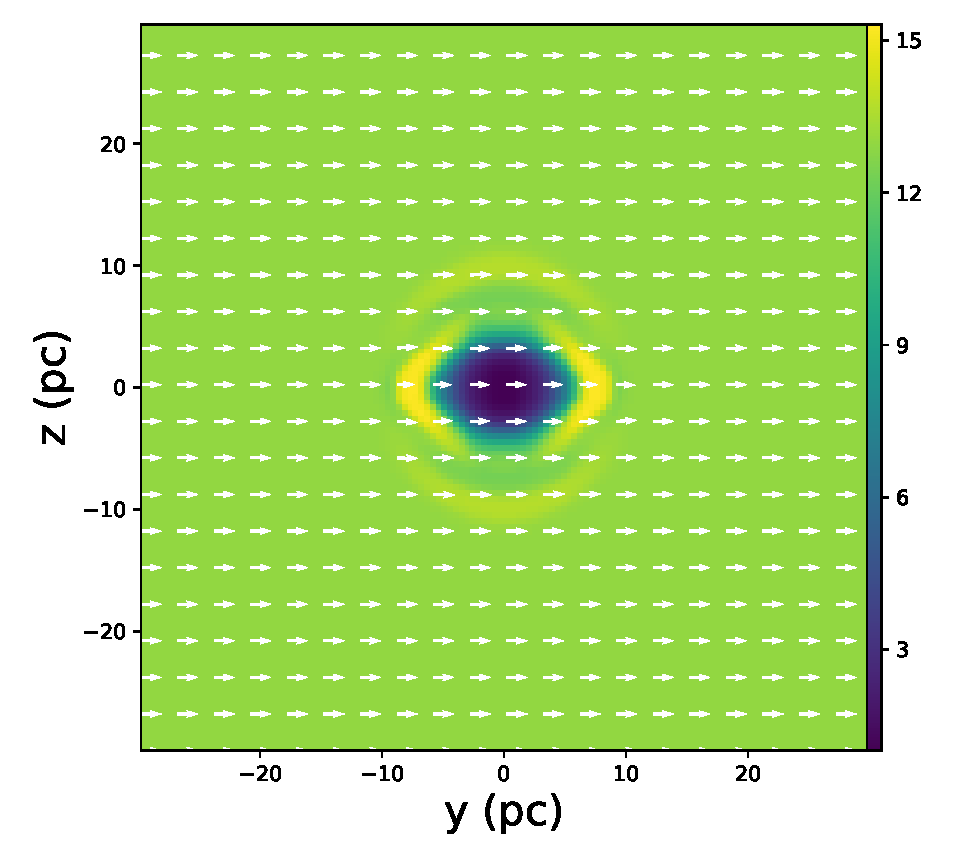
\includegraphics[width=0.475\textwidth]{rho_t20_density1_E1_yzR.eps}
    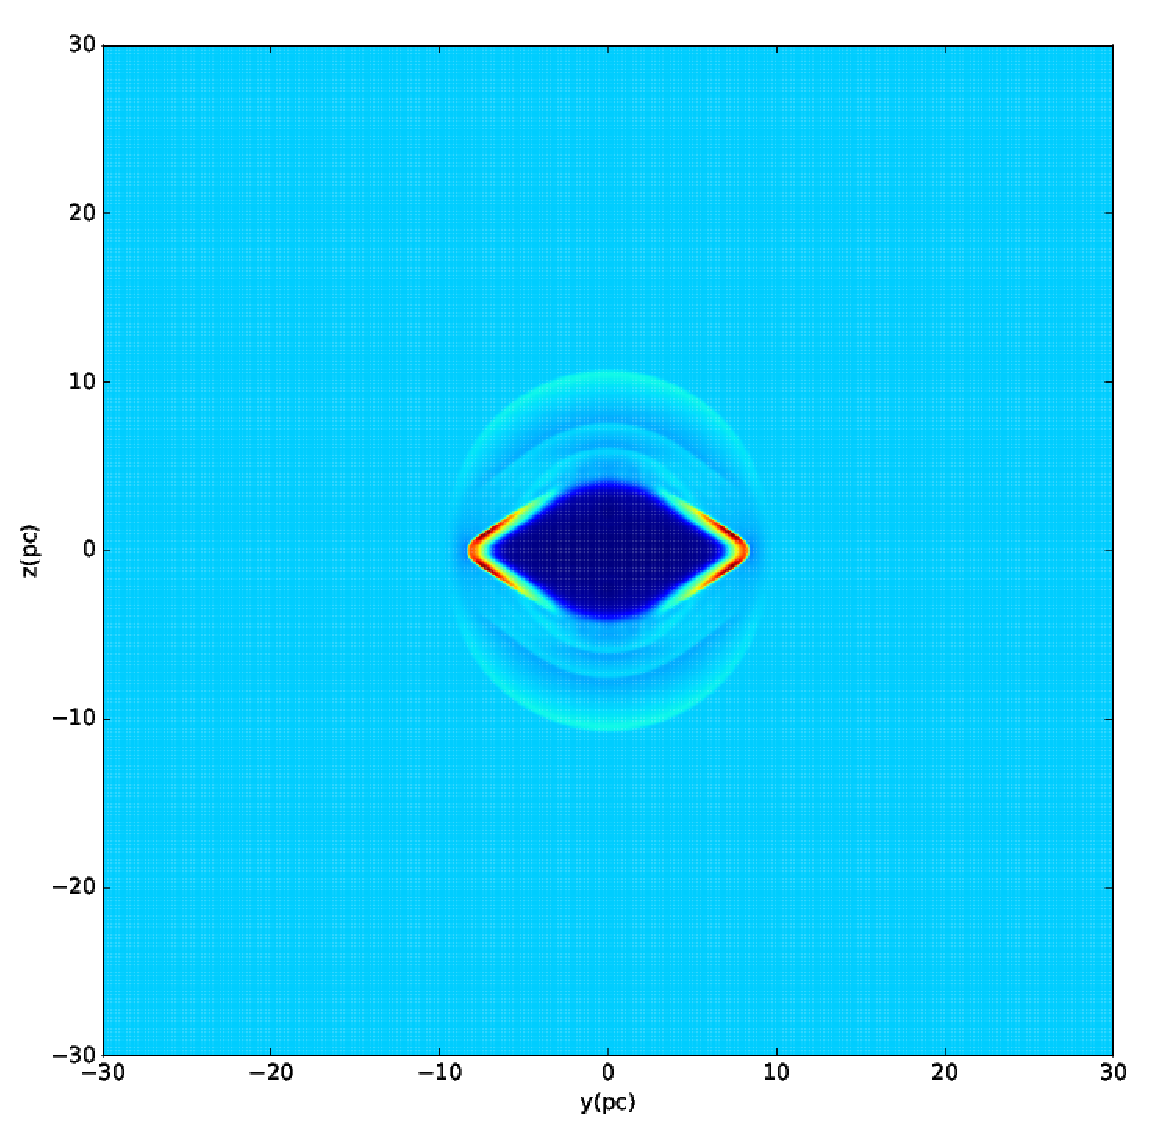
\includegraphics[width=0.435\textwidth]{10000_10.eps}
    \caption{介质密度为10 cm$^{-3}$的10000年演化结果。
    左图是低分辨率包含磁场方向的图像,右图是高分辨率真正出现多壳层的图像。}
\label{fig:shells}
\end{figure*}

\section{总结}
\label{MagSum}

我们在这一部分主要模拟了SNR在强磁场中的的演化,并得到了一些有用的信息:

\begin{enumerate}

    \item 强磁场中反向激波行为在不同方向存在很大差异,形成类似于喷流准直的现象。

    \item 这种准直现象在银河系中心或许会影响到费米泡的形成。

    \item 强磁场中演化的SNR也更有可能出现奇怪的射电和X射线图像,这或许可以解释
    G1.9+0.3的形态。

    \item 多壳层超新星遗迹在强磁场环境中容易出现,可实际形成机理与很多因素相关。

\end{enumerate}

要研究费米泡的形成,还需要大尺度又局部高分辨率的模拟,对计算性能要求很高。
另外,要解决G1.9+0.3的射电、X射线形态问题,以及多壳层的产生问题,需要调整多种参数
组合做测试,同样需要大量工作。

\chapter{总结}
\label{Sum}

我们在本文中首先介绍了超新星遗迹的流体演化模型和辐射特性,并详细阐述了扩散激波加速机制的
具体理论和局限,并以此为基础说明宇宙线的起源和SNR中的各种辐射机制。
经典扩散激波加速机制的重要局限之一就是没有考虑磁场,所以我们接着讨论了磁场在激波加速中的
重要性,并尝试得出了考虑磁场的DSA模型,并借此引出我们在实际模拟中需要知道的一些的磁流体特
性的讨论。
然后我们希望,本文可以帮助他人了解具体磁流体模拟编程的细节,因而以比较流行的模拟软件PLUTO
为例介绍了软件使用中须知的各种参数、不同文件的编写以及一些新技术的使用,同时提供了示例代码
供大家参考。

最后我们展示了超新星遗迹在各种不同星周环境中的磁流体模拟,主要结论如下:

\begin{enumerate}

    \item SNR W51C在东北方存在一个新的壳层,之前因为W51A辐射遮挡而未被发现。

    \item 电离氢区G49.2-0.35中的非热辐射和偏振辐射来自于W51C与视线方向上分子云相互作用。

    \item 电离氢区G49.2-0.35附近的OH吸收主要来自于G49.2-0.35,而与W51C无关。

    \item 大质量前身星的星风对超新星遗迹的射电形态有很大影响,可能比最初的周围环境影响
    还大。

    \item 将星风考虑在内,我们可以解释很多遗迹的射电形态,除了多层和不规则遗迹。

    \item 根据模拟结果,我们不建议通过超新星遗迹的射电图像推测大尺度的磁场和密度分布。

    \item 热传导或许会稍微影响遗迹的射电形态,但是并不是非常重要。

    \item 某些遗迹的射线壳层与X射线辐射的偏离可能是因为前身星的运动。

    \item 强磁场中反向激波行为在不同方向存在很大差异,形成类似于喷流准直的现象。

    \item 这种准直现象在银河系中心或许会影响到费米泡的形成。

    \item 强磁场中演化的SNR也更有可能出现奇怪的射电和X射线图像,这或许可以解释
    G1.9+0.3的形态。

    \item 多壳层超新星遗迹在强磁场环境中容易出现,可实际形成机理与很多因素相关。

\end{enumerate}

这些工作中遇到的问题也很多,有的需要观测进一步证实,有的则需要更高分辨率、更大尺度的模拟,
有的需要很多次调参测试。
我们下一步比较倾向于研究费米泡是否可以用SNR演化来解释,这个相比其它问题而言,更多是计算
性能的限制,如果能使用更高性能的集群将会提供很大帮助。

%---------------------------------------------------------------------------%
% main content
%-
%-> Appendix
%-
\cleardoublepage%
\appendix% initialize the environment
\chapter{基本代码}
\label{Basic}

\section{definition.h}
\label{def}
\begin{lstlisting}
#define  PHYSICS                 MHD
#define  DIMENSIONS              3
#define  COMPONENTS              3
#define  GEOMETRY                CARTESIAN
#define  BODY_FORCE              NO
#define  COOLING                 NO
#define  RECONSTRUCTION          LINEAR
#define  TIME_STEPPING           RK2
#define  DIMENSIONAL_SPLITTING   NO
#define  NTRACER                 0
#define  USER_DEF_PARAMETERS     14

/* -- physics dependent declarations -- */

#define  EOS                     IDEAL
#define  ENTROPY_SWITCH          NO
#define  DIVB_CONTROL            CONSTRAINED_TRANSPORT
#define  BACKGROUND_FIELD        NO
#define  RESISTIVITY             NO
#define  THERMAL_CONDUCTION      NO
#define  VISCOSITY               NO
#define  ROTATING_FRAME          NO

/* -- user-defined parameters (labels) -- */

#define  E_EJ                    0
#define  M_EJ                    1
#define  R_EJ                    2
#define  N_H                     3
#define  U_AM                    4
#define  S_PI                    5
#define  N_PI                    6
#define  W_C                     7
#define  BMAG                    8
#define  THETA                   9
#define  PHI                     10
#define  GAMMA                   11
#define  Temp                    12
#define  NU_VISC                 13

/* [Beg] user-defined constants (do not change this line) */

#define  UNIT_DENSITY            CONST_mp
#define  UNIT_LENGTH             CONST_pc
#define  UNIT_VELOCITY           1.0e9
#define  ADD_TURBULENCE          YES

/* [End] user-defined constants (do not change this line) */

/* -- supplementary constants (user editable) -- */

#define  INITIAL_SMOOTHING         NO
#define  WARNING_MESSAGES          NO
#define  PRINT_TO_FILE             NO
#define  INTERNAL_BOUNDARY         NO
#define  SHOCK_FLATTENING          NO
#define  CHAR_LIMITING             YES
#define  LIMITER                   VANLEER_LIM
#define  CT_EMF_AVERAGE            ARITHMETIC
#define  CT_EN_CORRECTION          YES
#define  ASSIGN_VECTOR_POTENTIAL   YES
#define  UPDATE_VECTOR_POTENTIAL   NO

\end{lstlisting}

\section{init.c}
\label{init}
\begin{lstlisting}

  #include "pluto.h"
  #include "math.h"
  #include "time.h"
  #include "stdlib.h"
  #include "stdio.h"
  /* ********************************************************************* */
  void Init (double *us, double x1, double x2, double x3)
  /*
   *
   *
   *
   *********************************************************************** */
  {
    static int first_call = 1;
    double r, theta, phi, B0, E_ej, M_ej, R_ej, n_h, w_c, s, n, n_ISM, r_c, T, u, g_gamma;
    double fnc, alpha, v_ej, t, rho_ch, R_ch, eta, ph, l, up, down;
    E_ej    = g_inputParam[E_EJ];         //爆发能量
    M_ej    = g_inputParam[M_EJ];         //爆发质量
    R_ej    = g_inputParam[R_EJ];         //爆发半径
    n_h     = g_inputParam[N_H];          //氢数密度
    u       = g_inputParam[U_AM];            //介质总体数密度,U是平均分子权重
    w_c     = g_inputParam[W_C];          //激波区质量与爆发总质量之比
    n       = g_inputParam[N_PI];            //激波区密度幂指数
    s       = g_inputParam[S_PI];            //激波区速度幂指数
    n_ISM   = n_h*u;                     //激波前均匀介质区数密度
    T       = g_inputParam[Temp];         //初始温度
    g_gamma = g_inputParam[GAMMA];        //绝热系数

    r_c     = R_ej*w_c;
    fnc     = 3.0/4.0/CONST_PI*(1.0-n/3.0)/(1.0-n/3.0*pow(w_c,3.0-n));
    alpha   = (3.0-n)/(5.0-n)*(pow(w_c,n-5.0)-n/5.0)/(pow(w_c,n-3.0)-n/3.0)*pow(w_c,2);
    v_ej    = pow(E_ej/(M_ej*alpha*0.5),0.5);
    t       = R_ej/v_ej;
    rho_ch  = M_ej/pow(R_ej,3);
    R_ch    = pow(M_ej,1.0/3.0)*pow(n_ISM,-1.0/3.0);

    ph      = 1.1;  //n=0
    l       = 0.343;
  //  up      = 1 + (n-3)/3*pow(phi/l*fnc,0.5)*pow(R_ej,1.5)
  //  down    = 1 + (n/3)*pow(phi/l*fnc,0.5)*pow(R_ej,1.5)
  //  eta     = up/down

  //  rho_c   = (1-eta)*M_ej/(4/3*CONST_PI*pow(r_c,3)); //激波后均匀介质区密度
  //  C       = 2.0*CONST_PI*pow(r_c,n)*rho_c*pow(R_ej,-2*s);
  //  index   = 2*s+3-n;
  //
  //  part1   = C/pow(r_c,n)*pow(r_c,2*s+3)/(2*s+3);
  //  part2   = C*(pow(R_ej,index)-pow(r_c,index))/index;
  //  v0      = pow(E_ej,0.5)*pow(part1+part2,-0.5);

    r = D_EXPAND(x1*x1, + x2*x2, + x3*x3);
    r = sqrt(r);

    us[RHO] = n_ISM;
    us[VX1] = 0.0;
    us[VX2] = 0.0;
    us[VX3] = 0.0;
    us[PRS] = n_ISM*CONST_kB*T/1.67e-6;

    #if ADD_TURBULENCE == YES
    if (first_call){
      int k, input_var[200];
      for (k = 0; k< 200; k++) input_var[k] = -1;
      input_var[0] = RHO;
      input_var[1] = BX1;
      input_var[2] = BX2;
      input_var[3] = BX3;
      input_var[4] = -1;
      InputDataSet ("./grid0.out",input_var);
      InputDataRead("./rho0.dbl"," ");
      first_call = 0;
    }
    InputDataInterpolate(us, x1, x2, x3);  /* -- interpolate density from
                                                input data file -- */
    #endif
  /*
    if (r > 2.5 && r <= 3)
    {
      us[RHO] = 60*pow(r/r_c,0.0);
    }
  */

    if (r <= r_c && r != 0)
    {
      up      = 1.0 + (n-3.0)/3.0*pow(ph/l*fnc,0.5)*pow(r/R_ch,1.5);
      down    = 1.0 + (n/3.0)*pow(ph/l*fnc,0.5)*pow(r/R_ch,1.5);
      eta     = up/down;
  //    eta     = 1.0;
      us[RHO] = rho_ch*fnc*pow(w_c,-n);
      us[VX1] = (x1/t)*eta;
      us[VX2] = (x2/t)*eta;
      us[VX3] = (x3/t)*eta;
      us[PRS] = rho_ch*fnc*pow(w_c,-n)*CONST_kB*T/1.67e-6;
    }

    if (r >  r_c && r <= R_ej)
    {
     // us[RHO] = a[(int) fabs(x1*x2*100)]*rho_c*pow(r/r_c,-n);
      up      = 1.0 + (n-3.0)/3.0*pow(ph/l*fnc,0.5)*pow(r/R_ch,1.5);
      down    = 1.0 + (n/3.0)*pow(ph/l*fnc,0.5)*pow(r/R_ch,1.5);
      eta     = up/down;
  //    eta     = 1.0;
      us[RHO] = rho_ch*fnc*pow(r/R_ej,-n);
      us[VX1] = (x1/t)*eta;
      us[VX2] = (x2/t)*eta;
      us[VX3] = (x3/t)*eta;
      us[PRS] = rho_ch*fnc*pow(r/R_ej,-n)*CONST_kB*T/1.67e-6;
    }

  //  printf("%e\n",eta);
    //theta = g_inputParam[THETA]*CONST_PI/180.0;
    //phi   =   g_inputParam[PHI]*CONST_PI/180.0;
    B0    = g_inputParam[BMAG];

    //us[BX1] = B0*sin(theta)*cos(phi);
    //us[BX2] = B0*sin(theta)*sin(phi);
    //us[BX3] = 0.0;

    #if GEOMETRY == CARTESIAN
     us[AX1] = 0.0;
     us[AX2] =  us[BX3]*x1;
     us[AX3] = -us[BX2]*x1 + us[BX1]*x2;
    #elif GEOMETRY == CYLINDRICAL
     us[AX1] = us[AX2] = 0.0;
     us[AX3] = 0.5*us[BX2]*x1;
    #endif

    #if BACKGROUND_FIELD == YES
     us[BX1] = us[BX2] = us[BX3] =
     us[AX1] = us[AX2] = us[AX3] = 0.0;
    #endif

  }
  /* ********************************************************************* */
  void Analysis (const Data *d, Grid *grid)
  /*
   *
   *
   *********************************************************************** */
  {

  }
  /* ********************************************************************* */
  void UserDefBoundary (const Data *d, RBox *box, int side, Grid *grid)
  /*
   *
   *********************************************************************** */
  {
  }
  #if BACKGROUND_FIELD == YES
  /* ********************************************************************* */
  void BackgroundField (double x1, double x2, double x3, double *B0)
  /*!
   * Define the component of a static, curl-free background
   * magnetic field.
   *
   *********************************************************************** */
  {
  /*
    static int first_call = 1;
    double theta, phi;
    static double sth,cth,sphi,cphi;

    if (first_call){
      theta = g_inputParam[THETA]*CONST_PI/180.0;
      phi   =   g_inputParam[PHI]*CONST_PI/180.0;
      sth   = sin(theta);
      cth   = cos(theta);
      sphi  = sin(phi);
      cphi  = cos(phi);
      first_call = 0;
    }
    EXPAND(B0[IDIR] = g_inputParam[BMAG]*sth*cphi; ,
           B0[JDIR] = g_inputParam[BMAG]*sth*sphi; ,
           B0[KDIR] = g_inputParam[BMAG]*cth;)

  /*
    theta = g_inputParam[THETA]*CONST_PI/180.0;
    phi   =   g_inputParam[PHI]*CONST_PI/180.0;

    B0[IDIR] = g_inputParam[BMAG]*sin(theta)*cos(phi);
    B0[JDIR] = g_inputParam[BMAG]*sin(theta)*sin(phi);
    B0[KDIR] = g_inputParam[BMAG]*cos(theta);
  */

  }
  #endif

\end{lstlisting}

\section{pluto.ini}
\label{plu}

\begin{lstlisting}
[Grid]

X1-grid    1    -37.5    256    u    37.5
X2-grid    1    -37.5    256    u    37.5
X3-grid    1    -37.5    256    u    37.5

[Chombo Refinement]

Levels           4
Ref_ratio        2 2 2 2 2
Regrid_interval  2 2 2 2
Refine_thresh    0.3
Tag_buffer_size  3
Block_factor     4
Max_grid_size    32
Fill_ratio       0.75

[Time]

CFL              0.4
CFL_max_var    1.1
tstop            300.0
first_dt         1.e-2

[Solver]

Solver         hll

[Boundary]

X1-beg        outflow
X1-end        outflow
X2-beg        outflow
X2-end        outflow
X3-beg        outflow
X3-end        outflow

[Static Grid Output]

uservar    0
dbl        60  -1   single_file
flt       -1.0  -1   single_file
vtk       -1.0  -1   single_file
tab       -1.0  -1
ppm       -1.0  -1
png       -1.0  -1
log        5
analysis  -1.0  -1

[Chombo HDF5 output]

Checkpoint_interval  -1.0  0
Plot_interval         1.0  0

[Parameters]

E_EJ                 26.45
M_EJ                 445.25
R_EJ                 4
N_H                  0.21
U_AM                 1.3
S_PI                 1.0
N_PI                 0
W_C                  0.1
BMAG                 2.0e-3
THETA                90.0
PHI                  90.0
GAMMA                1.7
Temp                 1.0e2
NU_VISC              3.87e-9

\end{lstlisting}


\chapter{工具型代码}
\label{Code}

\section{单位制计算}
\label{Codeu}


\begin{lstlisting}
from astropy import units as un
from astropy import constants as con
import numpy as np

#====================单位计算====================

UNIT_DENSITY = 1*con.m_p/un.cm**3
UNIT_LENGTH  = 1*un.pc
UNIT_VELOCITY= 1e4*un.km/un.s
UNIT_B = (UNIT_VELOCITY*np.sqrt(4*np.pi*UNIT_DENSITY)).to(un.g**0.5*un.cm**-0.5*un.s**-1).value*un.G
UNIT_t = UNIT_LENGTH/UNIT_VELOCITY
UNIT_P = UNIT_DENSITY*UNIT_VELOCITY**2
UNIT_M = UNIT_DENSITY*UNIT_LENGTH**3
UNIT_E = UNIT_M*UNIT_VELOCITY**2
#UNIT_B = ((UNIT_E/UNIT_LENGTH**3)**0.5).value*un.G
UNIT_NU= UNIT_P*UNIT_t
UNIT_G = (UNIT_VELOCITY/UNIT_LENGTH)**2/UNIT_DENSITY

#===============输入需要转换的参量================

n   = 0.21*con.m_p/un.cm**3
l   = 4*un.pc
v   = 490*un.km/un.s
B   = 9*un.uG
t   = 1000*un.yr
P   = 1*un.Ba
E_th= 0.96*un.erg
E   = 2.0e51*un.erg
M   = 15.9*con.M_sun
nu  = 2*un.uPa*un.s
G   = 1*con.G

#=================开始转换========================

n   /= UNIT_DENSITY
l   /= UNIT_LENGTH
v   /= UNIT_VELOCITY
B   /= UNIT_B
t   /= UNIT_t
P   /= UNIT_P
E   /= UNIT_E
M   /= UNIT_M
nu  /= UNIT_NU
G   /= UNIT_G

#================输出结果=========================

print('n = ', n.to('').value, '\n'
      'l = ', l.to('').value, '\n'
      'v = ', v.to('').value, '\n'
      'B = ', B.to('').value, '\n'
      't = ', t.to('').value, '\n'
      'P = ', P.to('').value, '\n'
      'E = ', E.to('').value, '\n'
      'M = ', M.to('').value, '\n'
      'nu = ', nu.to('').value, '\n'
      'G = ', G.to('').value, '\n'
      )

\end{lstlisting}


\section{构造初始背景}
\label{Codeb}

\begin{lstlisting}

import numpy as np
import time as ti
from astropy.io import fits

#=====================加入星风==================

def stellar_wind(wdir,number):
    import pyPLUTO as pp
    pp.nlast_info(w_dir=wdir)
    D = pp.pload(number,w_dir=wdir)
    print(D.rho.shape)

    rho = D.rho
    bx1 = D.bx1
    bx2 = D.bx2
    bx3 = D.bx3
    vx1 = D.vx1
    vx2 = D.vx2
    vx3 = D.vx3

    rho = np.transpose(rho)
    bx1 = np.transpose(bx1)
    bx2 = np.transpose(bx2)
    bx3 = np.transpose(bx3)
    vx1 = np.transpose(vx1)
    vx2 = np.transpose(vx2)
    vx3 = np.transpose(vx3)

    return rho,bx1,bx2,bx3,vx1,vx2,vx3

#==================加入磁场====================

def toff(f):
    def wrapper(*args):
        start = ti.time()
        f(*args)
        end   = ti.time()
        print(end-start)
    return wrapper

def f(i,j,k):
    return i*2+j*2

#@toff
def magnetism(width):
    x = np.fromfunction(f,(width,width,width))/500000
    x = np.rot90(x,k=1)
    x = np.transpose(x)
    x = np.reshape(x,width**3,1)
    x = x + 0.001
    return x*0, x, x

#=================组合背景=====================

def combine(components,infilename,outfilename,width,index,rho_constant,sw,clump,mag):
    if 'sw' in components:
        wdir,number = sw
        rho,bx1,bx2,bx3,vx1,vx2,vx3    = stellar_wind(wdir,number)

        rho       = np.reshape(rho,(1,width**3))
        bx1       = np.reshape(bx1,(1,width**3))
        bx2       = np.reshape(bx2,(1,width**3))
        bx3       = np.reshape(bx3,(1,width**3))
        vx1       = np.reshape(vx1,(1,width**3))
        vx2       = np.reshape(vx2,(1,width**3))
        vx3       = np.reshape(vx3,(1,width**3))

        total     = np.concatenate((rho,bx1,bx2,bx3,vx1,vx2,vx3))

    total     = total.astype(float)
    total.tofile(outfilename)

    return total

#==================网格定义========================

def grid(outfilename,ra,width):
    b=np.linspace(-ra,ra,width+1)
    c=np.linspace(1,width,width)
    f=open(outfilename,'w')
    f.write('# GEOMETRY:   CARTESIANn')
    f.write(str(len(b)-1)+'n')

    for i in range(len(c)):
        f.write(str(int(c[i]))+'  '+str(b[i])+'  '+str(b[i+1])+'n')
    f.write(str(len(b)-1)+'n')
    for i in range(len(c)):
        f.write(str(int(c[i]))+'  '+str(b[i])+'  '+str(b[i+1])+'n')
    f.write(str(len(b)-1)+'n')
    for i in range(len(c)):
        f.write(str(int(c[i]))+'  '+str(b[i])+'  '+str(b[i+1])+'n')

#    f.write('1n')
#    f.write('1 0.0 1.0')
    f.close()

    return '空间构造完成!!!'

#========================================================================

if __name__=='__main__':

    print('开始构建背景!!!')
    width = 128
    index = 1.0
    u     = 1.3
    rho_constant = 0.21*u
#    sw    = ['/public/home/zmf/results/SW128_perpendicular_conduction/',10]    #wdir,number,r
    sw    = ['../SW1/',8]
    clump = [200,10,1.0,50.0]             #number,r,index,e
    mag   = 3.2                           #widthi,widthj
    total = combine(['sw'],'W51C.fits','rho0.dbl',width,index,rho_constant,sw,clump,mag)
    grid('grid0.out',30,width)
    print(ti.asctime())

  \end{lstlisting}



\chapter{可视化代码}
\label{Further}

\section{Mayavi使用}
\label{Mayavi}

\begin{lstlisting}
def temp(wdir):
    D = pp.pload(30,w_dir=wdir)

    I = pp.Image()
    flux=D.prs*1.67e-7/D.rho/1000000/1.3806488e-23
#    print flux.shape
#    flux= (flux-np.mean(flux))*5+np.mean(flux)*5.3
#    flux=nd.gaussian_filter(flux,sigma=(4,4),order=0)
    I.pldisplay(D, flux,x1=D.x1, \
                x2=D.x2,label1='l offset (pc)',label2='b offset (pc)',                                    \
                title='Temperature',
                cbar=(True,'vertical'))
#    savefig('MHD_Blast.png') # Only to be saved as either .png or .jpg
    plt.show()

def td(ty,t,E,rho,sigma,wdir):
    D = pp.pload(t,w_dir=wdir)

    print(D.x1.shape)
#        arr = np.meshgrid(D.x1,D.x2,D.x3)
#        mlab.points3d(arr[0][0:256:8,0:256:8,0:256:8], arr[1][0:256:8,0:256:8,0:256:8], arr[2][0:256:8,0:256:8,0:256:8], D.rho[0:256:8,0:256:8,0:256:8])
    vol = mlab.pipeline.volume(mlab.pipeline.scalar_field(np.log10(D.prs*D.rho)))
    ctf = ColorTransferFunction()
    ctf.add_hsv_point(-8, 0.8, 1, 1)
    ctf.add_hsv_point(-6.5, 0.45, 1, 1)
    ctf.add_hsv_point(-5.4, 0.15, 1, 1)

    vol._volume_property.set_color(ctf)
    vol._ctf = ctf
    vol.update_ctf = True
    otf = PiecewiseFunction()

    otf.add_point(-8, 0)
    otf.add_point(-5.7, 0.082)
    otf.add_point(-5.4, 0.0)

    vol._otf = otf
    vol._volume_property.set_scalar_opacity(otf)
#        mlab.contour3d(D.prs)
#    mlab.quiver3d(D.bx1, D.bx2, D.bx3)
#    src = mlab.pipeline.vector_field(D.bx1, D.bx2, D.bx3)
#    mlab.pipeline.vectors(src, mask_points=20000, scale_factor=30.)
#    mlab.outline()
#        mlab.savefig(str(t)+'.obj')

#==================================main========================================
if __name__=='__main__':
    #font = {'family' : 'serif',
    #        'weight' : 'normal',
    #        'size'   : 12,
    #        }

    choose = 'single' #single or multiple or temp
    t      = 50
    E      = 1.3
    rho    = 0.21
    sigma  = 4

    wdir = './'
    nlinf = pp.nlast_info(w_dir=wdir)
    td(ty,t,E,rho,sigma,wdir)

\end{lstlisting}


\section{并行画图}
\label{mpi4py}

\begin{lstlisting}

import numpy as np
from mpi4py import MPI
import time
import pyPLUTO as pp

import naima
from multiprocessing import Pool
from naima.models import (ExponentialCutoffPowerLaw, Synchrotron,
                          InverseCompton)
from astropy.constants import c
import astropy.units as u
#==============================================================================
def f(rho, B):
    ECPL = ExponentialCutoffPowerLaw(1e36*rho*u.Unit('1/eV'), 1*u.TeV, 2.0, 13*u.TeV)
    SYN = Synchrotron(ECPL, B=1000*B*u.uG)

    # Define energy array for synchrotron seed photon field and compute
    # Synchroton luminosity by setting distance to 0.
    Esy = np.logspace(-6, 6, 100)*u.eV
    Lsy = SYN.flux(Esy, distance=0*u.cm)

    # Define source radius and compute photon density
    R = 2 * u.pc
    phn_sy = Lsy / (4 * np.pi * R**2 * c) * 2.26

    # Create IC instance with CMB and synchrotron seed photon fields:
    IC = InverseCompton(ECPL, seed_photon_fields=['CMB', 'FIR', 'NIR',
                                                  ['SSC', Esy, phn_sy]])

    # Compute SEDs
    spectrum_energy = np.logspace(-8,14,10)*u.eV
    sed_IC = IC.sed(spectrum_energy, distance=1.5*u.kpc)

    return sed_IC.value
#==============================================================================
#n = 1 * u.cm**-3
#l = 1 * u.pc
#print((n*l**3).to(''))
#==============================================================================
if __name__ == '__main__':
    t      = 10
    sigma  = 1.0
    vindex = 0.0
    i      = 2

    wdir = './'
    nlinf = pp.nlast_info(w_dir=wdir)

#==============================================================================
    D = pp.pload(t,w_dir=wdir)
    xlabel = 'x (pc)'
    ylabel = 'y (pc)'

\end{lstlisting}
% appendix content
%-
%-> Backmatter: bibliography, glossary, index
%-
\backmatter% initialize the environment
\intotoc{\bibname}% add link to contents table and bookmark
\bibliography{Biblio/ref}% bibliography
\chapter{作者简历及攻读学位期间发表的学术论文与研究成果}


\section*{作者简历}

\subsection*{基本情况}

张孟飞,山东省青岛市人,中国科学院国家天文台博士研究生。

\subsection*{教育经历}

2010年9月至2014年6月,北京师范大学天文系,本科,天文学。

2014年9月至2019年6月,中国科学院国家天文台,直博生,天体物理。

\section*{已发表(或正式接受)的学术论文:}

[1] \textbf{Zhang, M. F.}, Tian, W. W., Wu, D. (2018, October). How does the stellar wind influence the radio morphology of a supernova
remnant? ApJ, 867. doi:10.3847/1538-4357/aae090. arXiv: 1810.03777

[2] \textbf{Zhang, M. F.}, Tian, W. W., Leahy, D. A., Zhu, H., Cui, X. H., Shan, S. S. (2017, November). Disentangling the Radio Emission of the
Supernova Remnant W51C. ApJ, 849. doi:10.3847/1538-4357/aa901d. arXiv: 1710.04770

[3] Su, H. Q., \textbf{Zhang, M. F.}, Zhu, H., Wu, D. (2017, September). The revised distance of supernova remnant G15.4+0.1. Research in
Astronomy and Astrophysics, 17. doi:10.1088/1674-4527/17/10/109. arXiv: 1707.04188

[4] Zhu, H., Tian, W., Li, A., \textbf{Zhang, M. F.} (2017, November). The gas-to-extinction ratio and the gas distribution in the Galaxy.
MNRAS, 471. doi:10.1093/mnras/stx1580. arXiv: 1706.07109

[5] Shan, S. S., Zhu, H., Tian, W. W., \textbf{Zhang, M. F.}, Zhang, H. Y., Wu, D., Yang, A. Y. (2018, October). Distances of Galactic Supernova
Remnants Using Red Clump Stars. ApJS, 238. doi:10.3847/1538-4365/aae07a. arXiv: 1810.06014

[6] Liu, W., Zhu, M., Dai, C., Wang, B.-Y., Wu, K., Yu, X.-C., Tian, W.-W., \textbf{Zhang, M.-F.}, Wang, H.-F. (2019, March). A deep learning
approach for detecting candidates of supernova remnants. Research in Astronomy and Astrophysics, 19, 042. doi:10.1088/1674-
4527/19/3/42

[7] Wu, D., \textbf{Zhang, M. F.} How does the strong surrounding magnetic field influence the evolution of a supernova remnant? Research
in Astronomy and Astrophysics, (Accepted).

[8] Wu, D., \textbf{Zhang, M. F.}, Shan, S. S., Tian, W. W. (2017, February). MHD Simulation of Supernova Remnants. In A. Marcowith, M.
Renaud, G. Dubner, A. Ray, A. Bykov (Eds.), Supernova 1987a:30 years later - cosmic rays and nuclei from supernovae and their
aftermaths (Vol. 331). IAU Symposium. doi:10.1017/S1743921317004902

[9] Shan, S. S., Wu, D., Zhu, H., \textbf{Zhang, M. F.}, Tian, W. W. (2017, February). Measuring distances to Galactic SNRs using the red
clump stars. In A. Marcowith, M. Renaud, G. Dubner, A. Ray, A. Bykov (Eds.), Supernova 1987a:30 years later - cosmic rays and
nuclei from supernovae and their aftermaths (Vol. 331). IAU Symposium. doi:10.1017/S1743921317004914

\section*{参加的研究项目及获奖情况:}

获得2016-2017年度AMD奖学金。

获得2015-2016年度中国科学院大学三好学生荣誉称号。

\chapter[致谢]{致\quad 谢}\chaptermark{致\quad 谢}% syntax: \chapter[目录]{标题}\chaptermark{页眉}
\thispagestyle{noheaderstyle}% 如果需要移除当前页的页眉
%\pagestyle{noheaderstyle}% 如果需要移除整章的页眉

值此论文完成之际,谨在此感谢读博期间一直支持我、鼓励我的家人、老师、同学和朋友。

首先,感谢我的导师田文武研究员,他对我的宽容与信任,使得我可以自由地学习、研究、探索,让我懂得了
真正的科研精神。
他的悉心指导、循循善诱与无比的耐心,让我在探求新知识的同时,能够脚踏实地,习得科研的基本素养。
他真正做到了因材施教,甚至比我自己还了解我,在我迷惘时总能帮我找到方向,甚至是我自己都不相信的方向。
选择博士课题时,田老师经过与我讨论,建议我做超新星遗迹的磁流体模拟,而当时的我甚至没有学过流体力学。
起初我是发怵的,担心自己无法胜任这一工作,不过我也认识到这是一个极有价值的课题。
于是,我犹豫着,最终还是装作自信满满的听取了田老师的建议。
这种行为让我想起了小时候课堂回答问题,老师提问我不会,但是全班同学都积极地举手,我也装作积极地举手,
然后就被点名了。
真正开始这项课题的时候,感觉一直在被点名,理论知识不懂,编程语言不通,研究前沿不明。
这时,田老师却一直在对别人说我工作做的很好,学习能力很强,勇于开创新的方向,这让我都怀疑自己是
不是真的很强。
他对我的认可,最终战胜了我对自己的不信任,我最终还是把这条路走下来了。
同时,我要感谢他不仅让我学到了科研中的严谨、实践、创新,更重要的是让我学到了一些他善良的内心、
幽默的谈吐以及令人心安的人格魅力,有时我想,如果我无法取得博士学位,能拥有这些品质应该也不枉这求学五年。

再者,我要感谢我的第二导师张海燕研究员,她让我认识到深入的科研是另外一个世界,一个合格的科研
人员必须对自己课题的方方面面都有足够的理解。
本来我想专注做模拟,分析观测数据不需要对仪器了解得那么深入,但与她讨论过FAST接收机等问题后,我意识到工程与
科研的有机结合是非常重要的,我不能只囿于自己的理论模拟,实验证实才是科学前进的关键一步。
另外,也要感谢张老师对本文提出的意见,令文章重点突出,整体鲜明。
同时,我要感谢吴丹老师。
我在这里纠结了好久该称她为老师还是师姐,她于我是亦师亦友,生活中更像我的朋友,而在我心中,她也是我
我的导师之一。
她总是能与他人友好相处,与她交谈的人如沐春风,与她一起工作总是充满活力。
她就像是加在我们整个团组的buff,关怀着每一个人。
而我尤其受益良多,田老师对我的鼓励与信任有时候也是一种压力,而吴丹老师的照顾让我内心释然,能将其转化为一种动力。
我知道自己应该学习她的这种为团队带来能量的品格,可这是多年经历凝结而成的,不是我一朝一夕能够领悟,
我所能做的大概就是今后会尽量帮助身边每一个人。

还有,感谢崔晓红老师经常发给我一些会议、交流、工作的信息,让我能够及时掌握最近的学术动态。
感谢朱辉师兄对我在科研上的指导与建议,带我认识了好多牛人。
感谢苏洪全师兄让我对射电设备有了更清晰的认识,当然也要谢谢他愿意跟我一起瞎聊我提出的逗比想法。
感谢素素师姐经常提醒我各种注意事项,我有时候会不看各种通讯设备错过各种消息,如果不知道可能
会出很大纰漏,还要谢谢素素师姐愿意跟我聊天,一聊大半个下午,从此不用看新闻联播,很爽。
感谢嫒媛师姐分享她的各种经验,办公室有个美女很重要,令人神清气爽,提高工作效率。
感谢天体物理综合研究团组的每一个成员,与他们的相处让我获益良多,受用终生。

感谢Dr. Reich、高旭阳师兄、徐钧师兄对偏振数据的解释,感谢Dr. Rugel和Dr. Beuther对THOR数据的解释,
感谢Dr. Leahy和方军教授对一系列问题的讨论,感谢张祥光教授、李志远教授对我的肯定和支持。
感谢国家天文台帮助过我的各位老师,容忍我的拖延、马虎、失礼,为我的学习生活、人事变动、签证
办理等事项提供便利。

感谢程功、曹烨、侯义军、金云鹏、杨成群在怀柔的时候一起偷吃小火锅,感谢李朝、胡文凯、王珅回到
奥运村这边继续陪我偷吃小火锅。
感谢沈丹、王瑞和所有311的小伙伴一起愉快玩耍,愿我们聚是一团火锅,散是满天星。
感谢赵赫、小优、勇哥、小胖、炳坤、东哥等各位,在我科研不顺利的时候找我来玩,陪我散心,浪费时间,
进度更慢,恶性循环。

最后,感谢父母对我的理解和支持,感谢各位亲友对我父母的陪伴,感谢他们对我从小到大的帮助和照顾。
没有你们的生活安康,我是无法专心科研的。
感谢祖父母虽然一直唠叨我不经常联系,但还是在我离家的时候偷偷塞红包。
感谢所有亲人对我这些年聚少离多的谅解,谢谢!

\cleardoublepage[plain]% 让文档总是结束于偶数页,可根据需要设定页眉页脚样式,如 [noheaderstyle]
% other information
\end{document}
%---------------------------------------------------------------------------%
